% Created 2010-11-08 må. 11:55
\documentclass[11pt,a4paper,oneside,draft]{report}
\usepackage[utf8]{inputenc}
\usepackage[T1]{fontenc}
\usepackage{xcolor}                 % needs to be before hyperref when using fixme
\usepackage[draft=false]{hyperref}
\usepackage[english,nynorsk]{babel} % or whatever language
\usepackage{apacite} % after babel
\usepackage{natbib}
\usepackage{graphics}
\usepackage[author=]{fixme}
\fxusetheme{colorsig}

\usepackage{amsmath} % for \operatorname

\usepackage{linguex} 

\usepackage{pslatex}
% \usepackage{pdfsync} % bug with glosses ( \exg. in linguex )

\usepackage{tikz-qtree}
\usepackage{avm}
\avmfont{\sc}
\avmoptions{sorted,active}
\avmvalfont{\rm}
\avmsortfont{\scriptsize\it}
\usepackage{algorithm2e}
\SetAlgorithmName{Funksjon}{fn}{liste over psevdokode}
%\SetAlgoFuncName{Funksjon}{} % for some reason gets no numbering TODO

\newcommand{\xbar}{$\rm\overline{X}$}
\newcommand{\ind}[1]{{\avmoptions{center}\begin{avm}\@{#1}\end{avm}}}
\newcommand{\F}[2]{\textsc{#1}\ensuremath{_{#2}}}
\newcommand{\OBLben}{\F{obl}{ben}}
\newcommand{\OBJben}{\F{obj}{ben}}
\newcommand{\OBJ}{\F{obj}{}}
\newcommand{\OBJs}{\F{obj~}{}}
\newcommand{\ADJ}{\F{adj}{}}
\newcommand{\ADJs}{\F{adj~}{}}
\newcommand{\XCOMP}{\F{xcomp}{}}
\newcommand{\XCOMPs}{\F{xcomp~}{}}
\newcommand{\SUBJ}{\F{subj}{}}
\newcommand{\SUBJs}{\F{subj~}{}}
\newcommand{\SPEC}{\F{spec}{}}
\newcommand{\POSS}{\F{poss}{}}
\newcommand{\GEND}{\F{gend}{}}
\newcommand{\NUM}{\F{num}{}}
\newcommand{\PRED}{\F{pred}{}}
\newcommand{\TOPIC}{\F{topic}{}}
\newcommand{\falign}{\ensuremath{\operatorname{\emph{falign}}}}
\newcommand{\fpairs}{\ensuremath{\operatorname{\emph{fpairs}}}}
\newcommand{\Bleu}{\textsc{Bleu}}
\usetikzlibrary{calc}
\newcommand{\proj}[2]{\begin{tabular}{c}\footnotesize{#1}\\\normalsize{#2}\end{tabular}}
\newcommand{\ua}{\ensuremath{\uparrow}}
\newcommand{\da}{\ensuremath{\downarrow}}
\newcommand{\p}[1]{`\textbf{#1}'}
\SetKwComment{Comment}{ // }{}
\SetKwInOut{Input}{usage}

\title{Syntaktisk informert frasesamanstilling }
\author{Kevin Brubeck Unhammer}
\date{08/11, 2010}

\begin{document}

\maketitle

\setcounter{tocdepth}{4}
\tableofcontents
\vspace*{1cm}

 
\begin{abstract}
\noindent

 \fxnote{fylle ut, og så skrive på norsk..}

This thesis describes the development of an automatic phrase alignment
 method using as input parallel sentences parsed in Lexical-Functional
 Grammar, where similarity in analyses is used as evidence that
 constituents (syntactic phrases) or functional elements (predicates,
 arguments, adjuncts) may be linked. A set of principles for phrase
 alignment are formulated, with the goal of annotating a parallel
 treebank for linguistic research.  An implementation is given and
 evaluated and compared with methods based on N-gram tables.

\end{abstract}


\listoffixmes

\chapter{Innleiing}
\label{sec-1}

\label{SEC:innleiing}

  % \begin{quotation}
  % I begynnelsen var ordet -- på slutten, frasen. % vel, klisjeen 
  % \begin{minipage}{0.77\textwidth}
  % \begin{flushright}
  % (Stanisław Jerzy Lec)
  % \end{flushright}
  % \end{minipage}
  % \end{quotation}

  % \begin{quotation}
% El original es infiel a la traducción.
  % \begin{minipage}{0.77\textwidth}
  % \begin{flushright}
% (Jorge Luis Borges)
  % \end{flushright}
  % \end{minipage}
  % \end{quotation}

Denne masteroppgåva utforskar kva det vil seie at to uttrykk er
omsetjingar av kvarandre, og korleis me automatisk kan generere
samanstillingar (\emph{alignments}) av uttrykk som står i eit slikt
omsetjingsforhold.

Omsetjingsforhold finn me mellom ord og setningar i kontekst på ulike
språk, men me kan au finne ulike typar ekvivalensforhold
(samanstillingar) mellom frasar innanfor setningane, og mellom
lingvistiske skildringar av setningane. I samanheng med
Xpar-prosjektet \citep{xpar2008rcn,dyvik2009lmp} har eg sett på metodar for
automatisk frasesamanstilling – å finne omsetjingsforhold mellom
grupper av fleire ord. Resultatet blir ein \emph{annotasjon}, endå ei
lingvistisk skildring av tekstene.



Det at me kan finne korrespondansar mellom lingvistiske skildringar
(t.d. frasestrukturannotasjonar, eller trekkstrukturane til dei
grammatiske rammeverka HPSG eller LFG) gjer det tydeleg at me arbeider
med ein \emph{modell} av språket; ulike skildringar kan vere sanne innanfor
modellen, utan at modellen er lik språket. Korrespondansane er au
teoretiske storleikar, og me kan leggje ulike kriterium til grunn for
å seie at to representasjonar korresponderer; på same måte som me kan
leggje ulike kriterium til grunn for å seie at to ulike uttrykk er
omsetjingar av kvarandre.

Kriteria avheng av formålet. Samanstillingsannotasjon kan t.d. nyttast
som grunnlag for statistisk eller eksempelbasert maskinomsetjing, i
tillegg til oppbygging av parallelle korpora for språkstudium.  For
statistisk maskinomsetjing vil alle uttrykk vere omsetjingar av
kvarandre med eit visst sannsyn (kanskje null), ein har vanlegvis
ikkje kriterium som krev lingvistisk analyse. Når samanstillinga skal
nyttast i parallelle korpora for lingvistiske undersøkingar vil ein
kanskje ha krav om at uttrykk som skal lenkjast er «like» på eit eller
anna mål, utover at dei har opptredt saman ofte.

I den manuelle samanstillinga i \citet{samuelsson2006pap} har dei
t.d. ein del reint semantiske kriterium for å opprette fraselenkjer i
ein parallell trebank, men dei har ikkje krav om syntaktisk likskap.
Xpar-prosjektet, som denne masteroppgåva er ein del av, har mellom
anna som mål å oppdage forhold mellom grammatiske funksjonar,
tematiske roller og kasusmarkering, ved hjelp av parallelle trebankar
annotert med djupe grammatiske analysar. Trebankane vil innehalde
parallell tekst på norsk, georgisk, tigrinya og nederlandsk.  For å
lenkje to frasar i dette prosjektet krev me ein viss syntaktisk
likskap i omgivnadene til frasane, sjølv om frasane internt kanskje er
syntaktisk ulike.  

Grammatikkane som gir analysane er utvikla med tanke på at \emph{like syntaktiske fenomen på ulike språk skal få like analysar},
frasesamanstillinga bør då kunne tene på at omsetjingar som har ein
syntaktisk likskap vil få liknande analysar.

Dei grammatiske analysane er gjort i leksikalsk-funksjonell
grammatikk, LFG \citep{bresnan2001lfs}. Ei grammatisk analyse i LFG
involverer både konstituentstruktur (c-struktur) og funksjonell
struktur (f-struktur). Konstituentstrukturen liknar på
frasestrukturtrea frå andre grammatiske tradisjonar. Dei funksjonelle
strukturane er trekkstrukturar, som mellom anna representerer
avhengnadsforhold mellom syntaktiske funksjonar som predikat, subjekt
og objekt, i tillegg til å halde informasjon om grammatiske trekk som
genus, tal eller kasus. Nodar i c-strukturen kan spesifisere
informasjon på ulike stader i f-strukturen\footnote{Ved c-struktur-f-strukturavbildinga $\phi$, ein funksjon som
        tek ein c-strukturnode og returnerer ein (delvis) f-struktur. }.

I Xpar-prosjektet vil ein finne ut om metodar for frasesamanstilling
kan tene på det at LFG-grammatikkane for dei ulike språka er skrivne
med same prinsipp lagt til grunn; to parallellstilte setningar bør ha
f-strukturar som er like nok til at me kan samanstille frasar ved
hjelp av likskapen mellom f-strukturane. I \citet[s.~72]{dyvik2009lmp}
finn me følgjande hypotese:

\begin{quote}
On the basis of monolingual treebanks constructed from a parallel
corpus by means of parallel grammars it will be possible to achieve
automatic word and phrase alignment with significantly higher
precision and recall than hitherto achieved through other means.
\end{quote}

kor «parallel grammars» her tydar at grammatikkane har ein viss
parallellisme i både f-struktur og c-struktur.

Men i tillegg til at ein kanskje kan få betre skåre på desse
kvantitative måla, vil lenkjer mellom f-strukturar gi informasjon som
er kvalitativt forskjellig frå det ein kan få med å berre sjå på
lenkjer mellom ord, N-gram eller konstituentar.


Og sidan f-strukturane er meint å skildre informasjon på eit meir
«språkuavhengig» nivå enn t.d. konstituentstruktur, bør f-strukturane
vere gode kandidatar for å finne informasjon som korresponderer på dei
to språka. Tanken er at me frå to f-strukturar
som skildrar omsette setningar, kan
\begin{enumerate}
\item lage ei samanstilling mellom relevante delar av f-strukturane,
\item nytte denne funksjonelle samanstillinga til å finne ei
   frasesamanstilling, ved å følgje avbildinga frå f-struktur til
   c-struktur.
\end{enumerate}
Eitt problem som byr seg er hypotesemangfaldet: kva for «delar av
f-strukturane»? Korleis kan me avgrense søkjerommet? I det minste må
me kunne kople dei lenkja f-strukturane opp mot c-strukturnodar; her
er \PRED{}-elementet ein god kandidat.

Vidare må me vite \emph{korleis} me samanstiller desse delene. Me kan
t.d. byrje med å lenkje dei yttarste f-strukturane frå kvart språk, og
så rekursivt lenkje visse relevante substrukturar\footnote{Dette krev sjølvsagt at dei yttarste f-strukturane faktisk
        korresponderer i lenkja setningar, noko me ikkje alltid kan ta
        for gitt. }.  Eit naivt
førsteutkast til ei \emph{f-samanstilling}, samanstilling på
f-strukturnivå, kan då sjå slik ut:


\[
\falign(f_{1}, f_{2}) =
\{ (f_{1}(\PRED), f_{2}(\PRED)) \}
\cup
\bigcup_{g_{1},g_{2}\in \fpairs(f_{1},f_{2})} \falign(g_{1}, g_{2})
\]

Funksjonen \falign{} vil gi ei mengd av par av f-strukturar, kor kvart
par altså er samanstilt. Problemet er då å finne ut kva for par av
substrukturar som er «relevante», her representert ved
$\fpairs(f_{1},f_{2})$.


Sjølv om f-strukturar abstraherer frå skilnadene i korleis ulike språk
nyttar ordgruppering og ordform til å kode syntaktiske forhold
\citep[s.~14]{bresnan2001lfs}, vil det  oppstå forskjellar i
f-strukturane til to parallellstilte setningar i eit korpus; både
pga. «omsetjarfridom», ulikskap i argumentstrukturar og det at ulike
språk nyttar ulike syntaktiske funksjonar til å uttrykkje det same
konseptet. Det kan t.d. godt hende at me bør lenkje eit objekt på eitt
språk til eit setningskomplement på eit anna språk. Skal ein algoritme
gå frå f-strukturar til frasesamanstilling må han i det minste vere
robust nok til å takle slik mangel på samsvar. Til å byrje med kan me
tenkje oss at \fpairs{} gir alle par av grammatiske funksjonar som har
same plass i argumentstrukturen til predikatet. Så viss predikatet
\p{sein} i $f_1$ har eit subjekt på førsteplass i strukturen, og så
eit setningskomplement, medan \p{have} i $f_2$ har eit subjekt og så
eit objekt, vil \fpairs{} i det minste returnere
$\{(f_{1}(\SUBJ),f_{2}(\SUBJ)),(f_{1}(\XCOMP),f_{2}(\OBJ))\}$.  Ved å
nytte argumentplass kan me då enkelt få til lenkjer mellom grammatiske
funksjonar med ulike namn.  Men der me ikkje har slikt samsvar i
argumentstrukturar, vil \fpairs{} ha ein vanskelegare jobb.

Og sidan me gjerne au vil lenkje adverbial, som er representert som
uordna mengder i f-strukturane, er det klart at \fpairs{} ikkje er
triviell å definere. Ein del av denne oppgåva vil altså vere å komme
med forslag til funksjonen \fpairs{}.

Om to f-strukturar er lenkja, har me grunn til å lenkje
c-strukturnodane som projiserer dei. Men her er det ikkje sikkert me
vil lenkje \emph{alle} nodane; intuitivt vil me berre at nodar som
dominerer korresponderande innhald skal lenkjast.  Ein formalisering
dette steget, med diskusjon rundt problema, inngår au i denne oppgåva.

I første omgang spesifiserer eg kva for lenkjer mellom f-strukturar og
 c-strukturnodar me \emph{ønskjer}. Eg implementerer så eit program
 \texttt{lfgalign} som automatisk finn samanstillingar med slike lenkjer.
 Dette programmet opprettar frasesamanstillingar med hjelp av
 f-strukturinformasjonen gitt av grammatikkar som er skrivne på felles
 prinsipp, i tillegg til å kunne avgrense lenkjingar med hjelp av
 bottom-up-informasjon om kva for ordlenkjer som er
 moglege. F-strukturane avgrensar igjen kva for ordsamanstillingar som
 er moglege, og kva for c-strukturnodar (syntaktiske frasar) som kan
 lenkjast. Til sist evaluerer eg resultatet av å køyre programmet
 mitt, og samanliknar dette med kva for samanstillingar me kan få frå
 andre metodar.



\section{Vegkart}
\label{sec-1.1}

I neste kapittel gir eg eit oversyn over feltet \emph{frasesamanstilling},
i tillegg til ein kort introduksjon til terminologi og konseptar frå
LFG som blir nytta i resten av teksta.

I kapittel \ref{SEC:ideell} går eg gjennom kva me ønskjer av ei
frasesamanstilling når formålet m.a. er å oppdage relasjonane mellom
syntaktiske funksjonar, kasusmarkering og tematiske roller med hjelp
av ein parallell trebank. Dette ender opp i ei mengd med «krav» som
samanstillingane må fylle for å vere lovlege, og som implementasjonen
av den automatiske frasesamanstillinga må følgje. Eg gir i tillegg
nokre heuristiske rangeringskriterium for dei tilfella der me har
ulike konkurrerande f-struktursamanstillingar. Eit oversyn over
implementasjonen kjem i kapittel \ref{SEC:implementasjon}.

Eg evaluerer samanstillingane som kjem ut av denne metoden i kapittel
\ref{SEC:diskusjon}. Her samanliknar eg desse samanstillingane med det
som er mogleg der me berre har konstituentstruktur (syntaktiske tre) i
tillegg til N-grambasert ordsamanstilling. Eg nyttar dei typologisk
svært ulike språka georgisk og norsk i eit lite testsett kor eg går
gjennom lenkjingane manuelt. I tillegg ser eg på forskjellane mellom
f-strukturlenkjingane frå min implementasjonen og dei som kjem frå ein
N-grambasert metode for lenkjing av f-strukturar, på eit større,
tysk-engelsk testsett.





\chapter{Bakgrunn og omgrepsavklaring}
\label{sec-2}

  \label{SEC:bakgrunn}

  % \begin{quotation}
  % Syntax, my lad. It has been restored to the highest place in the republic.
  % \begin{minipage}{0.77\textwidth}
  % \begin{flushright}
  % John Steinbeck
  % \end{flushright}
  % \end{minipage}
  % \end{quotation}
  
I dette kapittelet gir eg eit oversyn over dei vanlegaste metodane
innanfor feltet frasesamanstilling, og då spesielt dei som nyttar djup
syntaktisk analyse eller rettar seg mot trebankar. Eg gir au ein kort
gjennomgang av nokre teoretiske omgrep og konsept som eg kjem til å
nytte i resten av oppgåva.

\section{Metodar for frasesamanstilling}
\label{sec-2.1}

Frasesamanstilling vil seie lenkjing av (representasjonar av) delar av
setningar som (representerer ord som) har ein omsetjingsmessig
korrespondanse. Merk at ordet «frase» ofte blir nytta i litteraturen
om kontinuerlege strenger av ord (N-gram) som ikkje treng vere
syntaktiske konstituentar. I vid forstand kan me au inkludere lenkjing
av delar av dependensstrukturar, eller av syntaktiske funksjonar, som
begge representerer mengder med ord.

Automatisk frasesamanstilling er eit nytt felt.  Det finst allereie
veldig gode system for automatisk lenkjing av setningar; her har ein
fått svært gode resultat ved å nytte ein statistisk omsetjingsmodell
\citep{chen1993asb}; andre metodar har nytta avstand eller
delstrengoverlapp
\citep[s.~467--484~gir~eit~oversyn]{manning99foundations}.  Automatisk
samanstilling av ord har au komme langt (sjå \citet{brown1993msm} for
dei klassiske «IBM-modellane»; \citet{och2003scv} gir eit godt oversyn
over ytinga til leiande metodar).  Men på nivåa mellom ord og setning
er det vanskelegare å vurdere feltet.  Det finst fleire moglege
einingar å lenkje -- kontinuerlege N-gram, kontinuerlege eller
diskontinuerlege konstituentar, dependensstrukturar, syntaktiske
funksjonar -- og i motsetning til einingar som \emph{ord} eller \emph{setning},
er einingane i ein frasesamanstilling sjeldan teoretisk
ukontroversielle\footnote{\citet[s.~470]{manning99foundations} skil i tillegg mellom
        \emph{samanstillingsproblem} og \emph{korrespondanseproblem}, der berre
        det siste kan involvere kryssande avhengnader. }.  Dei ulike tilnærmingane som finst, og
einingane dei lenkjer, er prega av formåla til utviklarane.

Eit av dei tidlegaste forsøka på å lenkje frasar var
\citet{kupiec1993afn}, her berre nominalfrasar. Metoden besto i å
først køyre ein statistisk ordklassetaggar, så finne sannsynlege
nominalfrasar på kvart språk (dvs. «chunking») med reine regulære
uttrykk, og så lenkjing av slike kontinuerlege ordstrengar basert på
sannsynsmaksimering\footnote{Dette er ein av dei vanlegaste metodane for iterativ
        reestimering av parametre i ein statistisk modell; eg kjem
        tilbake til sannsynsmaksimering i kapittel
        \ref{SEC:diskusjon}. }. Resultata var relativt gode for enkle
frasar (nitti av dei hundre høgast rangerte korrespondansane var
gode), men modellen var svært enkel og involverte ikkje nokon kontekst
rundt frasane.

Innanfor korpuslingvistikken har \citet{piao2001mwu} nytta enkel
kollokasjonsinformasjon og ordklasseheuristikkar for å først finne
sannsynlege nominale frasar på engelsk og kinesisk, og så lenkje desse
ved hjelp av sannsynsheuristikkar som t-skåre og \emph{Mutual Information}. Dei køyrer fleire runder med lenkjing av lengre og
lengre N-gram.  Her, som i \citet{kupiec1993afn}, er
evalueringsgrunnlaget rett og slett ein manuell gjennomgang av dei
mest sannsynlege omsetjingane dei får.

Den manuelle frasesamanstillinga i \citet{samuelsson2006pap}, nemnt i
introduksjonen, blei nytta som evalueringsstandard for den automatiske
metoden i \citet{samuelsson2007apa}.  Her finn dei ei
konstituentsamanstilling frå ei ordsamanstilling, der berre N-gram som
svarer til ein syntaktisk node blir lenkja som frasar. Formålet er å
lage ein parallell trebank, kor det altså er unyttig å lenkje «frasar»
som \emph{ikkje} er konstituentar. Eg kjem tilbake til denne metoden i
kapittel \ref{SEC:diskusjon}.

Sjølv om fraselenkjer kan vere nyttige i korpuslingvistikken er det
hovudsakleg innanfor statistisk maskinomsetjing at ein har forska på
samanstilling av frasar. \citet{koehn2003spb} gir ei grundig
evaluering av ulike statistiske metodar for frasesamanstilling til
bruk i stokastisk maskinomsetjing. Dei nyttar \Bleu-skåren til å
rangere resultata
\citep[Papineni~et~al.,~2001,~i][s.~51]{koehn2003spb}, som gir ei
rangering ved (N-grambasert) samanlikning med ferdig omsett tekst.

Den første metoden, \emph{AP}, er reint N-grambasert. Dei nyttar verktøyet
Giza++ \citep[Och~og~Ney,~2000,~i][s.~50]{koehn2003spb} til å indusere
ordsamanstilling frå eit setningssamanstilt korpus (vha. «modell 4»
for ordsamanstilling, utvikla ved IBM av \citet{brown1993msm}). Denne
samanstillinga er 1-til-n (t.d. eitt engelsk ord til to franske), så
dei finn ordsamanstilling for begge retningar og tek så snittet av
alle moglege N-gramsamanstillingar som ikkje er i konflikt med
ordsamanstillingane. Dei føyer så på ord frå unionen av desse
vha. nokre enkle heuristikkar.

Den andre metoden, \emph{Syn}, tek berre med dei frasane som står under
syntaktiske nodar i eit parsa korpus; frasesamanstillinga til \emph{Syn} er
ein delmengd av den i \emph{AP}. Denne syntaktisk informerte modellen gav
ein mykje dårlegare \Bleu-skåre enn den reint N-grambaserte modellen
(faktisk dårlegare enn omsetjingane frå den opphavlege modell 4 for
ordsamanstilling, utan frasesamanstilling). Dei forklarer dette med
den store mengda uttrykk som ikkje utgjer syntaktiske konstituentar i
følgje parsaren deira, men likevel konsekvent blir omsett til visse
uttrykk på det andre språket (t.d. «es gibt» på tysk til «there is» på
engelsk). 

Seinare resultat har vist at ein \emph{kombinasjon} av syntaktisk
informerte metodar med reint N-grambaserte modellar (dvs. i motsetning
til å berre fjerne samanstillingar mellom ikkje-konstituentar) kan
auke skåren i ein maskinomsetjingsevaluering, både om ein som i
\emph{Syn}-modellen nyttar frasestrukturinformasjon, men i endå større
grad om ein nyttar dependendsinformasjon
\citep{tinsley2007ept,hearne2008ccd}. Dette er interessant med tanke
på at LFG-analysane gir begge typar informasjon.

\citet{riezler2006gmt} utvikla ein metode for å kombinere frasebasert
statistisk maskinomsetjing med LFG-basert setningsgenerering. Dei finn
ei n-til-m-ordsamanstilling med Giza++ som i metodane over, men parsar
i tillegg setningane i LFG. Dei to moglege f-strukturane som liknar
mest blir valt ut, og frå ordsamanstillinga finn dei
mange-til-mange-korrespondansar mellom substrukturane i
f-strukturane. Ved å leggje til LFG-basert generering fekk det
kombinerte systemet betre resultat på langdistanseavhengnader og
generalisering til nye uttrykk med strukturell likskap til tidlegare
observerte uttrykk. Dei går altså frå ordlenkjer til
f-strukturlenkjer, motsett retning frå metoden i denne
oppgåva. Ordlenkjer har au gitt f-strukturlenkjer i overføringsbasert
(transferbasert) statistisk maskinomsetjing
\citep{graham2010dsl,graham2009osr,graham2009fts}, som eg kjem tilbake
til i kapittel \ref{SEC:diskusjon}.

Så langt har eg ikkje komme over metodar som prøver å finne eller
betre på frase- og ordsamanstilling direkte frå ein LFG-parse -- det
er dette som er strategien til programmet \texttt{lfgalign} i kapittel
\ref{SEC:implementasjon} -- men det er stor overlapp mellom krava som
kjem i kapittel \ref{SEC:ideell} og dei gitt i den første publiseringa
i Xpar-prosjektet, \citet{dyvik2009lmp}.

\section{Eit kort oversyn over leksikalsk-funksjonell grammatikk og terminologi}
\label{sec-2.2}

 \label{SEC:omgrepsavklaring}

 I dei følgjande kapitla nyttar eg ein del terminologi frå LFG,
 Leksikalsk-Funksjonell Grammatikk. Difor gir eg her eit kort oversyn
 over det som kan vere nytt for dei som er meir vand med andre
 grammatiske rammeverk, i tillegg til å avklare eit par eigne termar
 eg nyttar i teksta.

 LFG er eit \textbf{modellteoretisk}, ikkje-derivasjonelt, rammeverk for
 grammatikk.  \citet{pullum2001dbm} gir ein god gjennomgang av
 forskjellen mellom dei meir tradisjonelle derivasjonelle (au kalla
 enumerative) grammatikkane og modellteoretiske
 grammatikkar. Derivasjonelle grammatikkar, som
 transformasjonsgrammatikkane til Chomsky, definerer eit språk som \emph{ei  mengd av uttrykk} ved avleiing frå eit startsymbol. Ein
 modellteoretisk grammatikk, derimot, gir skildringar av
 \emph{enkeltuttrykk}, kor eitt uttrykk kan ha fleire moglege skildringar
 (språket er ikkje definert som ei mengd).

 Ein modellteoretisk grammatikk kan i tillegg skildre strukturen
 (eller dei moglege strukturane) til \emph{fragment} av setningar, og denne
 strukturen er lik det bidraget som fragmentet tilfører analysen av
 heile setninga. Det tilsvarande er ikkje mogleg å gjere
 derivasjonelt. \citet[s.~32--33]{pullum2001dbm} gir t.d. eit fragment
 som kjem midt i eit høgreforgreina tre; ei derivasjonell skildring
 ville måtte skildre treet over eller under, men utan informasjon om
 kva som kjem til høgre eller venstre kan me ikkje (på ein
 ikkje-vilkårleg måte) skildre subtreet utanfor fragmentet heilt fram
 til terminal- eller startsymbol.

 I LFG har analysane ulike \emph{nivå}, eller \emph{strukturar} (dette er ein av
 hovudforskjellane frå rammeverket HPSG \citep{swb-hpsg}, som LFG
 elles kan likne på). Konstituentforhold er skildra i \textbf{c-strukturen}
 («constituent structure»), medan forhold mellom syntaktiske
 funksjonar og grammatiske trekk kjem til syne i \textbf{f-strukturen}
 («functional structure»), ein trekkstruktur. Ein trekkstruktur er ei
 mengd attributt og verdiar, kor ein verdi kan vere atomær eller peike
 på ein ny trekkstruktur.  Figur \ref{fig:f-og-c-struktur} illusterer
 eit enkelt døme for eit fragment.

 \begin{figure}[htp]
    \centering
    \begin{tikzpicture}
  \tikzset{level distance=1.5cm}
    {\avmoptions{}
     \node(f){
        \begin{avm}
          $f$ \[ pred  & `{\bf{}luske<\@{1}>}' \\
          tense & pres \\
          subj & \@{1} \[pred  & `{\bf{}hund}' \\
                num & sg \\
                gend & masc \\
                def & + \\
                ... \] \\
                ... \]
        \end{avm}
      };
      }

      \begin{scope}[shift={(-5cm,2cm)}]
     \Tree  [.\node(VP){VP}; [.\proj{\ua SUBJ=\da}{NP}
                                       [.\node(N){\proj{\ua = \da}{N}}; \node(hunden){hunden};  ] ] 
                             [.\proj{\ua=\da}{V'}
                                       [.\proj{\ua=\da}{V} luskar ]
                                       {\proj{...}{}} ] ]
      \end{scope}
   \end{tikzpicture}

    \caption{Konstituentstruktur og funksjonell struktur}
   \label{fig:f-og-c-struktur}
 \end{figure}

 Konstituentstrukturen liknar på tradisjonelle frasetre, kor dominans
 mellom nodane viser frasehierarkiet i analysen av
 setninga. Nodekategoriane er vanlegvis basert på
 \xbar-prinsipp. Hovudet i ein frase er XP, ein XP kan bestå av ein
 \emph{spesifikatorfrase} (valfritt) og ein X' (\xbar). Ein X' kan bestå av
 ein X' og eit \emph{adjunkt}, eller ein X og eit \emph{komplement}\footnote{Det kan sjølvsagt vere gode grunnar (frå evidens på kvart av
        dei to språka) til at argumentstrukturane er ulike. }. I
 figur \ref{fig:f-og-c-struktur} har me t.d. ein VP (her er X=V), med
 ein spesifikator til venstre (ein ny frase, NP), og V'
 (dvs. $\rm\overline{V}$) til høgre. V' består av V og kanskje eit
 komplement til høgre. I dette tilfellet er spesifikator subjekt
 (kanskje har me eit refleksiv pronomen som komplement). 

 I tillegg har kvar node i LFG ei kopling til f-strukturen, via
 \textbf{c-struktur-f-strukturavbildinga} $\phi{}$. Nodar i c-strukturen kan
 spesifisere informasjon på ulike stader i f-strukturen (me seier at
 nodane \textbf{projiserer} f-strukturar, eller delar av dei).  I dette
 tilfellet går $\phi$ av VP her til f-strukturen $f$, VP projiserer
 $f$. NP-noden er annotert med \ua{}SUBJ=\da{}, dette les me som at
 «denne noden projiserer subjektet til $\phi$ av mornoden», altså
 projiserer NP-en \SUBJ{} av $f$. NP er ikkje åleine om å gjere dette,
 N-noden har \ua{}=\da{} som vil seie at N projiserer same f-struktur
 som NP. Dette subjektet har fleire trekk i f-strukturen, t.d. \NUM{}
 og \GEND{} som har atomære verdiar og seier at dette er i eintal og
 maskulinum. Viss eit anna ord i setninga må samsvare med dette for å
 vere grammatisk, kan me krevje i grammatikken at me kan \textbf{unifisere}
 visse trekk; for atomære trekk som dette kan me alltid unifisere dei
 viss atomet er formmessig likt. Me kan au unifisere heile
 trekkstrukturar så lenge dei ikkje har trekk som ikkje kan
 unifiserast; dei unifiserte strukturane er då blitt \emph{ein} struktur,
 og alle referansar til dei to peiker no på same struktur. Slik er det
 mogleg å få \emph{sykliske} strukturar -- ein f-struktur er ein
 \emph{graf}. Det er altså ikkje mogleg å gjere om ein f-struktur til ein
 trestruktur utan å miste informasjon.

 I figur \ref{fig:f-og-c-struktur} er verdien av \PRED{}-trekket til
 subjektet \p{hund}. \PRED{} er eit spesielt trekk, verdien her er ein
 \emph{semantisk form}. Desse er alltid \emph{unike}, og kan ikkje unifiserast
 sjølv om dei har lik form. I tillegg viser dei \emph{argumentstrukturen}
 til predikatet. I figur \ref{fig:f-og-c-struktur} har predikatet
 \p{luske} eitt argument, subjektet (det at argumentet er unifisert
 med \SUBJ{}-trekket er vist ved at dei begge har indeksen \ind{1}).

 Visse \emph{endosentrisitetsprinsipp} avgrenser avbildinga mellom
 c-struktur og f-struktur, ved å vise til \xbar-kategoriane; til dømes
 har me alltid \ua=\da på ein X' som står under XP.

 Avbildinga frå c-struktur til f-struktur er mange-til-ein. Som nemnt
 projiserte både NP og N same f-struktur. Desse nodane dominerer same
 ord i c-strukturen, men det går fint an at to nodar som dominerer
 ulike mengder med ord kan projisere same f-struktur; då har me ein
 \textbf{diskontinuerleg konstituent}.

 Viss me følgjer avbildinga frå c-struktur til f-struktur tilbake til
 c-strukturen igjen, finn me det \textbf{funksjonelle domenet} til ein
 f-struktur. Me skriv $\phi^{-1}(f)$ (altså inversen av $\phi$) for
 det funksjonelle domenet til f-strukturen $f$. Dette tilsvarer dei
 nodane i c-strukturen som saman projiserer denne f-strukturen
 \citep[s.~126]{bresnan2001lfs}. Sidan dette er inversen av ein
 funksjon, kan me altså ha diskontinuerlege konstituentar i same
 funksjonelle domene, på same måte som ulike argument til ein funksjon
 kan gi same verdi.

 I denne oppgåva nyttar eg, i tillegg til LFG-terminologien, orda
 \emph{lenkjing} og \emph{samanstilling} i omtrent same tyding som dei engelske
 termane \emph{link} og \emph{alignment}. Ei samanstilling er ei mengd
 lenkjer. Merk at ei enkeltlenkje treng ikkje å vere ein-til-ein.
 Lenkjer og samanstillingar er ekvivalensforhold som me kan finne
 mellom lingvistiske \emph{representasjonar} (f-struktur, c-struktur) eller
 \emph{uttrykk} (ord, setningar). Lenkjing mellom dei siste er meir
 ateoretisk/datanært -- grunnlaget for å opprette ei lenkje mellom to
 c-strukturnodar (representasjonar) er at uttrykka i kontekst som dei
 representerer er omsetjingar (og har lik nok syntaks i følgje dei to
 grammatiske analysane til at me kan lenkje nodane). Neste kapittel
 prøver å avgrense \emph{når} me ønskjer å lenkje to representasjonar.


\chapter{Krav til frasesamanstilling}
\label{sec-3}

\label{SEC:ideell}

\section{Innleiing}
\label{sec-3.1}

I denne delen prøver eg å finne fram til kva som er den best moglege
 frasesamanstillinga. Eg argumenterer for at «best» her må tolkast i
 forhold til eit formål; her er formålet å annotere ein trebank for
 lingvistiske studium, m.a. for å undersøkje ulike samsvar mellom
 kasusmarkering og semantisk rolletildeling.  Som utgangspunkt har eg
 visse krav for ordsamanstilling gitt i \citet{thunes2003eal}, saman
 med krava for frasesamanstilling i \citet{dyvik2009lmp}. Eg viser
 kvifor ein, for våre formål, må revidere kravet til Thunes om likskap
 i argumentstruktur. Eg gir nokre døme for å grunngje krava i
 \citet{dyvik2009lmp}, i tillegg til å utdjupe dei for å gjere dei
 enklare å implementere i kapittel \ref{SEC:implementasjon}. Dette
 involverer au å omformulere krava for c-struktursamanstilling slik at
 dei ikkje refererer til ordlenkjer, berre f-strukturlenkjer. Sidan
 eit av måla med Xpar-prosjektet er å finne ut kor mykje
 frasesamanstillingsinformasjon me kan få ut av parallellismen i
 f-strukturane (eller, sett frå den andre sida, kor uavhengig ein kan
 gjere seg av den bottom-up-informasjonen ei ordlenkje gir), blir det
 eit avleidd mål å formulere frasesamanstillingskrava med referanse
 til f-strukturane der det går an.

\section{Formål med frasesamanstilling}
\label{sec-3.2}

\label{SEC:formaal}

Ei frasesamanstilling er ein slag annotasjon av eit korpus. På same
 måte som oppbygginga av eit korpus avheng av formålet til korpuset,
 kan ein ikkje definere den ideelle annotasjonen av eit korpus utan å
 ta høgd for kva ein skal nytte annotasjonen til.

Me kan illustrere dette med eit enkelt, praktisk døme: ved automatisk
 ordklassetagging må ein gjerne avvege mellom dekning (å finne flest
 moglege analysar for flest mogleg ord) og presisjon (å berre ende opp
 med korrekte analysar).  Viss formålet er å annotere ein
 leksikografisk ressurs, vil det vere viktigare med høg dekning på
 bekostning av presisjon, sidan leksikografen gjerne leiter etter
 nye/kreative bruksområde av ord. Skal taggaren nyttast til
 maskinomsetjing i staden, kan ein ikkje nytte meir enn éin analyse
 til slutt, så her er presisjon viktigast.

Sjølvsagt kan ein her seie at den \emph{ideelle} annotasjonen vil vere å
 berre ha korrekte analysar, men sjølv ved ideelle krav er formålet
 viktig: er ein ute etter å finne N-gram som ofte blir omsett med
 kvarande, men som \emph{ikkje} er syntaktiske konstituentar, er det klart
 at retningslinjene nedanfor ikkje er så nyttige\footnote{Eit anna perspektiv ein kan ta er kva for samanstillingar eit
        utval av tospråklege annotørar meiner er passande -- gitt
        visse overordna retningslinjer for
        annotasjonen. \citet{volk2008hjp} operasjonaliserer konseptet
        \emph{samanstilling} på denne måten, og testar slik kor enkelt det
        er å følgje dei overordna retningslinjene deira. }. I tillegg kan
 ein sjå på kva slags setningspar som er relevante å kunne handtere --
 skal me annotere setningar som er klart ugrammatiske, som inneheld
 openberre skrivefeil eller liknande? \citet[s.~158]{rosen2007tmt}
 skriv i denne samanhengen at «building a treebank is not just a
 matter of assigning some analysis to everything, but also of making
 grammaticality judgments»; og å analysere alt berre for å analysere
 det kan gå mot sitt formål -- dette gjeld særleg når ein er ute etter
 å undersøkje eit \emph{språk}, og ikkje berre eit \emph{korpus}. Analogen til
 frasesamanstilling blir då at ufullstendige analysar er mindre
 viktige å handtere, når me er ute etter å byggje ein parallell
 trebank for språkstudium.

Sidan utviklinga av automatisk frasesamanstilling hovudsakleg har
 skjedd innanfor frasebasert statistisk maskinomsetjing (PBSMT), kjem
 me ikkje utanom ei samanlikning her. I PBSMT er formålet med ei
 fraselenkje å betre maskinomsetjing på eitt eller anna mål,
 t.d. \Bleu-skåren. \Bleu-skåren samanliknar ferdig omsett tekst (ein
 gullstandard) med det automatisk omsette, ved å sjekke kor mykje
 N-gram-overlapp det er mellom tekstene. Ei lenkje mellom N-grammet
 \emph{es gibt} og \emph{there is} (dvs. eit auka sannsyn for å nytte slike par
 i omsetjinga) kan gi ein høgare (betre) endeleg skåre i \Bleu. Som
 vist i \citet{koehn2003spb} fekk dei ein \emph{lågare} \Bleu-skåre når dei
 \fxnote{todo: referere til den faktiske parsaren?  det var Bikel
 kanskje?}  fjerna lenkjer mellom N-gram som, i følgje ein robust
 statistisk frasestrukturparsar, ikkje var syntaktiske frasar
 (konstituentar). Dvs. at i figur \ref{fig:ikkjenode} vil lenkja vist
 ved den prikkete linja bli fjerna frå mengda over moglege lenkjer om
 ein berre held seg til syntaktiske konstituentar, og
 $p(es~gibt,~there~is)$ vil ikkje bli tilsvarande auka i den
 statistiske omsetjingsmodellen. Sidan PBSMT, som skildra i
 \citet{koehn2003spb}, er agnostisk til syntaktiske høve i
 omsetjingssteget\footnote{Både omsetjingsmodellen og språkmodellane er reint
      N-grambaserte her, og har difor ikkje nytte av syntaktisk
      informasjon (i motsetning til syntaktisk informert generering
      slik \citet{riezler2006gmt} implementerer). } er det for dei ingen grunn til å berre halde
 seg til samanstilling mellom syntaktiske konstituentar; dei har i
 utgangspunktet meir nytte av kollokasjonsinformasjon.

\begin{figure}[htp]
   \centering
   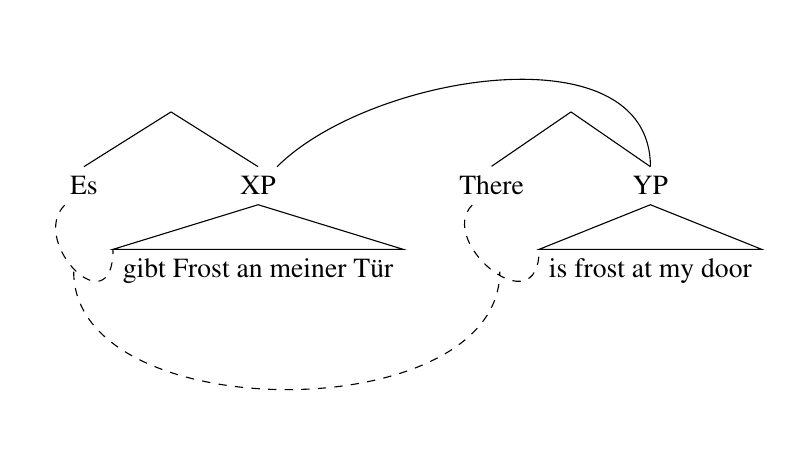
\begin{tikzpicture}
   \Tree [ [.\node(aDE){Es}; ]
    [.\node(pDE){XP};      
    \edge[roof]; \node(rDE){    gibt Frost an meiner Tür };  ] ] 
    \begin{scope}[shift={(2in,0in)}]
      \Tree [ [.\node(aEN){There};  ]
            [.\node(pEN){YP}; \edge[roof]; \node(rEN){ is frost at my door}; ] ]
          \end{scope}
          \draw[-] (pDE)..controls +(north east:2) and +(north:2) .. (pEN); 
          \draw[dashed,-] ($(rDE.west)-(0.5,0)$)..controls +(south:2) and +(south:2)..($(rEN.west)-(0.5,0)$); 
          \draw[dashed,-] (aEN)..controls +(south west:1) and +(south:1) .. (rEN.north west); 
          \draw[dashed,-] (aDE)..controls +(south west:1) and +(south:1) .. (rDE.north west); 
\end{tikzpicture}
   \caption{N-gram-samanstilling versus syntaktiske frasar}
    \label{fig:ikkjenode}
  \end{figure}

Men sett no at me ikkje har som formål å nytte frasesamanstillinga til
 reint N-grambasert omsetjing. Kva for \emph{lingvistiske} krav kan me
 stille til å kalle to frasar samanstilte? Me må i alle fall tillate
 ein del skilnad.  I alle større parallelltekster vil parallellstilte
 setningar ha visse syntaktiske og semantiske\footnote{Sidan eg går ut frå at data er setningssamanstilt, kjem eg
       ikkje inn på diskurs-/pragmatiske verknader, med mindre dette
       fører til forskjellar innanfor setningane (sjå t.d. del
       \ref{SEC:ordkrav} om lenkjer mellom koreferente substantiv og
       pronomen). } omsetjingsskifte,
 t.d. leksikalisering av syntaktiske konstruksjonar eller omvendt,
 endring av ordklasse, presisering/depresisering, endringar i
 leksikalske trekk (t.d. telleleg/utelleleg),
 osb. \citep[s.~56--62]{munday2001its}, slik at den einaste
 fullstendige, «perfekte» samanstillinga vil vere
 identitetsfunksjonen. Kor mykje mangel på samsvar me godtek blir då
 avgjort av formålet med samanstillinga.

Eitt av formåla med samanstillinga i denne oppgåva er å kunne oppdage
 korleis ulike språk realiserer semantiske roller syntaktisk; då
 spesielt i forhold til hypotesane gitt i \citet[s.~7]{xpar2008rcn},
 t.d. at «case marking might be useful to further determine a given
 argument's semantic role». Skal me finne det siste, må me altså kunne
 lenkje frasar med ulik kasusmarkering, men ha krav om lik tildeling
 av semantiske roller; samtidig skal me sjå at me ikkje kan ha krav om
 lik syntaktisk funksjon. I tillegg vil me sjølvsagt ikkje lenkje på
 tvers av konstituentgrenser, sidan det er fullstendige
 konstituentar\footnote{LFG tillèt som nemnt diskontinuerlege konstituentar, men dette
        er ikkje det same som ikkje-konstituentar av typen «es gibt» /
        «there is». } som fyller dei semantiske rollene.

Eit anna mogleg formål er å nytte desse frasesamanstillingane til
 maskinomsetjing. \citet{riezler2006gmt} nyttar ein frasesamanstilling
 (fått ved hjelp av N-gramtabellar) til å oppdage overføringsreglar
 for bruk i LFG-basert generering i maskinomsetjing. Dette er reglar
 som omsett fragment av ein f-struktur på kjeldespråket til
 f-strukturfragment på målspråket. (Eit krav på utforminga av moglege
 overføringsreglar hindrar at ein får reglar som lenkjar
 ikkje-konstituentar, eg kjem tilbake til dette nedanfor.) Ein
 liknande metode er \citet{graham2010dsl,graham2009fts}.
 Samanstillinga utvikla her burde au kunne nyttast til å finne slike
 overføringsreglar, men dette er ikkje noko eg har lagt vekt på.

Nedanfor gir eg eit forslag til krav for frasesamanstilling, med
 formåla nemnt her i tankane. Om alle krava er moglege å implementere,
 er eit separat problem.

\section{Frasesamanstilling i ein LFG-trebank}
\label{sec-3.3}


Samanstilte frasar bør ha nok semantisk likskap til å kunne opptre som
omsetjingar i liknande omgivnader
\citep[s.~74]{dyvik2009lmp}. \citet{thunes2003eal} gir nokre prinsipp
-- som er passande å ha som utgangspunkt -- for å fastslå det som kan
kallast \emph{omsetjingsmessig korrespondanse} (her for
ordsamanstilling). Dette er prinsipp som skal gjelde for eit litt
forskjellig formål, men som au «ligger nær opp til det vi intuitivt
mener er riktig» \citep[s.~2]{thunes2003eal}. Prinsippa blir nytta til
å lage ein gullstandard for ordsamanstilling\footnote{\cite[s.~2]{thunes2003eal}: «Våre prinsipper er satt
       opp for å tjene et bestemt formål, nemlig å samle inn data som
       metoden i Semantic Mirrors skal anvendes på», ein metode for å
       automatisk finne WordNet-liknande relasjonar frå
       parallelltekst. I denne metoden vil det vere naturleg med høge
       krav til presisjon, men kanskje lågare krav til dekning:
       speilmetoden skal finne leksikalske semantiske forhold som held
       på \emph{typenivå}, medan for trebanken er det viktigare korleis me
       kan annotere eit \emph{token} av t.d. eit verb i ein viss VP i ei
       gitt korpussetning. },
hovudsakleg for dei opne klassene, og er definert ved å vise til kva
for rolle eit argumentord speler, eller kva for rolletildeling eit
predikat eller modifiserande ord gir. Så for å t.d. samanstille to
verb må dei ha like mange semantiske argument (men argumenta treng
ikkje alle realiserast syntaktisk) og dei må \emph{tildele same roller};
medan argumenta må \emph{spele same rolle}, og både argument og adjunkt må
vere \emph{koreferente}. Lenkja ord må vere del av frasar som speler same
rolle i «det som er felles i interpretasjonene av [dei to setningane]»
\citep[s.~3]{thunes2003eal}.


Viss me tek utgangspunkt i det siste, vil det vere naturleg å i
tillegg lenkje desse frasane som speler same rolle i «det som er
felles i interpretasjonene».

Krava for ordsamanstillinga må au vere fylt for at desse frasane kan
samanstillast. Ei ordsamanstilling er altså naudsynt for ein
frasesamanstilling, og omvendt. Dette er berre problematisk om me
føreset at det eine er derivert av det andre; men dette har me ingen
\emph{a priori} grunn til å gjere. Krava eg her utviklar bør i staden
sjåast på som \emph{skrankar} på moglege samanstillingar i modellen (jamfør
\ref{SEC:omgrepsavklaring} om modellteoretiske grammatikkar), heller
enn derivasjonelle forhold. Samtidig er det som nemnt eit mål å finne
ut kor uavhengig me kan gjere oss av ordlenkjingsinformasjonen (dette
er au nyttig for implementasjonen), utan at det treng å gi krava ei
\emph{retning}.

Ei frasesamanstilling er ei skildring av forhold mellom \emph{fragment} av
setningar, dette er endå ein grunn til at det er naturleg å skildre
dei ønskelege forholda som skrankar på moglege samanstillingar. Me kan
setje skrankar på f-struktur-, konstituent- og ordsamanstilling
samtidig, utan å måtte ha krav om at den eine samanstillinga er
fullstendig (eller delvis) avleiia av den andre, før me veit om eit
slikt avleiingsforhold er empirisk fundert. Me kan i tillegg ha
ufullstendige samanstillingar i dei tilfella der det er ufullstendig
samsvar mellom setningane (der ei fullstendig samanstilling ville
brutt visse krav).

Sidan metoden er mynta på bruk i ein LFG-parsa trebank, og delvis vil
nytte denne annotasjonen som datagrunnlag, er det naturleg å nytte
same konsept som blir nytta i LFG\footnote{I tillegg finst andre positive biverknader av ein LFG-basert
       frasesamanstilling for bruk i denne samanhengen, som at ein kan
       studere kor parallelle dei parallelle grammatikkane i
       ParGram-prosjektet \citep{butt2002pgp} faktisk er, på ulike
       nivå (leksikon og argumentstruktur, c-struktur, f-struktur). } (f-struktur, c-struktur,
endosentrisitetsprinsipp, \xbar{}-tre, osb.)  au i desse krava til den
«beste» frasesamanstillinga; i den grad LFG gir ein generaliserbar
skildring av syntaks, bør desse krava vere generaliserbare til andre
teoriar, men ein del forhold som er avleidd av LFG-prinsipp må
sjølvsagt modifiserast om krava skal generaliserast til andre teoriar.

Utan skrankar i det heile vil alt kunne lenkjast til alt (noko som er
like unyttig som å ikkje lenkje noko); i del \ref{SEC:kandidatar} ser
eg på kva for typar element i dei lingvistiske analysane (ord,
grammatiske trekk, konstituentar, \ldots{}) det er fornuftig å tillate
lenkjer mellom. I avsnitta nedanfor spesifiserer eg kva som må til for
at me skal lenkje element av desse typane.

\section{Kva kan lenkjast?}
\label{sec-3.4}

\label{SEC:kandidatar}

Viss to uttrykk er samanstilt på setningsnivå (slik at me dimed kan gå
ut frå at dei er omsetjingar av kvarandre), og begge har ein
LFG-analyse, så har me iallfall tri ulike nivå kor me kan finne
ekvivalensforhold under setningsnivå:
\begin{enumerate}
\item mellom ord i setningane,
\item mellom f-strukturar,
\item mellom c-strukturnodar.
\end{enumerate}
På begge språk har me alle nivå -- det er ingen grunn til å lenkje på
tvers av nivå sidan forhold mellom desse nivåa er implisitt i
LFG-analysen.

Alle ord i setninga er \emph{kandidatar} for samanstilling med ord i
omsetjinga, men det kan godt hende at eit ord \emph{ikkje} har ei lenkje,
og me kan heller ikkje utelukke at det finst mange-til-mange-lenkjer
som ikkje kan «delast opp». Dette gjeld au nodane i c-strukturen.

Me utelukker lenkjing av ikkje-konstituentar som \emph{there is} på
c-strukturnivå sidan ei lenkje mellom to c-strukturnodar impliserer at
heile frasen under er lenkja. Det finst ingen c-strukturnodar som
dominerer berre \emph{there}, \emph{is} og ingen andre ord (heller ikkje \emph{es},
\emph{gibt}), så dette er ikkje lenkjekandidatar.  \emph{There is} og \emph{Es gibt}
i figur \ref{fig:ikkjenode} kan då ikkje samanstillast åleine, men
berre som del av ei ytre frasesamanstilling\footnote{Slike forhold kan me sjølvsagt finne igjen etter lenkjinga,
        men då vil me au kunne generalisere til andre ordformer. Eg
        kjem tilbake til dette i kapittel \ref{SEC:diskusjon}. }.

Når det gjeld f-strukturane er det ganske mange element me teoretisk
sett kunne ha lenkja, t.d. enkelttrekk som kasus eller dei uordna
mengdene med adjunkt, men det som er mest \emph{nyttig} og \emph{meiningsfullt}
er nok å berre lenkje der det er ei nær kopling til orda i
setninga. Sidan alle \PRED{}-element i ein f-struktur unikt står for
predikerande ord, kan me -- gitt to samanstilte setningar -- la
\emph{kandidatane for samanstilling på f-strukturnivå} inkludere alle
desse \PRED{}-elementa i f-strukturane til
setningane\footnote{I del \ref{SEC:fnord} kjem eg tilbake til spørsmålet om me vil
        inkludere visse f-strukturar utan \PRED{}-element i kandidatane
        for samanstilling. }. \PRED{}-element representerer semantiske bidrag som
oftast er påkrevde på begge språk i omsetjingar, medan andre
f-strukturtrekk gjerne er valfrie på det eine av språka; det er ikkje
alle språk som har t.d. obligatorisk kasusmarkering, og ein vil
kanskje nytte trebanken til å oppdage nettopp slik variasjon.
\PRED{}-elementa er i tillegg gjerne enklare å knyte direkte opp mot den
konkrete, observerte tekststrengen (eventuelt testast mot korpora,
eller talarintuisjonar), medan t.d. eit trekk som aspekt kanskje er
umogleg å skilje frå tempus i affikset (det vil vere vanskelegare å
teste om ei lenkje mellom aspekt-trekk er empirisk motivert utan å dra
inn ein heil del teori).

Samtidig er det au eit omsetjingsforhold mellom trekka i same
f-struktur som dei lenkja \PRED{}-elementa, og me ville kanskje ikkje ha
omsett dei to \PRED{}-elementa i andre f-strukturkontekstar. Difor bør me
au sjå på ei \PRED{}-lenkje som ei lenkje mellom \emph{f-strukturane til
desse \PRED{}-elementa}\footnote{Eventuelt kunne me ha definert lenkjingskandidatane på
       f-strukturnivå som alle \PRED{}-haldande f-strukturar, resultatet
       blir det same. }.  Med dette i tankane, kombinert med
c-struktur-f-strukturavbildinga $\phi$ (sjå del
\ref{SEC:omgrepsavklaring}), får me følgjande samanheng, illustrert i
figur \ref{fig:viss-PRED-så-f-og-c}:

\ex. \label{krav:f-links} Ei lenkje mellom to \PRED{}-element $p$ og $q$, kor
      $p$ er medlem av f-strukturen $f$, og $q$ er medlem av
      f-strukturen $g$, tilseier at:
\a. \label{krav:f-links-substr} me tolkar f-strukturane $f$ og $g$ som lenkja,
\b. \label{krav:f-links-words} orda i setningane som projiserer
     \PRED{}-elementa tek del i ei lenkje (kor andre
     ord kan vere involvert), og at
\c. \label{krav:f-links-domain} nodar innanfor $\phi^{-1}(f)$
     og $\phi^{-1}(g)$, dei funksjonelle domena til f-strukturane $f$
     og $g$, kan lenkjast

 \begin{figure}[htp]
    \centering
    \begin{tikzpicture}
    {\avmoptions{}
     \node(src){
        \begin{avm}
          $f$ \[pred  & `{\bf{}sove}<jeg>' \\
          tense & pret \\
          ... \]
        \end{avm}
      };
      \node[right of=src, node distance=5cm](trg){
        \begin{avm}
          $g$ \[pred   &  `{\bf{}sleep}<I>'\\
          tense  & pret  \\
          aspect & simple \\
          ... \]
        \end{avm}
      };
      }
      \draw[dashed,-] (src.west) .. controls +(-1,2) and +(-1,2) .. node[above,sloped]{$l_f$} (trg.west) ;
      \draw[-] ($(src.north)-(1,0.3)$) .. controls +(0,1.5) and +(0,1.5) .. node[above,sloped]{$l_p$} ($(trg.north)-(1,0.3)$) ;

      \begin{scope}[shift={(0,-3cm)}]
     \Tree  [.\node(VPs){VP}; [.\node(Vs){V}; \node(sov){sov};  ] ]
      \begin{scope}[shift={(5cm,0)}]
        \Tree  [.\node(VPt){VP}; [.\node(Vt){V}; \node(slept){slept};  ] ]
      \end{scope}
      \end{scope}
      \draw[-] (VPs)..controls +(north:1.5) and +(north:1.5) .. node[above,sloped]{$l_c$} (VPt) ;
      \draw[dashed,-] (sov)..controls +(north east:1.5) and +(north west:1.5) .. node[above,sloped]{$l_o$} (slept) ;
   \end{tikzpicture}
    
\fxnote{TODO: teikne inn f-domene}

    \caption{Ei \PRED{}-lenkje $l_p$ kan tolkast som ei f-strukturlenkje
    $l_f$, og impliserer ei c-strukturlenkje $l_c$ mellom toppnodane i
    dei funksjonelle domena. Orda som projiserer \PRED{}-elementa er med
    i ei lenkje $l_o$ (som kan inkludere fleire ord).}
   \label{fig:viss-PRED-så-f-og-c}
 \end{figure}

Punkt \ref{krav:f-links-substr} og \ref{krav:f-links-domain} over seier at viss
\PRED{}-elementa projisert av t.d. to verb i verbfrasar er lenkja, kan
VP-ane som heilskap lenkjast, i tilfellet i figur
\ref{fig:viss-PRED-så-f-og-c} kan iallfall dei øvste nodane i VP-ane
lenkjast, i tillegg til f-strukturane frå ytre \PRED{} til verba.  Det er
dette at heile VP-ane (kanskje inkludert objekt) er lenkja som gjer
det til ei fraselenkje og ikkje berre ei ordlenkje. Punkt
\ref{krav:f-links-substr} er forsvart over, medan punkt
\ref{krav:f-links-domain} kjem som ein konsekvens av at det er det
funksjonelle domenet som spesifiserer informasjonen i f-strukturane,
nodane her bør difor lenkjast berre viss f-strukturane er lenkja. Men
som punkt \ref{krav:f-links-domain} indikerer finst det au situasjonar der
nodar innanfor domena skal stå ulenkja.

Alle nodar i c-strukturen (alle syntaktiske \emph{frasar/konstituentar} i
setninga) som kan koplast til \PRED{}-haldande f-strukturar, vil vere
kandidatar for samanstilling på c-strukturnivå (dette inkluderer
diskontinuerlege konstituentar), men ikkje alle vil bli lenkja.  I del
\ref{SEC:subnode} ser eg på kva som må til for å lenkje nodar i det
funksjonelle domenet.  I tillegg finst det nodar over ord som ikkje
projiserer \PRED{}-element, desse kjem eg tilbake til i del
\ref{SEC:fnord}.

I følgje punkt \ref{krav:f-links-words} vil fraselenkja leie til at sjølve
verba i to lenkja VP-ar au er lenkja, som tilseier at \emph{ei \PRED{}-lenkje
impliserer ei ordlenkje}. I visse tilfelle er dette heilt
uproblematisk, t.d. viss \emph{I slept down by the river} skal lenkjast med
\emph{Eg sov nede med elva} vil me uansett lenkje \emph{slept} og \emph{sov}; dette
kan gjelde transitive verb au:

\ex. \a. The locusts have no king, just noise and hard language\\
     $\leftrightarrow$
     \b. Grashoppene har ingen konge, berre støy og krasse ord


\emph{have/har} tek del i VP-samanstillinga \emph{have no king.../har
ingen konge...}, her au skal det vere uproblematisk å lenkje
enkeltorda \emph{have} og \emph{har}.

Men som nemnd treng ikkje ordsamanstillinga vere ein-til-ein, det
punkt \ref{krav:f-links-words} seier er at desse orda iallfall er ein del
av ein samanstilling med kvarandre (i døme \Last altså
VP-samanstillinga). Kanskje er dette ei mange-til-mange-lenkje som
ikkje \emph{kan} reduserast til ein-til-ein-lenkjer; eller kanskje er
det som i \Last mogleg å skilje ut delsamanstillingar, som
\emph{have/har}. Eg kjem tilbake til dette
\fxnote[inline,nomargin]{TODO: når?} seinare.

Sidan \PRED{}-lenkjing impliserer ordlenkjing, må me sjekke om krava på
ordnivå (del \ref{SEC:ordkrav}) er oppfylte for å lenkje to
\PRED{}-element. \fxnote[inline,nomargin]{TODO: litt brå avslutning}

\section{Krav på ordnivå}
\label{sec-3.5}

\label{SEC:ordkrav}

Ord som skal lenkjast må i \cite{thunes2003eal} vere del av frasar som
speler same rolle i det som er felles i interpretasjonane, her kan me
omskrive det til at dei må vere del av \emph{frasar som er lenkja på c-strukturnivå}; forholda i \ref{krav:f-links} gir då koplinga til krav på
andre nivå (t.d. vil krav om tildeling av like mange roller vere
meir passande å spesifisere på f-strukturnivå).

Det er visse ting me ikkje kan spesifisere ut frå rein c- og
f-strukturinformasjon. Den norske setninga \emph{eg vil ete} kan fint
samanstillast med \emph{I want to eat}, med ei lenkje mellom \emph{ete} og
\emph{eat}. Men kva står i vegen for å lenkje \emph{ete} til hovudverbet i \emph{I want to drink}? Forskjellen på f-strukturnivå er berre at \PRED{}-verdien
er ulik (\textbf{eat} mot \textbf{drink}). Me må altså ha eit krav om at tydinga til
lenkja ord (og deira predikat) er «lik nok» til at me kan sjå på dei
som omsetjingar\footnote{Eigentleg burde slike setningar ikkje vere lenkja på
        setningsnivå ein gong, men som me skal sjå i del
        \ref{SEC:lik-argstr} treng me kravet om lik tyding 
        sjølv innanfor setninga. }. \citet[s.~74]{dyvik2009lmp} krev at orda
generelt, utan kontekst, må vere semantisk plausible omsetjingar,
dvs. at målordet er eit medlem av mengda av \emph{linguistically predictable translations} av kjeldeordet. Målordet har då
\emph{LPT-korrespondanse} med kjeldeordet.  Nedanfor reknar eg
LPT-kravet som eit krav på ordnivå, og eg føreset at LPT-informasjonen
er ein type bottom-up-informasjon, som viser om to ord generelt (i
ulike kontekstar) blir nytta som omsetjingar av kvarandre. Denne
informasjonen kan reint praktisk komme frå automatisk
ordsamanstilling, eller ei god tospråkleg ordbok, det bør ikkje spele
nokon rolle for resten av krava\footnote{Ein kan au tenkje seg at ei djup semantisk dekomponering av
        kvart ord sto som grunnlag for LPT-informasjon -- men då vil
        LPT-korrespondanse mellom to ord implisere at orda er
        synonyme, heller enn generelt plausible omsetjingar. }.

\fxnote{TODO: Er det mogleg å presisere LPT-kravet meir? Skal det
berre vere eit rangeringskrav??}
 
Ein type presisering/depresisering (del \ref{SEC:formaal}) me ofte ser
i omsetjingar er at eit pronomen på kjeldespråket blir nytta der
målspråket har eit koreferent substantiv, eller
omvendt. \citet{dyvik2009lmp} opnar for at desse au har
LPT-korrespondanse (som nemnt i \cite{thunes2003eal} må lenkja ord
uansett vere koreferente); om formålet vårt var maskinomsetjing heller
enn å byggje ein trebank for lingvistiske studie, ville det nok vore
betre å unngå slike lenkjer \citep[s.~53]{volk2008hjp}.

Men kva då med lenkjing av pronomen til verb bøygd for person og tal i
pro-drop-språk?

\ex. \a. iqePa                                  \hfill{} (georgisk) \\
     $\leftrightarrow$
     \b. han bjeffa

Viss setningane i døme \Last er lenkja, der iqePa har eit pro-argument
koreferent med \emph{han} som subjekt, bør dei to subjekta iallfall kunne
lenkjast på f-strukturnivå; dei har same referent og speler same rolle
i argumentstrukturen til verba (som me går ut frå er lenkja). På
ordnivå, derimot, kan me ikkje lenkje \emph{han} til \emph{iqePa} åleine -- her
må me ha ei mange-til-ein-lenkje mellom $\{ \rm han, bjeffa \}$ og $\{
\rm iqePa \}$. 
Generelt må me ha slike lenkjer der eitt ord projiserer fleire
\PRED{}-element\footnote{Me ville au fått ei mange-til-ein-lenkje om me tillot
        \emph{komplekse predikat} i analysane, t.d. slik
        \citet{butt1998merger} foreslår ved å la kombinasjonen av to
        ord endre argumentstrukturen til eitt \PRED{}-element. }.

\subsection{Ordklasse}
\label{sec-3.5.1}

Ulike språk leksikaliserer same konsept på ulike
måtar. \citet[s.~3]{cheung2002scg} nemnar vanskane med å ha eit krav
om lik ordklasse i utviklinga av ein kinesisk-engelsk termbank, kor
t.d. det engelske ordet \emph{fulfilment} meir naturleg blir omsett til eit
verb på kinesisk. På same måte vil eit georgisk verbalsubstantiv
(\emph{masdar}) gjerne bli omsett til eit verb i infinitiv på
norsk. Slike skifte mellom ordklasser er svært vanlege i
omsetjing\footnote{\citet[Catford~(1965),~i][s.~61]{munday2001its} gir ein gjennomgang av
       slike \emph{klasseskifte}, og andre typar omsetjingsskifte. }.

Me kan opne for ordklasseoverskridande lenkjer der det er samsvar på
andre nivå, me bør iallfall krevje ein likskap i argumentstruktur; så
om LPT-kravet og krava på c- og f-strukturnivå er fylt, bør det ikkje
vere noko i vegen for å lenkje ord (eventuelt mengder av ord) av ulik
ordklasse.


\section{Krav på f-strukturnivå}
\label{sec-3.6}

 
På f-strukturnivå har me direkte tilgang til informasjon om
argumentstrukturen til eit predikat, og mengda av adjunkt som
modifiserer predikatet. Når \citet[s.~3]{thunes2003eal} skriv at to
lenkja ord $a$ og $b$ må opptre i frasar som har «tilstrekkelig like
argumentstrukturer til at uttrykkene i \emph{a}s omgivelser står i de
samme semantiske relasjonene til hverandre og til \emph{a} som de
korresponderende uttrykkene i \emph{b}s omgivelser gjør til hverandre
og til \emph{b}» er det difor passande å prøve å gjere dette til eit
krav på f-strukturnivå.

Den enklaste lenkjingssituasjonen, f-strukturmessig, er der
rotpredikata kan lenkjast, og første argument av predikatet på
kjeldespråket kan lenkjast til første argument på målspråket, andre
argument til andre argument, osb., og lenkjinga kan fortsetje slik
rekursivt inn i f-strukturane\footnote{Når eg her skriv \emph{argument}, meiner eg eigentleg alle
        subkategoriserte ledd, både innanfor og utanfor sjølve
        argumentlista. I analysen av «eska opna seg» vil \emph{eske} stå
        innanfor argumentlista, medan refleksiven står utanfor:
        ${\avmoptions{center}\begin{avm}`{\bf{}opne}<eske>seg'\end{avm}}$.
        Begge er likevel subkategorisert for; begge er krevd av (den
        tydinga av) predikatet. }. I ein slik situasjon er det fullstendig
samsvar mellom kor mange argument det finst på kvar side, og
fullstendig samsvar i det tematiske rollehierarkiet (dvs. kva for
posisjon kvar rolle har i argumentstrukturen), i heile strukturen.

Som me skal sjå er det ikkje vanskeleg å komme over situasjonar der
dette ikkje held, og me blir nøydt til å tillate lenkjer mellom
argument og adjunkt, og lenkjer som går på tvers av følgja i
argumentstrukturane. I tillegg kan me ikkje klare oss utan
LPT-informasjon for å avgjere \emph{når} me har å gjere med slike meir
komplekse situasjonar. 
\subsection{Krav om lik argumentstruktur}
\label{sec-3.6.1}

\label{SEC:lik-argstr}

\citet{thunes2003eal} gir som nemnd eit krav om at \emph{predikat må ha tilsvarande semantiske argument} for å lenkjast.

Om det alltid er slik at to predikat har like mange argument, som kjem i
same rekkjefølgje i argumentstrukturen, vil det gjere den praktiske
oppgåva med å lenkje predikata, og argument med argument, mykje
enklare. Men kan me stille så sterke krav?

Sett at ei setning på språk 1 har ei \emph{at}-setning som adjunkt, medan
denne setninga på språk 2 er eit argument, og at desse setningane
ville vore lenkja om dei opptredde åleine. Om dei uttrykkjer same
proposisjon og \emph{speler same rolle i verbsituasjonen}, synest det
naturleg å lenkje desse.

Slike omsetjingsrelasjonar gir data for verbsituasjonen, på eit meir
generelt grunnlag enn det me kan få frå einspråklege analysar
åleine. Om me har gode semantiske grunnar for å kalle ein deltakar i
ein verbsituasjon eit argument på eitt språk, vil dei same grunnane
gjelde for omsetjingsmessig korresponderande verb på andre språk. Ein
kan då nytte unionen over alle argument til korresponderande verb til
å karakterisere kva ein meiner med \emph{deltakarane i verbsituasjonen}. Syntaktiske forhold i språket kan sjølvsagt gi
grunnar til å \emph{ikkje} kalle dette eit argument.

For å gjere dette konkret kan me sjå på følgjande setning frå
test-suiten til Xpar-prosjektet:

\exg. abramsi brouns       daenajleva sigaretze, rom cvimda \label{ex:vedde-gloss} \\
      Abrams.NOM Brown.DAT vedde.3SG sigarett.om, at  regne.3SG.IMP \\
     `Abrams veddet en sigarett med Brown på at det regnet' 

I følgje LFG-parsen til desse setningane har hovudpredikata svært ulik
argumentstruktur\footnote{Analysane er henta 18. mai, 2009, frå
        \href{http://decentius.aksis.uib.no/logon/xle.xml}{http://decentius.aksis.uib.no/logon/xle.xml}, som implementerer
        LFG-grammatikkane frå ParGram-prosjektet \citep{butt2002pgp}. }. Det norske \emph{vedde} har \underline{fire} argument, medan
\emph{da-najleveba} har \underline{to} (\emph{Abrams} og \emph{Browne}), kor at-setninga på
norsk og \emph{rom cvimda} uttrykkjer same proposisjon og speler same rolle
i verbsituasjonen. Den engelske LFG-parsen av den tilsvarande setninga
(mine omsetjingar) gir \underline{tri} argument, \emph{with} blir her adjunkt, medan
den tyske grammatikken, som au har \underline{tri} argument, gjer \emph{at}-setninga
til adjunkt. I \Next nedanfor har eg representert dei omsetjingsmessig
korresponderande frasane i f-strukturane med dei norske omsetjingane
for å illustrere dette:

{\avmoptions{}
\ex. \label{ex:vedde}
\a. Adams veddet en sigarett med Browne \hfill{} (norsk bokmål)\\ på at det regnet.\\
    $\\\begin{avm}\[pred & `{\bf{}vedde}<Abrams, sigarett, Browne, regne>' \\
                 adjunct & \{\}\]\end{avm}\\$
\b. abramsi brouns daenajleva sigaretze, rom cvimda. \hfill{} (georgisk)\\
    $\\\begin{avm}\[pred &  `{\bf{}da-najleveba}<Abrams, Browne, regne>'\\
    adjunct &  \{ \rm sigarett \}\]\end{avm}\\$ 
\c. Abrams hat mit Browne um eine Zigarette gewettet, \hfill{}(tysk)\\
    daß es regnet.\\
    $\\\begin{avm}\[pred & `{\bf{}wetten}<Abrams, regne>' \\
                  adjunct & \{ \rm Browne, sigarett \}\]\end{avm}\\$
\d. Abrams bet a cigarette with Brown that it was raining. \hfill{}(engelsk)\\
    $\\\begin{avm}\[pred & `{\bf{}bet}<Abrams, sigarett, regne>'\\
                  adjunct & \{ \rm Browne \}\]\end{avm}$

}

Om ein skal ha grammatikkane som datagrunnlag er det altså eit reellt
problem kva ein skal gjere med mangel på samsvar i
argumentstruktur. Om det alltid var fullstendig samsvar i
argumentstruktur, ville det vore trivielt å lenkje argument: viss to
korresponderande verb hadde tri argument, ville me lenkja det første
med det første, det andre med det andre og det tredje med det
tredje. Men om me har analysar som dei over, ser det ut til at me er
avhengig av LPT-kravet frå del \ref{SEC:ordkrav} for å avgjere kva for
adjunkt og argument som samsvarer. 

LPT-kravet blir forresten endå viktigare når det gjeld lenkjing av
adjunkt til adjunkt. Adjunkt plukker ut si eiga rolle (argument får
rolla tildelt frå verbet) og f-strukturane ordnar ikkje adjunkt etter
nokon rekkjefølgje, dei er representert som uordna mengder, medan
følgja mellom argument iallfall potensielt kan nyttast til å indikere
semantisk likskap.

Ein kan argumentere for at grammatikkane her \emph{burde} hatt like (eller
likare) analysar, dette ville letta lenkjingsarbeidet, men sidan stoda
no er slik, må krava ta høgd for lenkjer mellom argument og
adjunkt. Om seinare utgåver av grammatikkane gir likare analysar, vil
det iallfall ikkje gi verre lenkjingsresultat.

Og ei enkel korpusundersøking tyder på at det er relativt sjeldan at
ein får slike situasjonar som \Last illustrerer.  I
\citet{unhammer2009aaa} analyserte eg setningane frå den manuelt
frasesamanstilte trebanken SMULTRON \citep{samuelsson2006pap} med
LFG-grammatikkane for engelsk og tysk i ParGram-prosjektet
\citep{butt2002pgp}, for å undersøkje følgjande hypotese:
\begin{quote}
participants in a verbal situation are expressed as
arguments (rather than adjuncts) in the source language of a
translation if and only if they are expressed as arguments (rather
than adjuncts) in the target language.
\end{quote}

Mellom anna fann eg at 2 av 15 korresponderande verbtoken hadde
LFG-analysar kor argument korresponderte med adjunkt\footnote{25 om ein inkluderer analysar kor minst eitt av argumenta
        ikkje hadde korrekt analyse (t.d. eit \textsc{PRO} der
        grammatikken burde funne eit substantiv). }. Her
utgjorde altså dei grammatiske analysane (ein del av) data, og
undersøkinga seier nok meir om analysane enn om språklege forhold. På
et så tynt datagrunnlag kan me vel berre konstatere at me må kunne
handtere argument-adjunkt-lenkjer når me prøver å lenkje, men
argument-argument-lenkjer bør prioriterast viss alt anna er likt.

\subsection{Ulik følgje i argumentstruktur}
\label{sec-3.6.2}

I tillegg til at argument kan lenkjast til adjunkt, kan koreferente
argument ha ulik følgje i argumentstrukturen. Det er klart at me vil
lenkje objektet til \emph{gefallen} (eller bokmål: \emph{behage}) med subjektet
til \emph{like}, og omvendt.  Men rekkjefølgje i argumentstrukturane i
ParGram-prosjektet er ofte basert på syntaktisk funksjon heller enn
rolle, slik at eit verb som har tema som subjekt og opplevar som
objekt vil ha tema før opplevar i argumentstrukturen, medan ei
omsetjing av dette verbet kan ha opplevar før tema:

{\avmoptions{}
\ex. \a. der Tonfall gefällt mir nicht \\
     $\begin{avm}\[pred & `{\bf{}gefallen}<Tonfall, ich$_i$>' ... \]\end{avm}$
    $\\\\\leftrightarrow$\\
     \b. jeg liker ikke tonen \\
     $\begin{avm}\[pred & `{\bf{}like}<jeg$_i$, tonen>' ... \]\end{avm}$

}

Argumentstrukturane i \Last har omvendt intern følgje. Igjen må me ha
LPT-informasjon for å avgjere kva for lenkjing som er korrekt. Men i
visse tilfelle vil ikkje ein gong LPT-informasjon vere nok:

{\avmoptions{}
\ex. \a. sie$_j$ gefallen ihnen$_i$ \\
     $\begin{avm}\[pred & `{\bf{}gefallen}<de$_j$, de$_i$>' \]\end{avm}$
    $\\\\\leftrightarrow$\\
     \b. de$_i$ liker dem$_j$ \\
     $\begin{avm}\[pred & `{\bf{}like}<de$_i$, de$_j$>' \]\end{avm}$

}

Det finst ingen f-strukturinformasjon eller LPT-informasjon me kunne
nytta til å sikre den korrekte lenkjinga \emph{sie/dem} og \emph{ihnen/de}; og
viss me rangerer lik argumentstruktur over ulik, vil me her få feil
resultat. Det me \emph{kan} gjere (utanom å endre grammatikkane slik at
argumentstruktur korresponderer med eit universelt tematisk
rollehierarki) er å sjå på mange lenkjingar av same verbpar, og på den
måten oppdage moglege feil. For enkelttilfelle, derimot, vil krava i
denne oppgåva ikkje vere nok til å gi korrekt lenkjing.


\subsection{Krav om argumentlenkjer}
\label{sec-3.6.3}

Sjølv om me ikkje krev lik følgje i argumentlenkjer, og tillèt
argument-adjunkt-lenkjer, er det eit minstekrav for å lenkje to
\PRED{}-element at alle argumenta til det eine \PRED{}-elementet kan
korrespondere med argument eller adjunkt av det andre \PRED{}-elementet.
Dette følgjer av formålet med å finne ut korleis ulike språk
realiserer ulike semantiske roller syntaktisk; om eit verbargument
ikkje kan lenkjast til noko i omsetjinga (ikkje ein gong eit
pro-element), er det usannsynleg at verba uttrykker same situasjon, og
tildeler same roller. På same måte må sjølvsagt lenkja predikat ha
LPT-korrespondanse. \citet[s.~75]{dyvik2009lmp} gir følgjande krav på
f-strukturnivå\footnote{Med eit unntak for adposisjonsobjekt som eg kjem tilbake til i
        del \ref{SEC:adposisjonsobjekt}. }:

\ex. \label{krav:PRED} Krav for lenkjing av to \PRED{}-element $p$ og $q$:
\a. ordformene til $p$ og $q$ har LPT-korrespondanse
\b. alle argument av $p$ har LPT-korrespondanse med eit argument eller adjunkt av $q$
\c. alle argument av $q$ har LPT-korrespondanse med eit argument eller adjunkt av $p$
\d. LPT-korrespondansane kan lenkjast ein-til-ein
\e. ingen adjunkt til $p$ er lenkja til f-strukturar utanfor $q$, og omvendt

Det \Last[d] seier er at me ikkje lenkjer t.d. to instansar av «hest»
på det eine språket til éin instans av «horse» på det andre. Krav
\Last[e] kjem eg tilbake til nedanfor. 

Det går an å gjere \Last strengare, og krevje at argumenta -- i
tillegg til å ha LPT-korrespondanse -- sjølv er \PRED{}-lenkja. Dette har
eg ikkje gjort i implementasjonen min, men det er mogleg å ha det som
eit rangeringskriterium, noko eg kjem tilbake til i del
\ref{SEC:rangering}. Ved å \emph{ikkje} krevje at lenkjinga går heilt til
botn i f-strukturen blir det mogleg å seie at \emph{setningane} er
syntaktisk like, og at kanskje visse overordna frasar er syntaktisk
like, men visse \emph{delfrasar} kan likevel vere ulike og dimed ikkje vere
lenkja.

 Koordineringar har ikkje eit \PRED{}-trekk, men me handsamar dei som
 om dei hadde det. Alle dei koordinerte elementa er i ei \emph{mengd} i
 f-strukturen til koordineringa, og det er sjølvsagt ønskeleg å lenkje
 desse elementa om dei korresponderer:

 \ex. \label{krav:COORD} Ved lenkjing av f-strukturane til to
 koordineringar $p$ og $q$, sjå på dei som om elementa i mengdene var
 argument til eit \PRED{}-element, kor «argumentfølgja» er basert på
 setningsposisjon; $p$ og $q$ kan då lenkjast om dei oppfyller krav
 \ref{krav:PRED}.

 Argumentfølgje speler berre ei rolle i rangering, som eg kjem tilbake
 til i del \ref{SEC:rangering}.

Kva med f-strukturomgivnadene til $p$ og $q$, skal me krevje at dei er
like?  I \Last[e] har me eit krav om at adjunkt til $p$ ikkje er
lenkja til f-strukturar utanfor $q$, og omvendt. Men viss $a_p$ er eit
adjunkt til $p$, kan det lenkjast til ein \emph{dotternode} av argument
eller adjunkt til $q$? La $a_q$ vere eit argument eller adjunkt til
$q$, viss $a_q$ er eit argument må det ved \Last ha LPT-korrespondanse
med argument/adjunkt i $p$, men det treng ikkje vere lenkja -- viss
det er ulenkja gjeld ikkje krav \Last for $a_q$, så \Last hindrar
ikkje ei lenkje mellom $a_p$ og døtre av $a_q$. 

I tillegg vil ikkje \Last hindre at t.d. den yttarste f-strukturen i
kjeldespråket er lenkja til eit \XCOMP{}-argument på målspråket; men i
dette tilfellet bør kanskje ikkje \emph{setningane} vere lenkja i
utgangspunktet.

Sjølv om det er logisk mogleg å gjere slike lenkjingar, er det
vanskeleg å finne ikkje-vilkårlege avgrensingar for når ein skal kunne
lenkje f-strukturar som står i ulike omgivnader. I implementasjonen
min har eg difor følgt eit strengare krav enn \Last[e]:

\ex. \label{krav:PRED-omgivnad} \PRED{}-elementa $p$ og $q$ kan berre
     lenkjast om dei er yttarste f-strukturar i lenkja setningar, eller
     er argument/adjunkt til lenkja f-strukturar.

Dette er ei tentativ formulering. Til no har eg ikkje sett døme kor
\Last ikkje bør gjelde, men om det finst slike døme bør sjølvsagt
kravet modifiserast. Sidan LFG tillèt fragmentariske analysar kan det
vere \emph{fleire} yttarste f-strukturar, alle desse kan då potensielt
lenkjast med kvarandre, eller stå ulenkja (som om dei var adjunkt av
eit predikat som sto utanfor dei).

Krav \ref{krav:PRED} og \ref{krav:PRED-omgivnad} bør i enkle
situasjonar vere tilstrekkelege for lenkjing på f-strukturnivå, men
det finst au meir komplekse korrespondansar mellom \PRED{}-element. Desse
ser eg på del \ref{SEC:f-mange-mange}.


\subsection{Adposisjonsobjekt}
\label{sec-3.6.4}

\label{SEC:adposisjonsobjekt}

 I setningsparet i \ref{ex:vedde-gloss} har me eit objekt \emph{sigarett}
 som svarer til PP-en \emph{sigaretze} (\emph{sigareti} + \emph{ze}), som i \Next
 nedanfor:

{\avmoptions{}
\ex. \a. $\begin{avm}\[pred & `{\bf{}sigarett}' \]\end{avm}\\$
     $\\\leftrightarrow$\\
     \b.     $\begin{avm}\[pred & `{\bf{}ze}<\@{1}>' \\
                 obj & \@{1} \[pred & `{\bf{}sigareti}'\] \]\end{avm}$

}

 Medan \p{sigarett} er argument til \p{vedde}, står det ein adposisjon
 mellom \p{sigareti} og \p{da-najleveba}. I følgje krav
 \ref{krav:PRED} må me ha LPT-korrespondanse mellom \p{sigarett} og
 eit argument/adjunkt av \p{da-najleveba} for å lenkje \p{vedde} og
 \p{da-najleveba}, det har me ikkje -- det står ein adposisjon i vegen.

 Éi løysing ville vore å mange-mange-lenkje \p{sigarett} med
 \p{sigareti} og \p{ze} -- men dette gir ei misvisande lenkje, sidan
 \p{sigarett} ikkje bidreg med noko som tilsvarer den (syntaktiske)
 informasjonen som er gitt av \p{ze}. 

 Løysinga valt i \citet[s.~75,~fotnote~3]{dyvik2009lmp}, som eg
 følgjer i implementasjonen, er å berre hoppe over slike
 adposisjonar. Ved lenkjing av \p{vedde} og \p{da-najleveba} ser me
 då på f-strukturane i \Last som om dei var som i \Next nedanfor.

{\avmoptions{}
\ex. \a. $\begin{avm}\[pred & `{\bf{}sigarett}' \]\end{avm}\\$
     $\\\leftrightarrow$\\
     \b.     $\begin{avm}\[pred & `{\bf{}sigareti}' \]\end{avm}$

}

 Dette må ein altså ha i mente når ein følgjer krav \ref{krav:PRED}. I
 neste del diskuterer eg kva me kan gjere i dei situasjane der det
 ikkje er mogleg å berre hoppe over mellomliggande element.

\subsection{Kausativar og inkorporering}
\label{sec-3.6.5}

\label{SEC:f-mange-mange}
\fxnote{TODO: dette gjeld mange andre fenomen au, fryse ned, }

Til no har me føresett at eit \PRED{}-element anten er ulenkja, eller
er lenkja til eitt og berre eitt anna \PRED{}-element. Men i visse
tilfelle kan det vere ønskeleg å lenkje til fleire \PRED{}-element.

I ein norsk \emph{la}-konstruksjon, t.d. den me har i «å la noko fryse» (i
tydinga å forårsake at noko frys til) har me semantiske bidrag frå
både \emph{la} og hovudverbet \emph{fryse}, og begge har \PRED{}-element (sjølv om
bidraget frå \emph{la} nok er meir «grammatisk»). Men slike perifrastiske
konstruksjonar kan gjerne omsetjast til leksikaliserte kausativar som
berre har eitt \PRED{}-element, men likevel med tydinga «å la
fryse». Påfunnet i \Next illustrerer denne situasjonen:

{\avmoptions{}
\ex. \a. ho lar-fryse huset \\
     $\begin{avm}\[pred & `{\bf{}la-fryse}<ho, hus>' \]\end{avm}$
     $\\\\\leftrightarrow$\\
     \b. ho lar huset fryse \\
     $\begin{avm}\[pred & `{\bf{}la}<ho, hus, \@{1}>' \\
     xcomp & \@{1} \[pred & `{\bf{}fryse}<hus>'\]\]\end{avm}$

}

Her er altså den kausative tydinga leksikalisert, og verbet har berre
eitt \PRED{}-element (på same måte som det norske verbet \emph{kjøle} berre
har eitt \PRED{}-element, ikkje \emph{la} + \emph{bli kald}).\footnote{Det går sjølvsagt an å analysere sjølv leksikaliserte
        kausativar som om dei har fleire \PRED{}-element, men det bør i
        såfall skje på uavhengig grunnlag, ikkje for å gjere lenkjinga
        enklare. }

Den same situasjonen får me der eit argument eller adjunkt er
inkorporert i verbet på det eine språket, men uttrykt som eit separat
predikat på det andre språket, t.d. samisk \emph{fierpmástallat} som på
norsk blir \emph{å fiske med garn} -- to predikat på norsk tilsvarer eitt
på samisk.

I \Last har \emph{la-fryse} to argument, som ved krav \ref{krav:PRED} begge
må finne korresponderande argument eller adjunkt for å lenkje \emph{la-fryse}. 
Då går det ikkje an å lenkje \emph{la-fryse} til berre \emph{fryse},
som har eitt argument; me får eit \XCOMP{} til overs som manglar
lenkje. Me kan heller ikkje lenkje berre \emph{la} til \emph{la-fryse}, sidan
det då får ein \XCOMP{} til overs.

Det er mogleg å løyse dette formelt ved ei mange-mange-lenkje, kor ein
tenkjer seg \emph{la} og \emph{fryse} som samanføyd og at dei deler
argumentlister. Sidan begge verba tilfører viktig semantisk
informasjon, som er reflektert i den leksikaliserte kausativen, ville
det ikkje vore ønskeleg med ei ein-til-ein-lenkje sjølv om ein såg
vekk frå problemet med å lenkje argumenta.

Ved å ha ei ein-mange-lenkje, frå \emph{la-fryse} til både \emph{la} og \emph{fryse},
kan me oppfylle krav \ref{krav:PRED}. Då treng ikkje
\XCOMP{}-argumentet lenkjast til eit argument av \emph{la-fryse}, det er
allereie lenkja til \PRED{}-elementet; det som står igjen er unionen av
argumenta til \emph{la} og \emph{fryse}, desse må alle ha LPT-korrespondanse med
argument eller adjunkt av \emph{la-fryse}, og omvendt må alle argument av \emph{la-fryse} 
ha LPT-korrespondanse med argument eller adjunkt av \emph{la}
eller \emph{fryse} (utanom \XCOMP{}-argumentet til \emph{la}, som allereie har ei
lenkje). Ein kan tolke dette som om \emph{la} og \emph{fryse} var samanføyd til
eitt predikat som krevde to argument (her: \emph{ho} og \emph{huset}).

Den einaste formelle forskjellen mellom dette og
substantivinkorporering blir då at substantivet ikkje krev eigne
argument. Det er au mogleg å tenkje seg ein kausativ med eit
inkorporert objekt, omsett til \emph{la + hovudverb + objekt}, altså ei
lenkje frå eitt \PRED{} til tri \PRED{}. Igjen vil me då sjå på dei resterande
ulenkja argumenta på kvar side; kvar av desse må lenkjast med eit
unikt argument eller adjunkt.

Men det bør kanskje vere grenser for kor langt slik samanføying kan
gå, om ikkje anna fordi problemet fort blir komputasjonelt
vanskeleg. Å opne for ein-mange-lenkjer mellom \PRED{}-element (eller til
og med mange-mange-lenkjer) gir ei mykje større mengd moglege
løysingar på lenkjingsproblemet; i alle situasjonar der me krev
LPT-korrespondanse mellom eit argument $a_p$ av $p$ og eit adjunkt
$a_q$ av $q$ for å lenkje $p$ og $q$, vil me no au ha ei mogleg
løysing der $a_q$ er ulenkja, medan $a_p$ er samanføyd med $p$ og
difor ikkje treng LPT-korrespondanse med argument/adjunkt av $q$. Så
kan det au hende at $a_p$ sjølv kan samanføyast med eit av sine
argument/adjunkt. Skal me sjå etter slike løysingar samtidig som me
ser etter løysingar med ein-ein-lenkjer, vil me måtte leite gjennom
mange ufruktbare stigar. Ein måte å unngå dette på er å nedprioritere
samanføying, og berre prøve dette der det ikkje finst andre
alternativ.

Men det er ikkje berre av omsyn til implementasjonen ein bør
nedprioritere desse. Ei ein-mange-lenkje tyder på ein type
omsetjingsskifte, og det er ønskeleg å først sjå etter samanstillingar
som føreset syntaktisk likskap, før ein ser etter
omsetjingsskifte. Den viktigaste informasjonen me har å gå på er at
setningane er omsetjingar og difor har ein viss likskap -- Ockhams
barberkniv gir oss då grunn til å velje ei løysing som føreset lik
syntaks over ei løysing som føreset ulik syntaks. Viss det er mogleg å
opprette ei samanstilling på bakgrunn av lik syntaks, vil me
prioritere denne.

I implementasjonen blir difor alle ein-til-ein-lenkjer prøvd
først. Sidan kan ein prøve å føye saman eit ulenkja \PRED{}-element
$p$ med eit ulenkja \PRED{}-element $a_p$ kor $a_p$ er argument eller
adjunkt av $p$, og der $p$ og $a_p$ vil kunne lenkjast med eit ulenkja
\PRED{}-element $q$ ved føringane gitt over, og alle dei andre
lenkjingskrava er dekkja. Me får då ei modifisert utgåve av krav
\ref{krav:PRED}:

\ex. \label{krav:f-ein-mange} Krav for samanføyd lenkjing frå \PRED{}-elementa
$p$ og $a_p$, kor $a_p$ er eit argument eller adjunkt av $p$, til \PRED{}-elementet $q$:
\a. ordformene til $p$ og $a_p$ har saman LPT-korrespondanse med ordformen til $q$
\b. la $A$ vere unionen av argument til $p$ og argument til $a_p$,
    utanom $a_p$ sjølv;
    alle element av $A$ har LPT-korrespondanse med eit argument eller adjunkt av $q$
\c. la $D$ vere unionen av argument eller adjunkt til $p$ og argument
    eller adjunkt til $a_p$, utanom $a_p$ sjølv;
    alle argument av $q$ har LPT-korrespondanse med eit element av $D$
\d. LPT-korrespondansane er ein-til-ein
\e. ingen adjunkt til $p$ eller $a_p$ er lenkja til f-strukturar utanfor $q$, og ingen
    adjunkt til $q$ er lenkja til f-strukturar utanfor $p$

Det er trivielt å utvide dette kravet til å fungere for
mange-mange-lenkjer au; men til no har eg ikkje komme over situasjonar
som krev meir enn ein-mange/mange-ein-lenkjer, og implementasjonen min
held seg til desse for no.

\section{Krav på c-strukturnivå}
\label{sec-3.7}

\label{SEC:subnode}

Ein f-struktur er projisert av ei mengd c-strukturnodar, det vil seie
at det er desse nodane -- det funksjonelle domenet til f-strukturen --
som spesifiserer informasjonen som står i f-strukturen. Viss me har
grunnlag for å lenkje to f-strukturar, vil me au ha grunnlag for å
lenkje nodane som projiserte desse f-strukturane. Og omvendt vil det
aldri vere grunnlag for å ha ei c-strukturlenkje som står i konflikt
med f-strukturlenkjer, dvs. kor $\phi$ av kjeldenoden er lenkja til
noko anna enn $\phi$ av målnoden (då burde kjeldenoden vore lenkja til
dette andre). Det at to nodar er lenkja på c-strukturnivå må i det
minste implisere at informasjonen dei projiserer korresponderer. I
utgangspunktet bør krevje følgjande:

\ex.\label{krav:subnode-f-lenkja} to c-strukturnodar $n_s$ og $n_t$ kan
     berre lenkjast om $\phi(n_s)$ og $\phi(n_t)$ er lenkja på
     f-strukturnivå

Det enklaste ville vere å berre seie at alle nodane i dei to
funksjonelle domena er mange-mange-lenkja med kvarandre, men denne
lenkja vil ikkje gi oss meir informasjon enn at sjølve f-strukturane
er lenkja; ei lenkje på c-strukturnivå bør kunne gi meir nyansert
informasjon.

Det viktige forholdet på c-strukturnivå er \emph{dominans}; hovudgrunnen
til at me snakkar om c-struktur er at me vil skildre den hierarkiske
inndelinga av frasestrukturen i setninga, der ein node på høgare nivå
\emph{dominerer} mengder av nodar på lågare nivå. Ei lenkje mellom to
c-strukturnodar må altså implisere at det dominerte materialet
korresponderer.


\begin{figure}[htp]
\centering
  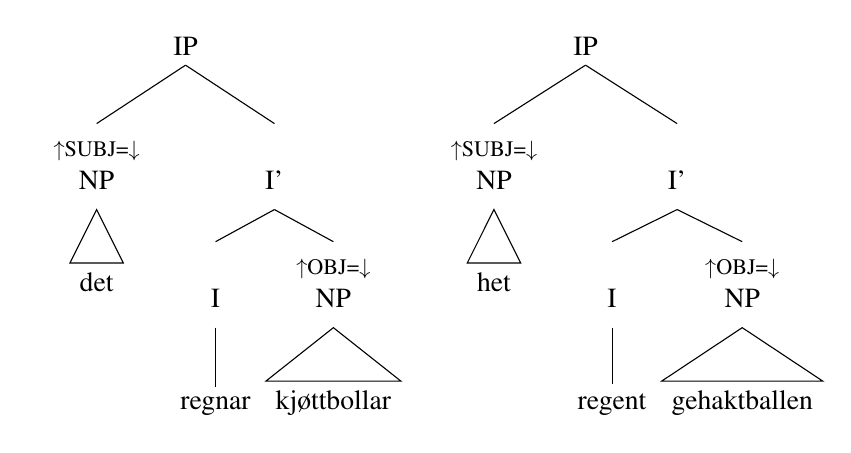
\begin{tikzpicture}
  \tikzset{level distance=1.5cm}
  \Tree  [.\node(IPs){IP};  [.\node(SUBJs){\proj{\ua SUBJ=\da}{NP}}; \edge[roof]; {det} ]
                            [.\node(I's){\proj{}{I'}};
                                    [.\node(Is){\proj{}{I}}; {regnar} ]
                                    [.\node(OBJs){\proj{\ua OBJ=\da}{NP}}; \edge[roof]; {kjøttbollar} ] ] ]
      \begin{scope}[shift={(2in,0in)}]
  \Tree  [.\node(IPt){IP};  [.\node(SUBJt){\proj{\ua SUBJ=\da}{NP}}; \edge[roof]; {het} ] 
                            [.\node(I't){\proj{}{I'}}; 
                                    [.\node(It){\proj{}{I}}; {regent} ]
                                    [.\node(OBJt){\proj{\ua OBJ=\da}{NP}}; \edge[roof]; {gehaktballen} ] ]   ]
\end{scope}
\end{tikzpicture}
   \caption{Enkel lenkjing av c-strukturnodar mellom norsk og
   nederlandsk; IP til IP, I' til I' og I til I.}
   \label{fig:enkel-c-lenkje}
  \fxnote{TODO: lenkjene!}
  \end{figure}

I figur \ref{fig:enkel-c-lenkje} er dei funksjonelle domena til \emph{regnar/regent} 
lenkja\footnote{I desse trea har eg annotert f-strukturforhold på visse nodar;
       der eg ikkje har teikna inn dette gjeld $\ua=\da$, altså at
       noden er i same funksjonelle domene som mornoden. Eg har i
       tillegg forenkla kategorinamna ein del frå dei som kjem direkte
       frå ParGram/Xpar-analysane, det bør ikkje ha noko å seie for
       framstillinga her. }, og det same med \emph{det/het} og \emph{kjøttbollar/gehaktballen}. 
Viss me føreset at subjekt-NP-ane er lenkja med kvarandre, og at
objekt-NP-ane er lenkja med kvarandre, på c-strukturnivå,
vil det vere ønskeleg å ein-ein-lenkje IP-nodane, I'-nodane og
I-nodane. Me skal sjå kvifor.

IP-nodane bør lenkjast sidan dei dominerer alt innanfor dei
lenkja funksjonelle domena; det finst ikkje ein gong nodar som står
utanfor det dei dominerer. Dei nodane som står nedanfor det funksjonelle
domenet til IP-ane er i tillegg lenkja med kvarandre. Det vil seie at
det ikkje finst informasjon på kjeldespråket som ikkje er uttrykt på
målspråket (eller omvendt) innanfor det IP-ane dominerer.

I'-nodane dominerer ikkje subjekta i figur
\ref{fig:enkel-c-lenkje}. Ei lenkjing av I'-nodane impliserer at det
som står under desse korresponderer, men au at nodane står i liknande
omgivnader. Det er lett å sjå føre seg eit døme der det ikkje ville
vore ønskeleg med ei lenkje mellom I'-nodane. I figur
\ref{fig:ikkje-c-lenkje} vil me t.d. ikkje lenkje desse nodane, på
norsk dominerer I' subjektet, som er lenkja til subjektet på
nederlandsk, men på nederlandsk står ikkje subjektet under I', og omvendt for
objektet. Ei lenkje mellom I'-nodane ville sagt at nodane dei
dominerte projiserte korresponderande informasjon, det gjer dei ikkje
i figur \ref{fig:ikkje-c-lenkje}. (I \ref{fig:enkel-c-lenkje}, derimot,
står dei lenkja objekta under I', medan dei lenkja subjekta er
utanfor.) Men merk at IP-nodane likevel kan lenkjast, dei dominerer
begge både subjekt og objekt, sjølv om dei kjem i ulik følgje under.
I-nodane dominerer berre verba, og kan au lenkjast.

\fxnote{nederlandsk kunne hatt inversion au!}

\begin{figure}[htp]
\centering
  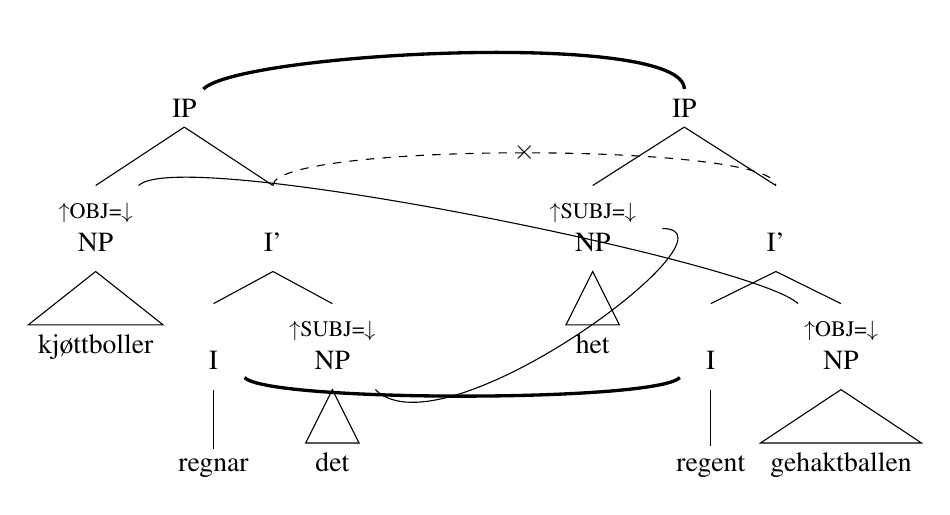
\begin{tikzpicture}
  \tikzset{level distance=1.5cm}
  \Tree  [.\node(IPs){IP};  [.\node(OBJs){\proj{\ua OBJ=\da}{NP}}; \edge[roof]; {kjøttboller} ]
                            [.\node(I's){\proj{}{I'}};
                                    [.\node(Is){\proj{}{I}}; {regnar} ]
                                    [.\node(SUBJs){\proj{\ua SUBJ=\da}{NP}}; \edge[roof]; {det} ]
                                     ] ]
      \begin{scope}[shift={(2.5in,0in)}]
  \Tree  [.\node(IPt){IP};  [.\node(SUBJt){\proj{\ua SUBJ=\da}{NP}}; \edge[roof]; {het} ] 
                            [.\node(I't){\proj{}{I'}}; 
                                    [.\node(It){\proj{}{I}}; {regent} ]
                                    [.\node(OBJt){\proj{\ua OBJ=\da}{NP}}; \edge[roof]; {gehaktballen} ] ]   ]
\end{scope}
\draw[-,very thick] (IPs)..controls +(north east:1) and +(north:1) .. (IPt) ;
\draw[dashed,-] (I's)..controls +(north:1.1) and +(north:1.1) .. node[midway,sloped]{$\times$} (I't) ;
\draw[-] (SUBJs)..controls +(south east:2) and +(east:2) ..  (SUBJt) ;
\draw[-] (OBJs)..controls +(north east:1.5) and +(north west:1.5) ..  (OBJt) ;
\draw[-,very thick] (Is)..controls +(south east:1) and +(south west:1) ..  (It) ;

\end{tikzpicture}
   \caption{C-strukturlenkjer kan ikkje gå på tvers av dominerte
   lenkjer (nynorsk og nederlandsk)}
   \label{fig:ikkje-c-lenkje}
  \end{figure}

Sjølv om subjektet sto ulenkja, t.d. ved lenkjing inn i eit
pro-drop-språk eller liknande, ville me fått same situasjon; I'-nodane
i figur \ref{fig:ikkje-c-lenkje-pro-drop} kan ikkje lenkjast sidan I'
på islandsk dominerer objektet, medan I' på norsk ikkje gjer dette, og
objekta er lenkja med kvarandre (her både på c- og f-strukturnivå). Ei
lenkje mellom desse I'-nodane ville sagt at dei dominerer
korresponderande materiale, men det gjer dei ikkje.

  \begin{figure}[htp]
  \centering
    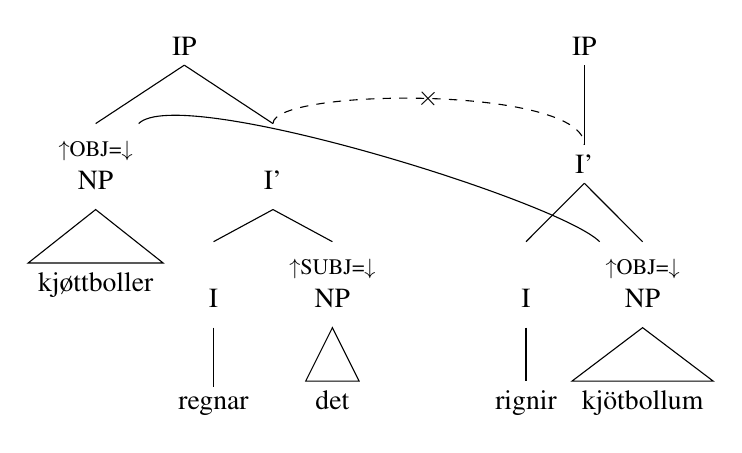
\begin{tikzpicture}
    \tikzset{level distance=1.5cm}
    \Tree  [.\node(IPs){IP};  [.\node(OBJs){\proj{\ua OBJ=\da}{NP}}; \edge[roof]; {kjøttboller} ]
                              [.\node(I's){\proj{}{I'}};
                                      [.\node(Is){\proj{}{I}}; {regnar} ]
                                      [.\node(SUBJs){\proj{\ua SUBJ=\da}{NP}}; \edge[roof]; {det} ]
                                       ] ]
        \begin{scope}[shift={(2in,0in)}]
    \Tree  [.\node(IPt){IP};  
                              [.\node(I't){I'}; 
                                      [.\node(It){\proj{}{I}}; {rignir} ]
                                      [.\node(OBJt){\proj{\ua OBJ=\da}{NP}}; \edge[roof]; {kjötbollum} ] ]   ]
  \end{scope}
\draw[dashed,-] (I's)..controls +(north:1) and +(north:1) .. node[midway,sloped]{$\times$} (I't) ;
\draw[-] (OBJs)..controls +(north east:1.5) and +(north west:1.5) ..  (OBJt) ;
  
  \end{tikzpicture}
     \caption{C-strukturlenkjer kan ikkje gå på tvers av dominerte
     lenkjer (nynorsk og islandsk)}
     \label{fig:ikkje-c-lenkje-pro-drop}
    \end{figure}


Når treet deler seg i to som i desse figurane, får me ei mogleg
oppdeling av kjeldene til f-strukturinformasjonen. Me vil ikkje lenkje
nodar som ikkje gir same tilskot til f-strukturen, på same måte som me
ikkje vil lenkje på tvers av f-strukturlenkjer.

I både figur \ref{fig:ikkje-c-lenkje} og figur
\ref{fig:ikkje-c-lenkje-pro-drop} er det slik at det I'-nodane dominerer gir
ulike tilskot til f-strukturen, dei kan difor ikkje lenkjast. Likevel
må me tillate litt slingringsmonn her, nodane skal ikkje trenge
projisere heilt like f-strukturar. Det som er relevant er det som blir
lenkja i f-strukturen.

Som desse døma viser må me nyansere prinsippet om å ikkje lenkje
c-strukturnodar på tvers av f-strukturlenkjer, til å ta innover
seg dominans: me vil ikkje lenkje c-strukturnodar viss \emph{det dei dominerer} kjem i konflikt med f-strukturlenkjer.


I visse tilfelle kan det hende at sjølv toppnodane i det funksjonelle
domenet ikkje bør lenkjast. I døma over dominerer toppnoden i det
funksjonelle domenet, IP, alt som står under $\phi(IP)$ i
f-strukturen.  I figur \ref{fig:ikkje-c-lenkje-toppnode}, derimot, er
objektet til \emph{regna} ikkje dominert av toppnoden i det funksjonelle
domenet til \emph{regna}, VP-en; men det er lenkja til objektet i
funksjonelle domenet til \emph{rained}. F-strukturane til dei to VP-ane er
lenkja, men toppnodane i dei funksjonelle domena kan ikkje lenkjast
sidan dei to toppnodane dominerer materiale som inneheld ulike lenkjer
på f-strukturnivå -- ei slik c-strukturlenkje ville stått i konflikt
med f-strukturlenkjene. Intuitivt synest det au feil med ei lenkje
mellom konstituentane \emph{det regner} og \emph{it rained meatballs}. Dei kan
iallfall ikkje reknast som omsetjingar av kvarandre åleine; i ein
større kontekst kan dei inngå i ein korrespondanse, men denne større
konteksten har me jo lenkja allereie ved IP-nodane.

  \begin{figure}[htp]
  \centering
    \begin{tikzpicture}
    \tikzset{level distance=1.5cm}
     \Tree  [.\node(IPs){IP};  [.\node(OBJs){\proj{\ua TOPIC=\da}{NP}}; \edge[roof]; {kjøttboller} ]
                               [.\node(I's){\proj{}{I'}};
                                       [.\node(Is){I}; {sa} ]
                                       [.\node(Ss){S};
                                               [.\node(SPKRs){\proj{\ua SUBJ=\da}{NP}}; {ho} ]
                                               [.\node(VPs){\proj{\ua COMP=\da}{VP}}; [.\node(SUBJs){\proj{\ua SUBJ=\da}{NP}}; \edge[roof]; {det} ]
                                                                                      [.\node(Vs){\proj{}{V}}; {regna} ] ] ] ] ]
         \begin{scope}[shift={(0in,-2.5in)}]
    \Tree  [.\node(IPs){IP};  [.\node(SPKRt){\proj{\ua SUBJ=\da}{NP}}; {she} ]
                               [.\node(I's){I'};
                                       [.\node(It){\proj{}{I}}; {said} ]
                                       [.\node(VPt){\proj{\ua COMP=\da}{VP}}; [.\node(SUBJt){\proj{\ua SUBJ=\da}{NP}}; \edge[roof]; {it} ]
                                                                              [.\node(V't){\proj{}{V'}}; [.\node(Vt){\proj{}{V}}; {rained} ]
                                                                                                [.\node(OBJt){\proj{\ua OBJ=\da}{NP}}; \edge[roof]; {meatballs} ]
 ] ] ] ]
  \end{scope}
  %\draw[-] (SPKRs)..controls +(south west:3) and +(west:3) ..  (SPKRt) ;
  \draw[dashed,-] (VPs)..controls +(north east:3) and +(east:4) ..  node[midway,sloped]{$\times$} (VPt) ;
  \draw[-] (OBJs)..controls +(west:4) and +(north east:3) ..  (OBJt) ;
  
  \end{tikzpicture}
     \caption{Sjølv toppnodane i eit funksjonelt domene kan stå
     ulenkja; her kan ikkje VP-nodane lenkjast sidan det norske
     \TOPIC{} er objektet til \emph{regna}, lenkja til objektet under
     VP på engelsk}
     \label{fig:ikkje-c-lenkje-toppnode}
    \end{figure}

I det minste bør me difor krevje følgjande av lenkjer på c-strukturnivå:
\ex.\label{krav:c-tentativt} Ein node $n_s$ kan lenkjast med ein node $n_t$ berre viss:
\a. $\phi(n_s)$ er lenkja på f-strukturnivå med $\phi(n_t)$, og
\b. det ikkje finst nodar under $n_s$ som er lenkja med nodar utanfor det funksjonelle domenet
    til $n_t$, og 
\c. det ikkje finst nodar under $n_t$ som er lenkja med nodar utanfor det funksjonelle domenet
    til $n_t$.

Men, kva om det finst nodar under $n_s$ som ikkje er lenkja på
c-strukturnivå (kanskje fordi det ikkje finst tilsvarande nodar på
målspråket, t.d. ved lenkjing inn i pro-drop-språk), men som har ei
lenkje på f-strukturnivå?  Her finst det fleire alternative løysingar,
som eg ser på nedanfor.

\subsection{Lenkja f-strukturar utan c-strukturnodar}
\label{sec-3.7.1}

\label{SEC:f-lenkje-utan-c-node}

I figur \ref{fig:gaiGo} kan iallfall IP-nodane lenkjast, dei dominerer
alle orda på begge setningane, og f-strukturane er lenkja. Men
NP-subjektet på den norske sida, er ikkje lenkja med noko i det
georgiske treet; dette subjektet er lenkja med eit pro-element på
f-strukturnivå. Den informasjonen (her reint syntaktisk) som ordet
\emph{det} tilfører IP, ligg under I' på georgisk. Ved I-nodane manglar
det norske treet i tillegg den informasjonen som \emph{seg} tilfører.

\begin{figure}[htp]
\centering
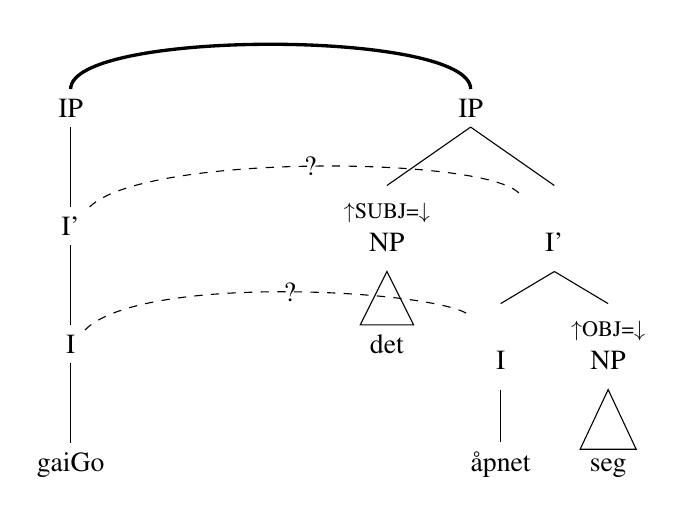
\begin{tikzpicture}
    \tikzset{level distance=1.5cm}
\Tree [.\node(IPk){IP}; 
  [.\node(Ibark){I'};  [. \node(Ik){I};  \node(gaiGo){gaiGo};  ]
  ] ]
     \begin{scope}[shift={(2in,0in)}]
\Tree [.\node(IPb){IP}; 
  [.\proj{\ua SUBJ=\da}{NP} \edge[roof]; {det} ] 
  [.\node(Ibarb){\proj{}{I'}};  [.\node(Ib){\proj{}{I}};   \node(åpnet){åpnet};  ]
       [.\proj{\ua OBJ=\da}{NP} \edge[roof]; {seg} ] ] ]
\end{scope}
 \draw[-,very thick] (IPk)..controls +(north:1) and +(north:1) .. (IPb) ;
  \draw[dashed,-] (Ibark)..controls +(north east:1.3) and +(north west:1.3) .. node[midway,sloped]{?}(Ibarb) ;
  \draw[dashed,-] (Ik)..controls +(north east:1.3) and +(north west:1) .. node[midway,sloped]{?}(Ib) ;
% \draw[-] (gaiGo)..controls +(south:1) and +(south:1) .. (åpnet) ;

\end{tikzpicture}
\caption{Skal ulenkja søsternodar hindre lenkjing? (Georgisk og bokmål)}
 \label{fig:gaiGo}
\end{figure}

Hadde det georgiske treet hatt spesifikator og komplement som kunne
lenkjast til spesifikator og komplement på norsk, ville det ha vore
uproblematisk å lenkje I' og I. Men om me berre har krav
\ref{krav:c-tentativt} å halde oss til, er det uspesifisert kva me
skal gjere i ein situasjon kor nodar lenkja på f-strukturnivå ikkje er
lenkja på c-strukturnivå.

Det finst (iallfall) to alternativ. 

Det eine alternativet er å seie seie at I- og I'-nodane ikkje skal
lenkjast, sidan \emph{det} og \emph{seg} er lenkja på f-strukturnivå (til
subjekt og objekt av gaiGo), då tolker me det slik at I' og IP
dominerer ulikt lenkja materiale. Det at det \emph{ikkje} finst ei lenkje
mellom I'-nodane, men mellom IP-nodane, vil då opplyse oss om at
I'-nodane dominerer ulike f-strukturlenkja informasjonstilskot på dei
ulike språka; likeins for I-nodane. Eg kjem tilbake til korleis ein
kan formalisere dette kravet i del \ref{SEC:c-strengare}.

 Det andre alternativet er å ikkje gjere forskjell på IP, I' og I når
 det gjeld c-strukturlenkjinga. Grunnen til å gjere dette er at
 \emph{gaiGo} både korresponderer med heile frasen \emph{det åpnet seg}, men au
 med berre \emph{åpnet seg}.  I figur \ref{fig:PanJara-gaiGo} ser me
 t.d. at I'-nodane kan lenkjast (utan å sjå på anna enn krav
 \ref{krav:c-tentativt}), det vil altså vere mogleg å lenkje I'-nodane
 i andre omgivnader. Det finst ein slags dobbeltheit mellom
 korrespondansen \emph{gaiGo-det åpnet seg} og korrespondansen \emph{gaiGo-åpnet  seg} og me kan uttrykkje dette ved å ikkje gjere forskjell på IP og
 I' i figur \ref{fig:gaiGo} (Dyvik 2010
 \citep{dyvik2010pc}).\fxnote[inline,nomargin]{har eg forstått dette
 rett? (korleis er dette ein korrespondanse på tokennivå?)}

\begin{figure}[htp]
\centering
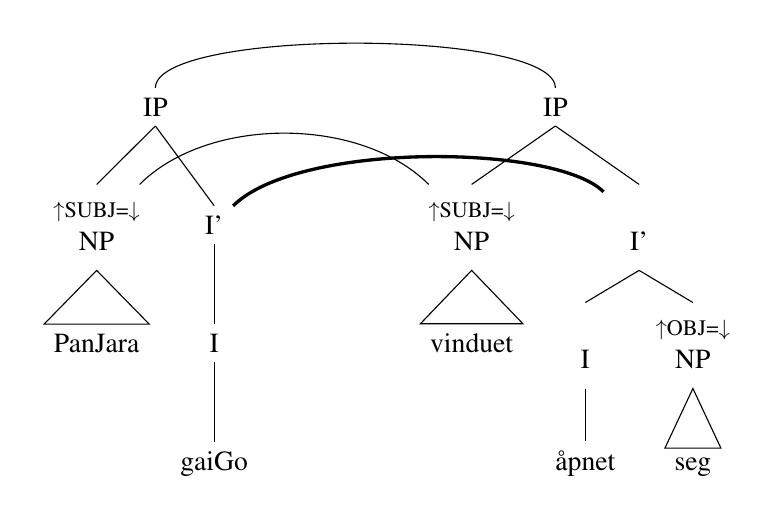
\begin{tikzpicture}
    \tikzset{level distance=1.5cm}
\Tree [.\node(IPs){IP}; 
  [.\node(NPs){\proj{\ua SUBJ=\da}{NP}}; \edge[roof]; {PanJara} ] 
  [.\node(I's){I'};  [.\node(Is){I};    \node(gaiGo){gaiGo};  ]
  ] ]
     \begin{scope}[shift={(2in,0in)}]
\Tree [.\node(IPt){IP}; 
  [.\node(NPt){\proj{\ua SUBJ=\da}{NP}}; \edge[roof]; {vinduet} ] 
  [.\node(I't){\proj{}{I'}};  [. \node(It){\proj{}{I}}; \node(åpnet){åpnet};  ]
       [.\proj{\ua OBJ=\da}{NP} \edge[roof]; {seg} ] ] ]
\end{scope}
 \draw[-] (IPs)..controls +(north:1) and +(north:1) .. (IPt) ;
  \draw[-,very thick] (I's)..controls +(north east:1.5) and +(north west:1.5) .. (I't) ;
%  \draw[dashed,-] (Is)..controls +(north east:1) and +(north west:1) .. node[midway,sloped]{$\times$}(It) ;
 \draw[-] (NPs)..controls +(north east:2) and +(north west:2) .. (NPt) ;

\end{tikzpicture}
\caption{Delvis mogleg lenkjing av underordna c-strukturnodar mellom georgisk og bokmål}
 \label{fig:PanJara-gaiGo}
\end{figure}


\citet[s.~77]{dyvik2009lmp} definerer i denne samanhengen
omgrepet \emph{lenkja leksikalske nodar}, $LL$, kor $LL(n)$ er mengda av
nodar dominert av $n$ som har ei ordlenkje. For å lenkje
c-strukturnodane $n_s$ og $n_t$, som er i lenkja funksjonelle domene,
må alle nodane i mengda $LL(n_s)$ vere lenkja til nodar i
$LL(n_t)$. Ulenkja nodar under $n_s$ og $n_t$ står ikkje i vegen for
lenkjing av $n_s$ og $n_t$, men dei to mengdene kan ikkje vere tomme.

Dette kravet gjer at ein ikkje treng krav \ref{krav:c-tentativt}, og
vil gi ei mange-mange-lenkje mellom alle nodane i dei to funksjonelle
domena til \emph{gaiGo-åpnet} i figur \ref{fig:gaiGo}. Viss me skriv ei
f-strukturlenkje som eit ordna par mellom \PRED{}-verdien på kjeldesida
(georgisk, med subskript $_s$) og \PRED{}-verdien på målsida (norsk, med
subskript $_t$) får me
$LL(IP_s)=LL(I'_s)=LL(I_s)=\{(\textbf{ga-Geba},\textbf{åpne})\}=LL(IP_t)=LL(I'_t)=LL(I_t)$
kor \emph{det} og \emph{seg} er ulenkja på både c-strukturnivå og ordnivå\footnote{\label{fn:LL-ordlenkje} Merk at orda \emph{det} og \emph{seg} måtte definerast som ulenkja for
        at denne definisjonen skulle fungere, noko som krev at ein nyanserer
        krav \ref{krav:f-links-words} litt. Viss me hadde definert
        \emph{det} og \emph{seg} som mange-ein-lenkja (med \emph{åpnet}) inn i
        \emph{gaiGo}, ville me fått same resultat som det krav
        \ref{krav:c-pro} i del \ref{SEC:c-strengare} gir.
        Viss georgisk er kjeldespråket
        ($n_s$, norsk: $n_t$) blir
        $LL(IP_s)=LL(I'_s)=LL(I_s)=\{(\text{gaiGo},\text{det}),(\text{gaiGo},\text{åpnet}),(\text{gaiGo},\text{seg})\}=LL(IP_t)$.
        Mengdene
        $LL(I'_t)=\{(\text{gaiGo},\text{åpnet}),(\text{gaiGo},\text{det})\}$
        og $LL(I_t)=\{(\text{gaiGo},\text{åpnet})\}$ på den norske
        sida har då ikkje korresponderande mengder på georgisk og blir
        ikkje lenkja. }.

\fxnote{TODO: diskutere litt meir forskjellane på desse alternativa}

\subsection{Eit strengare lenkjingskriterium}
\label{sec-3.7.2}

\label{SEC:c-strengare}

Sidan det er mogleg å ønskje seg å ikkje lenkje I'- og I-nodane i
\ref{fig:gaiGo}, gir eg her ein måte å formalisere dette på.

For å tillate lenkjene i figur \ref{fig:enkel-c-lenkje}, men ikkje dei
stipla lenkjene i figur \ref{fig:gaiGo}, ville det vore nok å krevje
at søsternodane var lenkja. I figur \ref{fig:enkel-c-lenkje} kan
I-nodane lenkjast fordi objekta er lenkja, I'-nodane fordi subjekta er
lenkja. I figur \ref{fig:gaiGo} kan dei norske I'- og I-nodane ikkje
lenkjast med noko fordi søstrene deira ikkje er lenkja.
Men dette blir for strengt. Det kan t.d. vere gode uavhengige grunnar
til å ha ein mellomliggande S-node før objektet på norsk, kor S er i
same funksjonelle domene som IP, medan det kanskje finst uavhengige grunnar
for å \emph{ikkje} gjere dette på andre språk. Figur
\ref{fig:enkel-c-lenkje-med-S} demonstrerer denne situasjonen. Her kan
ikkje S lenkjast til objektet sidan dei ikkje er i same funksjonelle
domene, men me vil jo likevel lenkje I-nodane; så eit krav om lenkja
søsternodar blir for strengt.

\begin{figure}[htp]
\centering
  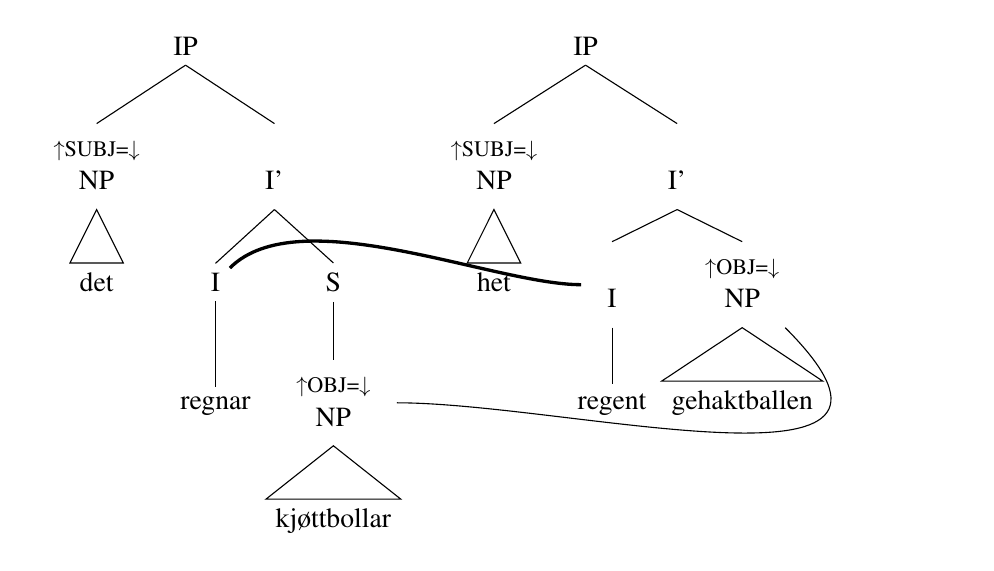
\begin{tikzpicture}
  \tikzset{level distance=1.5cm}
  \Tree  [.\node(IPs){IP};  [.\node(SUBJs){\proj{\ua SUBJ=\da}{NP}}; \edge[roof]; {det} ]
                            [.\node(I's){\proj{}{I'}};
                                    [.\node(Is){I}; {regnar} ]
                                    [.S [.\node(OBJs){\proj{\ua OBJ=\da}{NP}}; \edge[roof]; {kjøttbollar} ] ] ] ]
      \begin{scope}[shift={(2in,0in)}]
  \Tree  [.\node(IPt){IP};  [.\node(SUBJt){\proj{\ua SUBJ=\da}{NP}}; \edge[roof]; {het} ] 
                            [.\node(I't){\proj{}{I'}}; 
                                    [.\node(It){\proj{}{I}}; {regent} ]
                                    [.\node(OBJt){\proj{\ua OBJ=\da}{NP}}; \edge[roof]; {gehaktballen} ] ]   ]
\end{scope}
  \draw[-,very thick] (Is)..controls +(north east:1.5) and +(west:1.5) .. (It) ;
  \draw[-] (OBJs)..controls +(east:3) and +(south east:4) .. (OBJt) ;
\end{tikzpicture}
   \caption{I-nodane bør lenkjast sjølv om søsternodane ikkje er
   lenkja (norsk og nederlandsk)}
   \label{fig:enkel-c-lenkje-med-S}
  \end{figure}

Me treng altså eit litt meir nyansert krav. Som nemnt i fotnote
\ref{fn:LL-ordlenkje} går det an å få til dette ved ein kombinasjon av
konseptet om lenkja leksikalske nodar og å krevje at orda \emph{det},
 \emph{åpnet} og \emph{seg} i figur \ref{fig:gaiGo} er mange-mange-lenkja på
ordnivå til \emph{gaiGo}, sidan dei er lenkja til subjekt, predikat og
objekt av \emph{gaiGo} på f-strukturnivå. 

Men viss me vil unngå å referere til ordlenkjer, går det au an å
definere kravet i form av f-strukturlenkjer på preterminale
nodar\footnote{Då kan me au representere mange-til-mange-ordlenkjer som
        «udelelege», $(\{\text{gaiGo}\},\{\text{det,åpnet,seg}\})$
        blir den einaste ordlenkja i dømet over, sidan me ikkje må
        samanlikne ordlenkjene frå $IP_t$, $I'_t$ og $I_t$. }:

\ex. \label{krav:c-pro} For å lenkje c-strukturnodane $n_s$ og
     $n_t$:\\
     La $l_c(f)$ vere mengda som inneheld
     f-strukturlenkja til $f$, \emph{og} f-strukturlenkjene til alle
     argument $a$ av $f$ som ikkje har c-strukturnodar, dvs. kor
     $\phi^{-1}(a)=\emptyset$.
     La $L_c(n)$ vere mengda av $l_c(\phi(n'))$ for alle
     f-strukturlenkja preterminale $n'$ som er dominert av $n$.
     $n_s$ og $n_t$ kan lenkjast om $L_c(n_s)=L_c(n_t)$.

I figur \ref{fig:PanJara-gaiGo} har me då følgjande situasjon:\\
\\$L_c(IP_s)=\{(\textbf{PanJara},\textbf{vindu}),(\textbf{ga-Geba},\textbf{åpne}),(\textbf{pro},\textbf{seg})\}=L_c(IP_t)$
\\$L_c(I'_s)=\{(\textbf{ga-Geba},\textbf{åpne}),(\textbf{pro},\textbf{seg})\}=L_c(I'_t)$
\\$L_c(I_s)=\{(\textbf{ga-Geba},\textbf{åpne}),(\textbf{pro},\textbf{seg})\}
\neq \{(\textbf{ga-Geba},\textbf{åpne})\}=L_c(I_t)$\\

Dette vil seie at krav \ref{krav:c-pro} gir lenkjer mellom
IP-nodane og I'-nodane, men ikkje mellom I-nodane. I figur
\ref{fig:gaiGo} vil ikkje ein gong I'-nodane få ei lenkje, sidan den
norske I'-node dominerer 
$\{(\textbf{ga-Geba},\textbf{åpne}),(\textbf{pro},\textbf{seg})\}$
medan den georgiske I'-node dominerer
$\{(\textbf{pro},\textbf{det}),(\textbf{ga-Geba},\textbf{åpne}),(\textbf{pro},\textbf{seg})\}$,
det same som IP-nodane.

Merk at om me omdefinerer $l_c(f)$ til å ikkje innehalde
f-strukturlenkjer til argument av $a$, vil krav \ref{krav:c-pro} gi
same c-strukturlenkjer som kravet frå \cite{dyvik2009lmp}, men
definert i form av f-strukturlenkjer på preterminale nodar.
\subsection{Funksjonelle c-strukturnodar}
\label{sec-3.7.3}

\label{SEC:fnord}

Ikkje alle ord tilsvarer \PRED{}-element i f-strukturen, dette gjeld
 typisk funksjonsord (t.d. \emph{som}, \emph{at}). Ved endosentrisitetsprinsippa
 til \citet{bresnan2001lfs} er komplementet til funksjonelle
 kategoriar (C, I, P) ein funksjonell ko-kjerne, det er altså
 komplementet som gir \PRED{}-elementet i dette funksjonelle domenet.

Problemet med å nytte krava nemnt over i dette tilfellet er at nodar
 over funksjonsord er i det same funksjonelle domenet som
 komplementet, og nodane over funksjonsorda tilføyer ikkje ei ny
 \PRED{}-lenkje som kan dele opp treet slik me gjorde tidlegare. Så
 viss me vil lenkje desse nodane må me utvide prinsippa for å dele opp
 c-strukturtreet i buntar som dominerer same mengd med lenkjer.

Ord som ikkje projiserer \PRED{}-lenkjer kan likevel tenkjast å ha
 LPT-korrespondanse og bestå krava på ordnivå, men når me skal lenkje
 desse på c-strukturnivå må me då sjekke ordkrava direkte (me kan
 ikkje gå via nokon f-strukturlenkjing), så LPT-kravet gir oss eit
 utgangspunkt for lenkjing. Men dette avheng av korleis ein definerer
 LPT. Skal ein berre ta med semantisk tunge ord, eller bør
 funksjonsord au vere representert ved konseptet? Det kan
 argumenterast for at me ikkje bør la konseptet \emph{LPT-korrespondanse}
 dekkje funksjonsord, sidan det ofte (oftare enn med innhaldsord) er
 vanskeleg å seie på førehand kva ord desse kan omsetjast til; viss me
 trur me har avgrensa ei mengd med omsetjingar for eit funksjonsord,
 men så finn det omsett til eit nytt funksjonsord -- kor dei semantisk
 tunge komplementa bør lenkjast, og konteksten er lik -- så bør nok
 det heller vere evidens for at desse to funksjonsorda au er moglege
 omsetjingar \citep{dyvik2010pc}.  I såfall har me ikkje fleire
 lenkjingskrav for funksjonelle nodar, og ser på dei preterminale
 funksjonelle nodane som om dei ikkje dominerte noko; eller: $L_c$
 (evt. $LL$) av desse nodane er tomt.

Men, det kan sjølvsagt hende at ein ønskjer å setje eit LPT-krav på
 ord som ikkje projiserer noko \PRED{}-element, der ein er svært
 sikker på dei moglege omsetjingane (t.d. der ei viss ikkje-omsetjing
 av eit funksjonsord kan føre til logisk motsett tyding). Sidan det er
 mogleg å ønskje seg slike krav, gir eg her eit forslag til korleis
 det kan formaliserast.

Viss me har to funksjonelle konstituentar kor komplementa kan lenkjast
 på f-strukturnivå, men funksjonsorda ikkje kan sjåast på som moglege
 omsetjingar (t.d. \emph{fordi} og \emph{whether}), kan det hende ein ikkje ein
 gong vil lenkje komplementa. Ein kan sjå på dette som at
 funksjonsorda gjer at komplementa speler ulike roller i
 omgivnadene\footnote{Skal ein lenkje ordet \emph{som} (utan \PRED{}) med ordet \emph{which} (med
        \PRED{})? Viss krava elles er oppfylt, kan det kanskje vere
        informativt med ein type «defekt» lenkje, sjølv om berre det
        eine ordet blir rekna for å vere eit innhaldsord. Frasane til
        deira funksjonelle domene vil uansett kunne lenkjast viss dei andre
        krava er oppfylte. }. Samtidig vil me nok ikkje at eit manglande
 funksjonsord på det eine språket skal hindre lenkjing av komplementa,
 sidan det kan hende at funksjonsordet ikkje er krevd på det språket
 (eventuelt kjem dette fram som korrespondansar i f-strukturtrekk, eg
 har ikkje teke høgd for korrespondansar mellom andre
 f-strukturelement enn \PRED{} i denne oppgåva).

Me kan krevje at komplementa er lenkja for å sikre at me ikkje lenkjer
 nodar som står i ulike konstekstar (me vil ikkje lenkje \emph{at} i «han
 såg at det gjekk bra» med \emph{that} i «he saw that she drew a picture»),
 jamfør kravet om lenkja argument for lenkja predikat i del
 \ref{SEC:lik-argstr}.

Desse ønskene kan me formalisere slik:

\ex. \label{fnordkrav} Krav for lenkjing av funksjonelle kategoriar i
    c-strukturen, viss funksjonsord er dekkja av LPT-krav:
\a. Gitt ei mogleg lenkjing av FP og GP, kor F og G er funksjonelle
    kategoriar der komplementa elles kan lenkjast,
    tolk LPT-korrespondansen mellom orda under F' og G' som eit
    medlem av lenkjemengda $L_c$ (evt. $LL$), kor denne må vere lik
    for at FP og GP skal kunne lenkjast. Då kan me au lenkje F' og G'.
\b. Gitt ei mogleg lenkjing av FP og XP, der F er ein funksjonell
    kategori, medan X er ein ikkje-funksjonell kategori, ignorerer me
    den funksjonelle kategorien i c-strukturlenkjinga. Sidan det ikkje
    er nokon forskjell i $L_c$ (evt. $LL$) mellom FP og F', er F' medlem
    av nodemengden som blir lenkja til XP.

Om \Last[a] er oppfylt, kan me få samanstillinga vist i figur
 \ref{fig:fnord}. Her vil dei funksjonelle domena til CP og CP kvar
 kunne delast opp i to delar, kor den funksjonelle delen har
 LPT-korrespondanse medan komplementa er lenkja på
 f-strukturnivå. Lenkjemengdene under CP-nodane er like, og dei under
 C-nodane er like. Merk at me får same samanstilling om me ikkje har
 noko LPT-krav på ord utan \PRED{}-element -- utanom at dei
 preterminale C-nodane då står ulenkja.

(Alle nodane under S vist i dei to trea er i same funksjonelle domene,
 så om dei funksjonelle domena er lenkja, vil krav
 \ref{krav:subnode-f-lenkja} vere oppfylt kva gjeld CP-komplementa --
 lenkjinga går ikkje ut over dei funksjonelle domena, medan krav
 \ref{krav:c-pro} er dekkja for S-nodane med unntaket over.)

  \begin{figure}[htp]
   \centering
  
  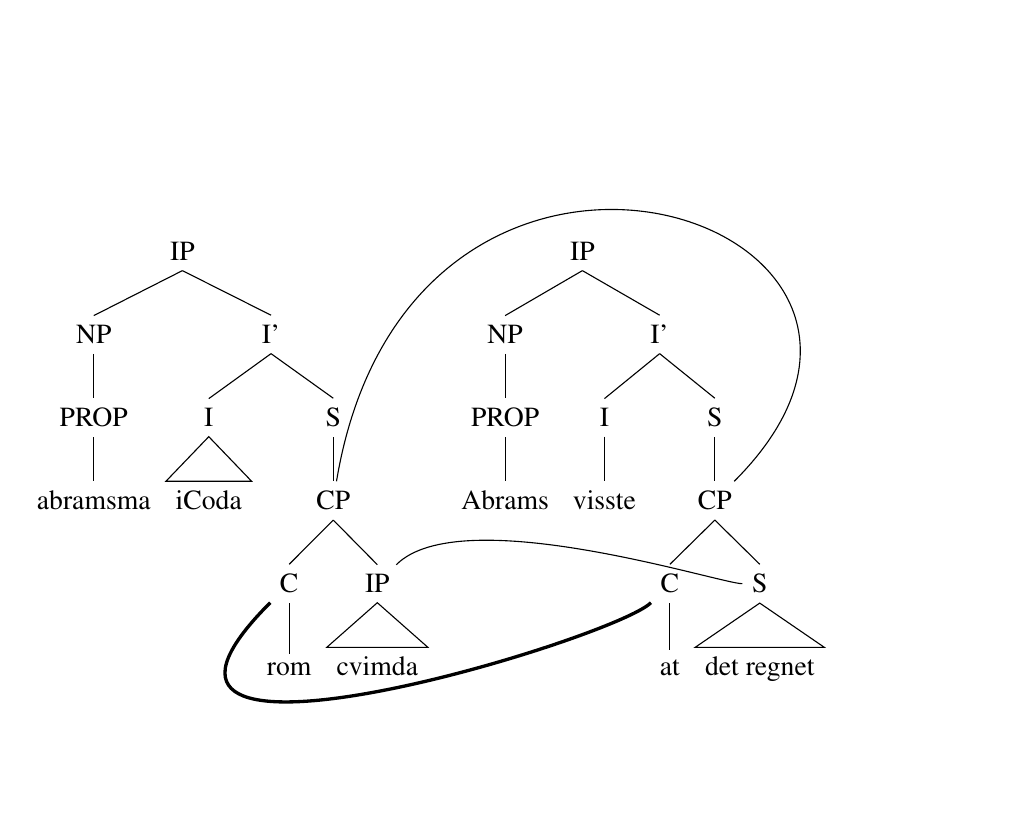
\begin{tikzpicture}
  \Tree
  [.IP
    [.NP [.PROP abramsma ] ] 
    [.I' [.I \edge[roof]; {iCoda} ]
             [.S [.\node(CPs){CP};
                  [.\node(Cs){C};  rom ]
                  [.\node(IPs){IP}; \edge[roof]; {cvimda} ]]]]]
      \begin{scope}[shift={(2in,0in)}]
  \Tree
  [.IP
    [.NP [.PROP Abrams ] ]
     [.I' [.I visste ]
              [.S  [.\node(CPt){CP};
                   [.\node(Ct){C};  at ] 
                   [.\node(St){S}; \edge[roof]; {det regnet} ]]]] ]
  \end{scope}                      
  \draw[-] (CPs)..controls +(1,6) and +(north east:5) .. (CPt) ;
  \draw[-] (IPs)..controls +(north east:1.5) and +(west:0.5) .. (St) ;
  \draw[-,very thick] (Cs)..controls +(south west:4) and +(south west:1) .. (Ct) ;
  \end{tikzpicture}
  \caption{Mogleg samanstilling av funksjonelle c-strukturnodar mellom georgisk og norsk (bokmål)}
   \label{fig:fnord}
  \end{figure}

Der det eine språket har eit funksjonsord og det andre språket ikkje
 krever det, bryr me oss ikkje om funksjonsordet. For å sjekke noko
 slikt må me som nemnt sjå på andre trekk enn \PRED{} i f-strukturane,
 noko som blir utanfor denne oppgåva; men om me hadde sjekka slike
 f-strukturkorrespondansar kunne me unngått kravet om
 LPT-korrespondanse og i staden nytta informasjon frå f-strukturane
 til lenkjing av funksjonelle kategoriar. Utan å ha slike mekanismar
 på plass blir f-strukturlenkjinga avhengig av c-strukturforhold, og i
 implementasjonen min har eg difor valt å ikkje lenkje ord som ikkje
 projiserer \PRED{}-element.

\section{Rangering}
\label{sec-3.8}

   \label{SEC:rangering}

Gitt ei viss f-struktursamanstilling, vil det berre vere éin mogleg
måte å lenkje på c-strukturnivå. Men slik f-strukturkrava er stilt,
kan me få mange ulike moglege samanstillingar på
f-strukturnivå. Ideelt sett burde krava vere nyanserte nok til å
plukke ut berre dei samanstillingane som er ønskelege, men som vist
over er dette ikkje alltid like lett, spesielt om me ikkje har
fullstendig informasjon om LPT-korrespondansar.

Difor er det nyttig å ha nokre kriterium, eller i det minste
heuristikkar, for å rangere ulike f-struktursamanstillingar. Det er
sjølvsagt svært mange måtar ein kan rangere to strukturar på; kriteria
nedanfor er tenkt å gi dei samanstillingane som føreset at
argumentstrukturane er så like som mogleg. Implementasjonen av
kriteria kjem i del \ref{SEC:impl-f-rangering}.

Merk at om me har «fullstendig» LPT-informasjon (t.d. ei perfekt
omsetjingsordbok), treng me aldri rangere. Desse kriteria er difor
kanskje mindre teoretisk interessante, sidan dei alltid kan
overstyrast ved å gi systemet meir kunnskap. Men det kan au vere
interessant å teste kor godt ulike rangeringskriterium fungerer der me
ikkje har LPT-informasjon i det heile -- då vil dei i prinsippet
fungere som «mjuke» skrankar på f-struktursamanstillinga.

Nedanfor følgjer dei kriteria eg har basert implementasjonen på. Som
nemnt er det berre ein av mange moglege måtar å gjere det på, men
kriteria tek innover seg dei trekka som er relevante for
argumentstrukturen: argumentfølgje og rekursiv f-strukturlenkjing.

\subsection{Rangering ved følgje}
\label{sec-3.8.1}

I \citet[s.~75--76]{dyvik2009lmp} blir det formulert eit
spesialtilfelle av krava for lenkjing på f-strukturnivå, der det er
like mange argument på kvart predikat, og førsteargument er lenkja til
førsteargument, andre til andre, osb. I slike situasjonar er ingen
adjunkt lenkja til argument; og om argumentstrukturane i analysane
reflekterer det semantiske rollehierarkiet, vil me aldri lenkje
t.d. agens til patiens og patiens til agens. Der grammatikkane er
skrivne etter parallelle prinsipp, bør ei slik samanstilling -- om alt
anna er likt -- gi den ønskelege lenkjinga.

Difor har me dette som eit rangeringskriterium. For å nyansere det
litt, kan me sjå på kor mange av lenkjene frå argumenta til eit
predikat som ikkje er argument-adjunkt-lenkjer, og der dei ikkje har
ulik posisjon i argumentstrukturen. Meir formelt:

\ex. \label{krav:arg-order-rate} La $m$ vere mengda av ein-til-ein
     LPT-korresponderande argument/adjunkt av to lenkja f-strukturar
     $F_s$ og $F_t$. La $n$ vere dei elementa av $m$ som anten begge
     er adjunkt, eller begge er argument og har same posisjon i
     argumentstrukturane sine. \emph{Følgjeskåren} til $F_s$, $F_t$ er då
     $\frac{n}{m}$.

I spesialtilfellet nemnt over, vil skåren altså vere 1. Når det står
«ein-til-ein LPT-korresponderande» over, er det for å plukke ut ein
viss måte å samanstille argumenta og adjunkta til $F_s$ og $F_t$ --
men utan krav om at desse skal vere rekursivt lenkja. Kriteriet
nedanfor rangerer rekursive lenkjer høgare enn enkle
LPT-korrespondansar.

\subsection{Rangering ved djupn}
\label{sec-3.8.2}

Krav \ref{krav:PRED} krev ein-til-ein LPT-korrespondanse mellom
argument/adjunkt av kjelde- og målpredikatet, men stiller ikkje krav
om at dei LPT-korresponderande elementa sjølv må vere lenkja på
f-strukturnivå. Så viss «She tried to ride a bike» er lenkja med «Ho
prøvde å sykle», kan me lenkje \emph{try} med \emph{prøve} sjølv om \emph{ride} og
\emph{sykle} ikkje kan lenkjast -- \emph{bike} er eit påkravd argument\footnote{Merk: utan meir informasjon her vil krava i tillegg opne for
        ei mange-mange-lenkje mellom \emph{ride} + \emph{bike} og \emph{sykle}; for
        skuld argumentet ser me berre på ein-til-ein-lenkjer her. }. I
situasjonar der me har eit val mellom berre LPT-korrespondanse, og
full rekursiv lenkjing, vil ei rekursiv lenkje skildre meir
strukturell likskap enn berre LPT-korrespondansen.

Difor har me dette som eit rangeringskriterium. Me kan formalisere det
slik:

\ex. \label{krav:sub-f-rate} La $m$ vere mengda av ein-til-ein
     LPT-korresponderande argument/adjunkt av to lenkja f-strukturar
     $F_s$ og $F_t$. La $n$ vere dei elementa av $m$ som anten ikkje
     har argument sjølve, eller som er lenkja på
     f-strukturnivå. \emph{Djupnskåren} til $F_s$, $F_t$ er då
     $\frac{n}{m}$.

Der alle LPT-korresponderande argument/adjunkt av $F_s$ og $F_t$ au er
lenkja, vil djupnskåren vere 1.

\subsection{Rangering for heile samanstillinga}
\label{sec-3.8.3}

Kriteria over gir to skårer for eit visst par av \PRED{}-element. Utan å
ha testa desse kriteria empirisk er det naturleg å vekte dei likt;
altså bør skåren for eitt par av \PRED{}-element innehalde produktet av
desse skårane.

Men argumenta og adjunkta av desse to elementa kan sjølv ha ulike
moglege delsamanstillingar, som kan gi ulike skårer. La $a_s$ og
$a_t$, argument eller adjunkt av $F_s$ og $F_t$, vere lenkja i ei
mogleg samanstilling av $F_s$ og $F_t$. Innanfor $a_s$, $a_t$ finn me
kanskje ulike moglege samanstillingar, her vel me den som gir best
skåre. Men det kan hende at det finst ei alternativ måte å lenkje på,
kor $F_s$ er lenkja til $G_t$, $a_s$ til $d_t$ (argument/adjunkt av
$G_t$), og $a_s$, $b_t$ har høgare skåre enn $a_s$, $a_t$. Viss alt
anna er likt, bør me då heller velje $F_s$, $G_t$ enn $F_s$, $F_t$.

Den endelege skåren for $F_s$, $F_t$ er då produktet av følgjeskåren,
djupnskåren og den vekta summen av dei endelege skårane for lenkja
argument/adjunkt av $F_s$ og $F_t$. Denne summen er vekta på lengden
av lista med lenkja argument/adjunkt, for å ikkje gi unaturleg høg
skåre til f-strukturar med mange argument/adjunkt; men viss me til
slutt har mange greiner med same skåre, vel me den lengste sidan den
då har flest lenkja adjunkt\footnote{Dette er ganske \emph{ad hoc} skåringsfunksjon, og det er ikkje
        sikkert at alle kriteria bør ha lik vekting.  Sidan det ikkje
        er meininga å nytte denne skåringa i maskinlæring har eg ikkje
        undersøkt om dette kan gjerast til ein stringent
        sannsynsmodell (der summen av skårar for alle moglege
        samanstillingar aldri går over 1); men det bør vere mogleg å
        gjere noko slikt ut av det. }.



\section{Oppsummering}
\label{sec-3.9}

Krava formulert i denne delen definerer kva for lenkjer som er
ønskelege mellom konstituentar og mellom f-strukturar, når formålet er
å annotere ein parallell trebank for lingvistiske studium. Det finst
visse tilfelle der krava \emph{ikkje} kan avgjere kva som er den ideelle
lenkja utan meir informasjon enn det dei grammatiske analysane gir; eg
diskuterer slike døme i kapittel \ref{SEC:diskusjon}, i tillegg til
døme som er problematiske for krava sjølv der me har fullstendig
informasjon, og der meir arbeid trengst. Kapittelet som kjem no gir
detaljane for programmet \texttt{lfgalign}, som implementerer krava frå dette
kapittelet sånn at det er lettare å teste kor dei slår feil.


\chapter{Implementasjonen av \texttt{lfgalign}}
\label{sec-4}

\label{SEC:implementasjon}

  % \begin{quotation}
  % Scientists reproduce results; engineers build impressive and enduring
  % artifacts; and theologians muse about what they believe but can't see
  % or prove.
  % \begin{minipage}{0.77\textwidth}
  % \begin{flushright}
  % \citep[s.~466]{pedersen2008enm}
  % \end{flushright}
  % \end{minipage}
  % \end{quotation}

Eit formelt krav kan se bra ut på papiret, men ha skjulte manglar som
ikkje kjem fram før ein har testa det.  Ei implementering gjer det med
ein gong synleg om det finst manglar i det formelle kravet, eller om
noko ikkje er presist nok spesifisert.

For å finne ut av kor godt krava i forrige kapittel fungerer til å
avgrense kva for lenkjer som er moglege, har eg implementert dei etter
beste evne i eit Common Lisp\footnote{Dette språkvalet kan gjere eventuell integrering med andre
        LFG-system lettare (Common Lisp er m.a. nytta i LFG
        Parsebanker \citep{rosen2009lpt}). }-program. Dette kapittelet gir eit
overblikk over implementasjonen, medan neste kapittel går gjennom
resultat av køyring\footnote{«An article about [\ldots{}] science in a scientific publication is
       \textbf{not} the scholarship itself, it is merely
       \textbf{advertising} of the scholarship. The actual scholarship
       is the complete software development environment and the
       complete set of instructions which generated the figures.»
       \citep[Jon Claerbout,~i][s.~7--8]{stodden2009err}. Kjeldekoden
       til implementasjonen er tilgjengeleg frå
       \href{http://github.com/unhammer/lfgalign}{http://github.com/unhammer/lfgalign} (som fri og open
       programvare under GNU General Public License versjon 3 eller
       seinare), saman med testmaterialet nytta i neste kapittel. }.

Programmet \texttt{lfgalign} tek inn LFG-analysane av to
setningar som me av uavhengige grunnar trur er omsetjingar av
kvarandre. LFG-analysane må vere disambiguerte og i Prolog-formatet
frå XLE\footnote{Formatet er dokumentert på
       \href{http://www2.parc.com/isl/groups/nltt/xle/doc/xle.html}{http://www2.parc.com/isl/groups/nltt/xle/doc/xle.html}. Importeringa
       til Lisp-strukturar handterer «pakka representasjonar» og
       kjenner igjen ekvivalensforhold (t.d. der fleire
       $\phi$-variablar refererer til same f-struktur, eller fleire
       Prolog-variabler refererer til same analyseval); men filene eg
       har testa utnyttar ikkje det fulle spennet til formatet, så det
       finst ganske sikkert feil. }. Programmet les inn dei to filene og opprettar ein
intern representasjon av LFG-analysen.  

Me kan i tillegg gi programmet informasjon om kva for ord-omsetjingar
me ser på som lingvistisk prediktable. Intensjonen er at dette kan
vere informert av omsetjingstabellen frå eit automatisk
ordsamanstillingsprogram, eller av handskrivne omsetjingsordbøker.

Programmet byrjar lenkjinga med f-strukturane. Ei
f-struktur\emph{samanstilling} er ei mengd med \emph{lenkjer} mellom
individuelle f-strukturar. Resultatet av lenkjinga på dette nivået kan
vere tvitydig: sidan det ofte finst fleire måtar å lenkje argument og
adjunkt på, får me i første omgang mange samanstillingar mellom
kjelde- og mål-f-strukturar.

Difor rangerer me f-struktursamanstillingane, og den beste sender me
vidare til c-struktursamanstillinga. Denne delen av programmet gir ut
éi, utvitydig mengd med mange-til-mange-lenkjer mellom c-strukturane
(her treng me ingen rangering). Nodane i kvar av desse
mange-til-mange-lenkjene definerer no den endelege
frasesamanstillinga.

Nedanfor går eg gjennom detaljane rundt dei relevante delene av
programmet.

\section{Lenkjer mellom f-strukturar}
\label{sec-4.1}

\label{SEC:impl-f-lenkjing}

Hovudalgoritmen for lenkjing mellom f-strukturar er vist i kodefigur
\ref{algo:f-align}. Funksjonen \texttt{f-align} returnerer ei mengd med
moglege samanstillingar. Kvar samanstilling er ei mengd med par av
f-strukturar\footnote{Eigentleg eit slag avgjerdstre; kvart element er eit par, kor
        første element er lenkja mellom dei yttarste f-strukturane, og
        andre element er dei moglege samanstillingane for dei indre
        strukturane. Denne strukturen er nyttig for å rangere
        samanstillingar, og \texttt{f-align} blir mykje meir oversiktleg av å
        jobbe med eit slikt tre. Ein funksjon \texttt{flatten} kan nyttast
        til å omforme det ferdige treet til ei enkel liste med
        samanstillingar, kor kvar samanstilling er ei flat liste med
        lenkjer mellom f-strukturar. }. Eit par $(F_s,F_t)$ representerer ei lenkje frå
ein f-struktur på kjeldespråket, til ein f-struktur på målspråket. Me
går ut frå at dette paret har LPT-korrespondanse\footnote{Når eg her skriv at to f-strukturar har LPT-korrespondanse,
        meiner eg sjølvsagt at ordformene til \PRED{}-verdien til kvar
        f-struktur har LPT-korrespondanse. }, dette blir
sjekka før alle kall på \texttt{f-align}. Der me ikkje har informasjon om
LPT-korrespondanse mellom to ord (orda er ukjende), er lenkjing
lov. Pro-element og substantiv kan alltid lenkjast med kvarandre.

Funksjonen \texttt{f-align} prøver først å lenkje $F_s$ og $F_t$
ein-til-ein. Viss ikkje dette går, prøver me å føye saman den eine av
desse f-strukturane med eitt av argumenta til den andre. 


  \begin{algorithm}[]
    \caption{f-align($F_s$, $F_t$)}
    \label{algo:f-align}
    
    $alignments \gets \emptyset$  \;
    $argperms \gets$ argalign($F_s$, $F_t$) \;
    \uIf{argperms}{
      add argloop(argperms, $\emptyset$) to $alignments$ \;
    }
    \uElse{
      \ForAll{$A_s$ in arguments($F_s$) \textbf{where} LPT($A_s$,$F_t$)}{
        $argperms \gets$ margalign($F_s,F_t, A_s,F_t$) \;
        add argloop($F_s,F_t, (A_s,F_t)$) to $alignments$ \;
      }
      \ForAll{$A_t$ in arguments($F_t$) \textbf{where} LPT($F_s$,$A_t$)}{
        $argperms \gets$ margalign($F_s,F_t, F_s,A_t$) \;
        add argloop($F_s,F_t, (F_s,A_t)$) to $alignments$ \;
      }
    }
    \lIf {$alignments=\emptyset$}{ \Return $\emptyset$ \Comment*[l]{Fail} }
    \lElse{ \Return $((F_s, F_t), alignments)$ \; }
  \end{algorithm}    

 Hjelpefunksjonen \texttt{argalign} (som igjen kallar \texttt{argalign-p}, vist i
 kodefigur \ref{algo:argalign-p}) gir alle moglege
 «argumentpermutasjonar», dvs. moglege kombinasjonar av lenkjer mellom
 argumenta til $F_s$ og $F_t$ som tilfredsstiller kravet om
 LPT-korrespondanse, men utan å sjekke at desse argumenta igjen kan
 samanstillast. Funksjonen prøver å lenkje kvart argument til eit
 argument eller eit adjunkt, men gir ingen lenkjer mellom to adjunkt
 (sjå del \ref{SEC:impl-adjalign} nedanfor om dette). Funksjonen gir
 heller ikkje kombinasjonar der minst eitt argument ikkje er lenkja --
 alle kombinasjonane må inkludere alle argument frå $F_s$ og $F_t$,
 jf. krav \ref{krav:PRED} (ev. krav \ref{krav:f-ein-mange}, for
 \texttt{margalign}, kalt der me har ei ein-mange/mange-ein-lenkje). 
  \begin{algorithm}[]
    \caption{argalign-p($args_s$, $adjs_s$, $args_t$, $adjs_t$)}
    \label{algo:argalign-p}
    
    \Input{Kalt av argalign slik: \\ argalign-p(arguments($F_s$),
      adjuncts($F_s$), arguments($F_t$), adjuncts($F_t$))\\
      ved samanføyd lenkje frå $F_s$ og $a_s$ til $F_t$ slik: \\
      argalign-p( arguments($a_s$) $\bigcup$ arguments($F_s$) $-a_s$,
      adjuncts($a_s$) $\bigcup$ adjuncts($F_s$), arguments($F_t$), adjuncts($F_t$))}
    \BlankLine
    
    $a \gets \emptyset$\;
    \uIf{$args_s$} {
      $s \in args_s$\;
      \ForAll{$t \in args_t$ \textbf{where} LPT($s$,$t$)} {
        \lForAll{$p \in$ argalign-p($args_s-\{s\}$, $adjs_s$, $args_t-\{t\}$,$adjs_t$)}{
          add $\{(s,t)\} \bigcup p$ to $a$\;
        }
      }
      \ForAll{$t \in adjs_t$ \textbf{where} LPT($s$,$t$)} {
        \lForAll{$p \in$ argalign-p($args_s-\{s\}$, $adjs_s$, $args_t$,$adjs_t-\{t\}$)}{
          add $\{(s,t)\} \bigcup p$ to $a$\;
        }
      }
      \Return $a$\;
    }
    \uElseIf{$args_t$} {
      \uIf{$adjs_s$}{
        $s \in adjs_s$\;
        \ForAll{$t \in args_t$ \textbf{where} LPT($s$,$t$)} {
          \lForAll{$p \in$ argalign-p($args_s$, $adjs_s-\{s\}$, $args_t-\{t\}$,$adjs_t$)}{
            add $\{(s,t)\} \bigcup p$ to $a$\;
          }
        }
        \Return $a$\;
      }\uElse{
        \Return $\emptyset$  \Comment*[l]{Fail}
      }
    }
    \uElse {
      \Return \{$\emptyset$\} \Comment*[l]{End}
    }     
  \end{algorithm}

 Funksjonen \texttt{argloop} i kodefigur \ref{algo:argloop} går gjennom éin
 av desse argumentpermutasjonane, og prøver å leggje til overflødige
 adjunkt, i tillegg til å kalle \texttt{sub-f} (kodefigur \ref{algo:sub-f}),
 som prøver å rekursivt lenkje kvart par av argument/adjunkt i
 permutasjonen.

 Eit døme: viss $F_s$ har argumenta \SUBJs og \OBJs og ingen adjunkt,
 og $F_t$ har argumentet \SUBJs og eitt adjunkt \ADJ, der alle
 ord-omsetjingar er moglege, vil \texttt{argalign} gi dei to samanstillingane
 $\{(\SUBJ,\SUBJ), (\OBJ,\ADJ)\}$ og $\{(\SUBJ,\ADJ),
 (\OBJ,\SUBJ)\}$. Viss adjunktet til $F_t$ ikkje fantest, eller ikkje
 hadde LPT-korrespondanse med nokon av argumenta til $F_s$, ville me
 ikkje fått nokon samanstillingar; medan viss paret $(\SUBJ,\SUBJ)$
 ikkje hadde LPT-korrespondanse og alt anna var likt, ville me berre
 fått den siste samanstillinga.

 Funksjonen \texttt{argloop} går så gjennom kvar argumentpermutasjon og
 kallar \texttt{sub-f} på permutasjonen; \texttt{sub-f} prøver å kalle \texttt{f-align} på
 alle lenkjene. Sidan lenkjene som \texttt{argalign} gir har
 LPT-korrespondanse, vil alle f-strukturane i dei rekursive kalla i
 \texttt{f-align} ha LPT-korrespondanse. Eit rekursivt kall kan gi nye
 samanstillingar i dei indre f-strukturane, viss dei relevante krava
 er oppfylte.

 Det er mogleg at ei lenkje frå éi samanstilling kan finnast i andre
 samanstillingar, \texttt{sub-f} unngår dobbeltarbeid ved å lagre alle
 delvise samanstillingar i $aligntable$-tabellen\footnote{Dette ser ut til å auke den totale farta med ca. 35 \%. }. Dette føreset
 at \texttt{f-align}$(s,t)$ er uavhengig av konteksten rundt\footnote{I programmeringsterminologi: at problemet har \emph{optimal         substruktur} -- den optimale løysinga må vere mogleg å finne
        frå optimale delløysingar for at me skal kunne nytte slik
        dynamisk programmering. };
 t.d. må mengda av samanstillingar som kjem ved å lenkje subjektet til
 $F_s$ mot subjektet til $F_t$ vere uavhengig av om objektet til $F_s$
 er lenkja mot eit objekt eller eit adjunkt osb. av $F_t$.

  \begin{algorithm}[]
    \caption{argloop(argperms, ($M_s,M_t$))}
    \label{algo:argloop}

    $alignments \gets \emptyset$  \;
    \uIf{argperms non-empty} {
      \ForAll{argperm in argperms} {
        $p \gets (M_s,M_t) \bigcup$ sub-f(argperm)
    \Comment*[r]{optional merged arg}
        add $p$ to $alignments$ \;
        \ForAll{adjperm in adjalign(argperm, $F_s$, $F_t$)} {
          $a \gets p \bigcup$ sub-f(adjperm)  \Comment*[r]{optional adjunct links}
          add $a$ to $alignments$\;
        } % adjperm in adjalign
      } % argperm in argalign
    }
    \uElse {
      \Comment{no arguments that need matching, add any adjuncts}
      \ForAll{adjperm in adjalign($\emptyset$, $F_s$, $F_t$)} {
        add sub-f(adjperm) to $alignments$ \;
      } % adjperm in adjalign
    }
    \Return $alignments$
  \end{algorithm}    
  
  \begin{algorithm}[]
    \caption{sub-f(perm, aligntable)}
    \label{algo:sub-f}
    
    $p \gets \emptyset$  \;
        \ForAll{$A_s$, $A_t$ in perm} {
          \uIf{aligntable[$A_s$,$A_t$]} {
            alignment $\gets$ aligntable[$A_s$,$A_t$] \;
          }
          \Else {
            alignment $\gets$ f-align($A_s$, $A_t$)\;
            aligntable[$A_s$,$A_t$] $\gets$ alignment \;
          }
          
          \uIf{alignment}{
            add alignment to $p$\;
          }
          \uElse{
            add $(A_s, A_t)$ to $p$ \;
          }
        }
    \Return $p$
  \end{algorithm}    

Sjølv om det er krav om LPT-korrespondanse mellom kvart argument og
eit argument/adjunkt for å lenkje $F_s$ og $F_t$, er det ikkje noko
krav om at alle para i ein argumentpermutasjon tilfredsstiller alle
lenkjingskrava. Viss \texttt{f-align}$(\OBJ,\ADJ)$ frå dømet over gir
null, og ikkje kan lenkjast (t.d. fordi \ADJs hadde eitt argument, og
\OBJs ingen argument/adjunkt), medan \texttt{f-align}$(\SUBJ,\SUBJ)$
kan lenkjast, vil \texttt{f-align} likevel returnere samanstillinga som
inneheld $(\OBJ,\ADJ)$ og $(\SUBJ,\SUBJ)$. Me kan sjå i $aligntable$
for å finne ut av om kvar av f-strukturane kunne lenkjast; i dette
tilfellet vil $aligntable[\OBJ,\ADJ]$ vere tom.



Om me i tillegg krev at substrukturar kan samanstillast kan me
utelukke lenkjing av f-strukturane $F_s$ og $F_t$ i \Next under:

{\avmoptions{}

\ex. \a.  \begin{avm}  \sort{$F_s$}{\[ {\sc pred} `{\bf planlegge}<{\it eg},[1:{\it gi}]>'\\
  {\sc xcomp} \sort{$^{1}$}{\[ {\sc pred} `{\it gi (opp)}'\]} \]}  \end{avm}
  \b.\begin{avm} \sort{$F_t$}{\[ {\sc pred} `{\bf plan}<{\it I},[2:{\it give}]>'\\
  {\sc xcomp} \sort{$^{2}$}{\[ {\sc pred} {\bf give}<{\it I},{\it him},{\it it}>' \]} \]} \end{avm}

}

Men som del \ref{SEC:rangering} nemner kan det vere at me ikkje \emph{vil}
krevje dette i alle moglege tilfelle. Ei tryggare løysing er å rangere
ulike løysingar i etterkant, ved å spørje etter dei
argumentsamanstillingane som har flest lenkja substrukturar, dette
kjem eg tilbake til i \ref{SEC:impl-f-rangering} nedanfor.
\subsection{Overflødige adverbial}
\label{sec-4.1.1}

   \label{SEC:impl-adjalign}

Argumentpermutasjonane frå \texttt{argalign} prøver som nemnt ikkje reine
adjunkt-adjunkt-lenkjer, sidan me ikkje vil forkaste lenkjing av $F_s$
og $F_t$ berre på grunn av at ikkje alle adjunkt kunne lenkjast. Men
når me har prøvd ein argumentpermutasjon, kan me lage ein kopi av
denne som i tillegg inneheld lenkjer mellom «overflødige» adverbial,
altså dei adjunkt-adjunkt-lenkjene som \texttt{argalign} ikkje
prøver. Hjelpefunksjonen \texttt{adjalign} (ikkje vist her) konstruerer
moglege permutasjonar av lenkjer mellom adjunkt som ikkje er inkludert
i $argperm$, og \texttt{argloop} prøver desse rekursivt via \texttt{sub-f} på same
måte som med argumentlenkjene. Lenkjene blir lagt til ein \emph{kopi} av
argumentpermutasjonane, sidan det ikkje er sikkert at me ønskjer å
lenkje alle adjunktdøtre. Viss me har to overflødige adjunkt på kvar
side, og kravet om LPT-korrespondanse er dekkja for alle fire moglege
par, får me seks moglege permutasjonar, sidan me inkluderer dei fire
permutasjonane der eitt adjunktpar er ulenkja.

Viss $F_s$ og $F_t$ ikkje hadde argument i det heile teke, går
\texttt{argloop} au gjennom moglege permutasjonar av adjunktdøtre, på same
måte.
\subsection{Når f-strukturlenkjene ikkje er ein-til-ein}
\label{sec-4.1.2}

Som nemnt i del \ref{SEC:adposisjonsobjekt} hoppar me over
 adposisjonar som plukkar ut adjunkt/argument, dette skjer t.d. i
 \texttt{adjalign} ved at funksjonen som henter ut f-strukturen til
 adjunkt-døtre av ein f-struktur hoppar over adposisjonar.

Der det er umogleg å finne ein kombinasjon av argument- og
 adjunkt-lenkjer slik at alle argument har LPT-korrespondanse med ein
 unik f-struktur, dvs. der \texttt{argalign} feilar, prøver me
 ein-mange/mange-ein-lenkjer\footnote{For no berre ein-to/to-ein-lenkjer, der det eine av dei to er
        eit predikat og det andre er eit argument av det
        predikatet. Ein annan type ein-to/to-ein-samanføying er to
        argument av same predikat, men dette vil gi ein omveg rundt
        krav \ref{krav:PRED} i kapittel \ref{SEC:ideell} om at alle
        argument må finne omsetjingar. I neste kapittel (del
        \ref{SEC:feilanalyse}) gir eg eit døme kor slik samanføying
        ville opna for rett lenkjing, men der me kanskje heller bør ta
        mangelen på lenkjing som evidens for at predikatet har ein
        alternativ argumentstruktur. }. Dette er ikkje verre enn at ein
 kallar \texttt{argalign-p} med unionen av argument frå dei to samanføyde
 f-strukturane (minus desse f-strukturane sjølve); men me sjekker i
 tillegg at kjeldeargumentet som blir samanføyd med kjeldepredikatet
 har LPT-korrespondanse med målpredikatet. Sidan dette berre skjer
 viss \texttt{argalign} feilar, blir det naturleg nedprioritert, som forklart
 i del \ref{SEC:f-mange-mange}.

\subsection{Kan me gjere f-struktursamanstillinga bottom-up?}
\label{sec-4.1.3}

  %     \begin{quotation}
  %    Any sufficiently complex problem needs to be coded three times.\\
  % \begin{minipage}{0.8\textwidth}
  % \begin{flushright}
  %        (ukjend, via Steve Gibson)
  % \end{flushright}
  % \end{minipage}
  %    \end{quotation}

Denne metoden går top-down frå ytre PRED og ned i underordna
 argument/adjunkt. Me vil difor aldri prøve å lenkje ein ytre
 f-struktur med ein indre f-struktur, utanom ved ein-mange-lenkjing.

Ein alternativ metode for lenkjing av f-strukturane er å byrje med
 alle logisk moglege permutasjonar av LPT-korrespondansar, og så sile
 ut dei som ikkje svarer til krava. Prosessen ville nok blitt mykje
 meir oversiktleg på denne måten, sidan det då berre er snakk om å
 sjekke krav for kvar enkelt lenkje.  Men ein slik metode er vanskeleg
 i praksis; når avskjeringa skjer så seint, blir det alt for mange
 moglege kombinasjonar for lengre setningar med mange ukjende ord til
 at ein vanleg datamaskin kan halde styr på dei.

Me må i alle tilfelle vere klar for ei setning der alle ord er ukjende
 (me har ingen informasjon om LPT-korrespondanse), slik at kvart
 kjeldeord kan lenkjast til kvart målord. Viss begge setningane er 4
 ord, får me 16 moglege samanstillingar der alle ord er med i nøyaktig
 éi lenkje ($2^l$, kor $l$ er setningslengd). Men ofte har me
 null-lenkjer, me må altså i tillegg tillate samanstillingar der minst
 eitt ord er ulenkja, utan at me treng å vite kva for ord det er; med
 desse kortare listene inkludert får me endå fleire moglege
 samanstillingar per setning (4 ord gir 26, 8 ord gir 2186 moglege
 samanstillingar). Sjølv om me heile tida vel dei samanstillingane som
 lenkjar flest ord, vil maskinen raskt få problem. I tillegg har me
 problemet med 1-mange-lenkjer, som skaper endå fleire moglege
 samanstillingar. For å gjere utrekningane handterbare kan ein i
 staden plukke frå ei liste med dei $k$ beste LPT-korrespondansane i
 setninga, noko som gjer ein mykje meir avhengig av god
 LPT-informasjon\footnote{Ein slik strategi kan samanliknast med metoden i
        \citet{samuelsson2007apa}, men med f-strukturar og ord i
        staden for c-strukturar og N-gram. }.

Ein sideverknad av å byrje med ytre lenkjer og gå innover (prosessen
 skildra i del \ref{SEC:impl-f-lenkjing}) er at me automatisk unngår å
 prøve «kryssande» lenkjer, t.d. å lenkje $F_s$ med \XCOMPs av $F_t$,
 og \XCOMPs av $F_s$ med $F_t$ (denne kombinasjonen av lenkjer vil jo
 vere ein del av alle logisk moglege permutasjonar). Me får au
 prioritert å lenkje ytre element, som jo er sikrare lenkjer: gitt to
 f-strukturar for setningar der alt me veit om lenkjinga er at
 \emph{setningane} er omsetjingar av kvarandre, vil dei to ytre
 f-strukturane ha størst sjanse for å korrespondere med kvarandre. For
 kvart steg du går innover må du multiplisere inn sjansen for å trå
 feil i argumentpermutasjonane.

Det finst altså både praktiske og meir ideelle grunnar til å gjere det
 på denne måten, men om det faktisk fungerer er eit spørsmål eg kjem
 tilbake til i del \ref{SEC:diskusjon}. I neste del ser eg på
 rangering av løysingane frå \texttt{f-align}.

\section{Rangering}
\label{sec-4.2}

\label{SEC:impl-f-rangering}

 Rangering foregår etter kriteria formalisert i del
 \ref{SEC:rangering}. Implementasjonen av kriteria følgjer
 formaliseringa ganske eksakt. Funksjonen \emph{rank-f}, i kodefigur
 \ref{algo:rank-f}, tek ei urangert f-struktursamanstilling,
 representert som eit avgjerdstre kor førsteelement er ei lenkje
 (\emph{link}) mellom to f-strukturar, og andreelement er ei mengd
 (\emph{branches}) med moglege måtar å samanstille argumenta og adjunkta
 til desse f-strukturane. Kvar enkelt grein i \emph{branches} er ei mengd
 med nye avgjerdstre, eitt tre for kvart lenkja argument/adjunkt i den
 moglege delsamanstillinga. Så viss me har ei lenkje mellom to ytre
 pred $F_s$ og $F_t$, og desse har to argument kvar ($a1_s$, $a2_s$,
 $a1_t$, $a2_t$), vil \emph{link} vere $(F_t,F_s)$ medan \emph{branches} er $\{
 \{ a1a1tree, a2a2tree \}, \{ a1a2tree, a2a1tree \} \}$; her har
 $a1a1tree$ har som \emph{link} $(a1_s, a2_t)$, osb. Viss desse argumenta
 ikkje har argument/adjunkt sjølve, vil deira \emph{branches} vere tomme,
 og deira \emph{rank-f} er då 1. For $F_t$ og $F_s$ vil funksjonen \emph{rank-f}
 returnere den greina som har best skåre\footnote{Det kan godt hende me har fleire greiner med same skåre --
        kodefiguren viser ikkje dette, men me samlar opp alle med
        høgast skåre og returnerer den \emph{lengste} av desse for å fylle
        opp med så mange adjunkt-lenkjer som mogleg. Viss det er
        fleire lengste, vel me berre den første, sidan det ikkje er
        meir å rangere på. }, gitt ved
 \emph{rank-branch}.

 Kodefigur \ref{algo:rank-branch} illustrerer funksjonen
 \emph{rank-branch}. Her har me fått ei viss lenkje \emph{link} mellom
 \PRED{}-element, og ser på alle dei moglege måtane å lenkje
 argument/adjunkt på -- kvar måte er representert ved eit par
 \emph{sublink, subbranches}. Me finn først den rekursive skåren for
 \emph{subbranches} via \emph{rank-f} igjen, og summerer dette inn i
 \emph{subrate-sum}. Me returnerer produktet av skårene frå
 rangeringskriterium \ref{krav:arg-order-rate} og
 \ref{krav:sub-f-rate} med \emph{subrate-sum} vekta på kor mange lenkjer
 det var i greina.

     \begin{algorithm}[]
      \caption{rank-f(seen, link, branches)}
      \label{algo:rank-f}

      \uIf{branches $=\emptyset$} {\Return (link, 1)}
      \uElse{
        best-rate $\gets$ 0 \;
        best-branches $\gets \emptyset$ \;
        \ForAll{branch $\in$ branches} {
          newbranch, rate $\gets$ rank-branch(seen, link, branch) \;
          \uIf{rate $>=$ best-rate}{
            best-branch $\gets$ newbranch \;
            best-rate $\gets$ rate \;
          }
        }
        add best-branch to seen \;
        \Return seen, best-rate \;
      }
      \end{algorithm}

      \begin{algorithm}[]
      subs $\gets \emptyset$ \;
      subrate-sum $\gets$ 0 \;
      \caption{rank-branch(seen, link, branch)}
      \label{algo:rank-branch}
        \ForAll{sublink, subbranches $\in$ branch} {
          newsub, subrate $\gets$ rank-f(seen, sublink, subbranches) \;
          add newsub to subs \;
          subrate-sum $+=$ subrate \;
        }
        rate $\gets$ sub-f-rate(seen, branch) $\cdot$ arg-order-rate(link, seen, branch) \\
        \hfill $\cdot \frac{\text{subrate-sum}}{\text{count(subs)}}$ \;
        \Return subs, rate \;
      \end{algorithm}

I tillegg til skåren, returnerer desse funksjonane den beste
greina\footnote{Alternativt kunne me returnert eit tre som var annotert med
        skårene. }, slik at me ender opp med ei enkel, «flat» liste med
lenkjer. Denne blir sendt vidare til c-strukturlenkjinga.


\section{Lenkjing av c-strukturnodar}
\label{sec-4.3}

Samanstilling mellom f-strukturar treng i \texttt{lfgalign} ikkje informasjon
om c-strukturen, medan lenkjing av c-strukturnodar skjer på grunnlag
av f-struktursamanstillinga. Programmet utfører difor samanstilling av
c-strukturar sist\footnote{Som nemnt i del \ref{SEC:fnord} kan funksjonsord gjere
       f-strukturlenkjinga avhengig av forhold i c-strukturen,
       evt. krevje meir nyansert f-strukturlenkjing. Dette har eg
       ikkje teke høgd for i implementasjonen, så der eit funksjonsord
       burde blokkert ei f-strukturlenkje vil \texttt{lfgalign} gi feil
       samanstilling. }.

Funksjonen \texttt{c-align} har som inndata c-strukturanalysane av kjelde- og
målsetninga, og éi f-struktursamanstilling; utdata er ei mengd med
lenkjer. Ei lenkje er eit par der første element er ei mengd
c-strukturnodar på kjeldespråket, og andre element ei mengd nodar på
målspråket. Det er ingen overlapp mellom medlem av lenkjer (ein node
er aldri med i meir enn eitt par).

I \citet[s.~77]{dyvik2009lmp} er kravet for å lenkje to
c-strukturnodar er at dei dominerer same mengd med
ordlenkjer\footnote{Dette er ein litt enklare måte å definere kravet på; ei
        \emph{lenkje} refererer til både kjelde og mål, dimed blir det
        mogleg å seie at ein node på kjeldespråket kan dominere same
        mengd som ein node på målspråket. }. Ein node \emph{n} dominerer ei mengd lenkjer \emph{l} viss
unionen av lenkjene dominert av døtrene til \emph{n} er lik \emph{l}. I
\texttt{lfgalign} opererer eg ikkje med \emph{ordlenkjer} i seg sjølv;
f-struktursamanstillinga er basert på LPT-korrespondansar, som
definerer moglege ordlenkjer utan å sjå på kontekst, og
f-struktursamanstillinga avgrenser vidare moglege ordlenkjer gitt
f-strukturinformasjon. Preterminale nodar er dei mest ordnære nodane
som kan ha ei f-strukturlenkje (ved $\phi$); når formålet er å lenkje
c-strukturnodar kan me nytte f-strukturlenkja til den preterminale
noden i staden for ordlenkjer.

Programmet \texttt{lfgalign} følgjer krav \ref{krav:c-pro} og
lenkjer øvste nodar i funksjonelle domene, og subordinate nodar som
har same informasjonstap. Prosedyren \texttt{c-align} i kodefigur
\ref{algo:c-align} implementerer dette kravet. 

 \begin{algorithm}[]
   \caption{c-align(f-alignment, $tree_s$, $tree_t$)}
   \label{algo:c-align}
    
   c-alignments $\gets \emptyset$ \;
   $splits_s \gets$ new table \;
   add-links(f-alignment, $tree_s, splits_s)$  \;
   $splits_t \gets$ new table \;
   add-links(f-alignment, $tree_t, splits_t)$  \;
   \ForAll{$links$ being the keys in $splits_s$} {
       \uIf{($links$ in $splits_t$)} {
             add $(splits_s[links],splits_t[links])$ to c-alignments \;
        }
    }
    \Return c-alignments \;
    \end{algorithm}    

Hjelpeprosedyren \texttt{add-links} (kodefigur \ref{algo:add-links}) utfører
 hovudjobben. Inndata er rotnoden til c-strukturtreet for eitt av
 språka, og f-samanstillinga. Prosedyren kappar opp treet i
 nodemengder, kor kvar nodemengd dominerer same lenkjemengd (som
 definert over).  Nodemengdene blir lagra i ein tabell, indeksert på
 lenkjemengdene. Prosedyren går rekursivt gjennom treet frå rot til
 lauv; lenkjemengden for kvar node er unionen av lenkjemengdene
 returnert av \texttt{add-links} kalt på kvar av døtrene. Viss ein node
 dominerer ei lenkjemengd $links$, legg me til denne noden i tabellen
 $splits[links]$. Merk at kvar c-strukturnode berre opptrer éin gong i
 tabellen\footnote{Som nemnt i del \ref{SEC:fnord} gjer eg ingen forsøk på å
        finne lenkjer mellom nodar som ikkje projiserer
        \PRED{}-element. }.

   \begin{algorithm}[]
   \caption{add-links(f-alignment, $node, splits$)}
   \label{algo:add-links}
      
        $links \gets \emptyset$\;
   \uIf{$node$} {
       \uIf{preterminal?($node$)} {
          let $link \in$ f-alignment s.t. $\phi(node) \in link$ \;
          \lIf{$link$} {$links \gets \{link\}$} \;
          \uIf{*pro-affects-c-linking*} {
            \ForAll{$a \in args(\phi(node))$ s.t. $\phi^{-1}(a)=\emptyset$}{
                let $link_a \in$ f-alignment s.t. $a \in link_a$ \;
                \lIf{$link_a$} {$links \gets \{link_a\}$} \;
            }
          }
        }
        \uElse {
          $links \gets $add-links(f-alignment, left-branch($node$)) $\bigcup$ add-links(f-alignment, right-branch($node$)) \;
        }
        add $node$ to $splits[links]$ \;
       }
        \Return $links$ \;
  \end{algorithm}

Sidan \texttt{c-align} kallar \texttt{add-links} for kvar av sidene, får me to
 tabellar $splits_s$ og $splits_t$.  Me hentar så ut alle dei
 lenkjemengdene som er i begge tabellane (dvs. snittet av
 oppslagsnøklene til tabellen); nodane som er lagra med same mengd med
 f-strukturlenkjer (same nøkkel i tabellen) skal lenkjast på
 c-strukturnivå. Alle desse mange-til-mange-lenkjene blir til slutt
 returnert av \texttt{c-align}. Om brukarvariabelen \texttt{*pro-affects-c-linking*}
 er sann, vil me leggje til lenkja pro-argument i lenkjemengdene;
 denne variabelen styrer forskjellen mellom dei to alternative
 løysingane på ulenkja c-strukturnodar diskutert i del
 \ref{SEC:f-lenkje-utan-c-node}.

Prosessen er no ferdig, mange-til-mange-lenkjene mellom
 c-strukturnodar definerer frasesamanstillinga.

I neste kapittel går eg gjennom resultat av å køyre \texttt{lfgalign} på
 ulike testsett.


\chapter{Evaluering og diskusjon}
\label{sec-5}

\label{SEC:diskusjon}

\fxnote{burde skrive noko om c-strukturlenkjinga; men den ser jo grei
ut... kan evt. sjekke kor mange lenkjingar som blir ulike når me endrar
på variabelen \texttt{pro-affects-c-linking}} 

  %     \begin{quotation}
  %   Nawet w jego milczeniu były błędy językowe. \\
  %  There were grammatical errors even in his silence.\\
  % \begin{minipage}{0.8\textwidth}
  % \begin{flushright}
  %        (Stanisław Jerzy Lec)
  % \end{flushright}
  % \end{minipage}
  %    \end{quotation}

 I denne delen gir eg ei evaluering av resultata frå å køyre
 \texttt{lfgalign} på LFG-analysar av parallelle setningar. Eg ser på manglar
 ved implementasjonen i forhold til dei ideelle krava frå kapittel
 \ref{SEC:ideell}, og på kor avhengig \texttt{lfgalign} er av
 bottom-up-informasjon. Eg samanliknar dei resultata som er moglege å
 få frå \texttt{lfgalign} med dei som er mogleg å få med andre metodar, då
 spesielt metodar som nyttar N-gramtabellar som kjelde til
 lenkjingsinformasjon -- altså kor fraselenkjer hovudsakleg kjem frå
 bottom-up-informasjon. I tillegg diskuterer eg kort ulike bruksområde
 for samanstillingane, og problem som enno er uløyste.

 Allereie utan å sjå på materialet, kan me sjå at det er visse
 føresetnader i implementasjonen (gjort for å forenkle metoden), som
 kan føre til feil i samanstillinga. T.d. følgjer implementasjonen
 krav \ref{krav:PRED-omgivnad} i kapittel \ref{SEC:ideell} (og lenkjar
 altså berre f-strukturar som er argument/adjunkt av lenkja
 f-strukturar, eller ikkje er argument/adjunkt av noko). Dette er nok
 for strengt, men det avskjerer ein god del umotiverte lenkjingar. I
 tillegg er c-strukturlenkjinga i implementasjonen direkte avleidd av
 f-strukturlenkjinga; men, som nemnt i del \ref{SEC:fnord} kan det
 finnast c-strukturforhold som bør påverke f-strukturlenkjinga. I
 dette kapittelet ser eg på korleis føresetnadene ved implementasjonen
 påverkar kva for samanstillingar me får, og kjem fram til at svært
 ulike eller fragmentariske f-strukturar fører til store feil i
 lenkjingane.
 
\section{Materiale}
\label{sec-5.1}

 Eg nyttar språka georgisk og norsk i evalueringa, hovudsakleg fordi
 dei er svært ulike syntaktisk og morfologisk. Som nemnt er georgisk
 eitt av språka nytta i Xpar-prosjektet; og det er nok det som har
 mest typologisk avstand frå norsk av språka i prosjektet.  Georgisk
 er mellom anna eit pro-drop-språk, med friare ordfølgje og rikare
 morfologi enn norsk. Georgisk-norsk burde difor vere eit passande
 språkpar for evalueringa.

 Kjeldematerialet mitt for dette språkparet er ei mengd med
 omtrent tredve LFG-analyserte testsetningar på norsk og georgisk, frå
 eit testsett kor setningane er valde for å illustrere ei vid rekkje
 ulike syntaktiske situasjonar (kalla \texttt{mrs} nedanfor), i tillegg til
 eit par setningar frå Jostein Gaarders \emph{Sofies Verden} (kalla \texttt{sofie}
 nedanfor) på norsk og georgisk. Analysane er manuelt disambiguerte og
 setningssamanstilte.

 Sidan eg ikkje har tilgang på nokon større ferdig setningssamanstilt
 georgisk-norsk parallelltekst, blir det vanskeleg (utan ein god del
 forarbeid) å køyre den statistiske ordsamanstillinga som er vanleg
 som første steg i N-grambaserte metodar\footnote{Korpuset måtte i tillegg vore LFG-analysert og disambiguert
        for at eg skulle kunne samanlikne med \texttt{lfgalign}. Eg veit
        heller ikkje enno om nokon statistisk frasestrukturparsar av
        høg kvalitet for georgisk; testsettet mitt derimot er ferdig
        parsa med LFG-parsaren frå \citet{meurer2008cgg},
        c-strukturnodane avgrenser då kva som er ein syntaktisk
        konstituent. }.  Materialet i \texttt{mrs}
 og \texttt{sofie} er sjølvsagt alt for lite for statistisk samanstilling, så
 det vil ikkje vere mogleg å empirisk samanlikne presisjon/dekning med
 N-grambaserte metodar her. I staden har eg prøvd å sjå på kva for
 fenomen som \emph{kan} gi problem, og kva for informasjon som for ein
 spesifikk N-grambasert metode kan vere vanskeleg å hente ut; men
 dette er ein veikskap med evalueringa.

 Eg gjer i tillegg ei overflatisk samanlikning med materialet nytta i
 \texttt{RIA Open Source Rule Induction Tool}
 \citep{graham2009osr,graham2009fts}, kor språka er tysk og
 engelsk. Dette materialet inkluderer f-strukturlenkjer for 4000
 setningspar, fått via ein N-grambasert metode; her samanliknar eg
 overlapp i samanstillingane.  Setningane, og setningslenkjene, er frå
 Europarl-korpuset \citep{koehn2005emc}. LFG-analysane er automatisk
 disambiguerte og setningssamanstilte (og inkluderer ein god del
 fragmentariske analysar); det er difor ganske ulikt det materialet eg
 elles har sett på.

\section{N-grambaserte metodar}
\label{sec-5.2}


 Dei fleste metodane for frasesamanstilling er N-grambaserte, dvs. at
 hovudkjelda for lenkjing er bottom-up-informasjon; difor er det
 naturleg å samanlikne metoden i \texttt{lfgalign} med slike metodar. Eg gir
 først ein kort introduksjon til korleis N-grambaserte metodar gir
 ordlenkjer og fraselenkjer, og ser så på kva slags lenkjer dette
 fører til. Det finst sjølvsagt svært mange ulike moglege metodar og
 variasjonar på temaet; for å avgrense diskusjonen konsentrerer eg meg
 om metoden nytta i \citet{samuelsson2007apa}, som har som formål å
 konstruere ein parallell, fraselenkja trebank.

 \citet[s.~20--21]{och2003scv} gir eit grundig oversyn over ulike
 samanstillingsmetodar, først og fremst statistiske (og helst med
 maskinomsetjing som formål). Dei definerer ei samanstilling på det
 mest generelle som ei delmengd av det kartesiske produktet av
 ordposisjonane i to setningar. Viss $f_{1}^{J}=f_1,...,f_j,...,f_J$
 er orda i setninga på kjeldespråket og
 $e_{1}^{I}=e_1,...,e_i,...,e_I$ er orda i setninga på
 målspråket\footnote{Kor $e$ står for engelsk og $f$ for fransk, sjølvsagt. }, er ei samanstilling $\mathcal{A}$ gitt ved
 $\mathcal{A}\subseteq \{(j,i): j=1,...,J;i=1,...,I\}$. Eitt kjeldeord
 kan altså vere lenkja til eitt eller fleire målord, og omvendt.

 Å finne alle slike delmengder er ein komputasjonelt tung jobb, og
 ikkje eigentleg handterbart for vanlege setningslengder.  I praksis
 vil spesifikke modellar prøve å avgrense dette, t.d. ved å krevje
 maksimalt eitt målord per kjeldeord, kor ein nyttar «det tomme ordet»
 for kjeldeord som ikkje er lenkja med noko målord. I litteraturen om
 statistiske metodar er ei slik mange-ein-samanstilling ei
 \emph{ordsamanstilling}; når mange-mange-lenkjer er med har me ei
 \emph{frasesamanstilling}.

 Ei samanstilling er her altså ei mengd par av ordposisjonar. Det
 finst mange ulike måtar å komme fram til samanstillinga på; men
 grunntanken er at ord som oftare enn forventa opptrer saman i omsette
 setningar i eit korpus, sannsynlegvis er omsetjingar.

 Dei vanlegaste metodane er basert på sannsynsmodellar\footnote{Det finst au \emph{heuristiske} metodar, t.d. basert på
        strenglikskap, eller på mål som \emph{Mutual Information} eller
        Dice-koeffisienten (som kan vise om to ord førekjem oftare
        saman i omsetjingar enn ein ville forventa); men desse synest
        å gi dårlegare resultat enn statistiske metodar
        \citep{och2003scv}. }, kor den
 beste samanstillinga $a$ er den som får høgast skåre på
 $p(f_1^J,a|e_1^I)$, dvs. sannsynet for samanstillinga $a$ og
 kjeldesetninga gitt målsetninga og parametrane i modellen. Verdien
 til parametrane finn ein ved å trene modellen på eit parallellkorpus,
 kor ein god treningsmetode aukar den totale $p$ for heile korpuset
 (dvs. produktet av $p$ for alle setningane).  For å finne $p$ for
 ordsamanstillingar er det vanleg å nytte ein skjult Markov-modell,
 dvs. at $p$ for heile setninga blir dekomponert til $p$ for eitt
 enkelt kjeldeord, kor p av enkeltord er basert på $p$ av orda som
 kjem før. (I tillegg vil ein ofte vekte på sannsynet for ei viss
 setningslengd gitt målsetninga, sidan lange setningar ofte blir
 omsett til like lange setningar, modulo språkforskjellar.) Det er
 mogleg å forenkle Markov-modellen til at $p$ for eit enkeltord berre
 er avhengig av ordet som kjem rett før, noko som gjer utrekningane
 enklare (og lèt ein generalisere på bakgrunn av mindre data), men
 sjølvsagt gir ein mindre nyansert modell. Om me har forenkla modellen
 slik at $p$ berre er avhengig av dei N orda som kjem før, har me ein
 N-grambasert modell.
 
 Ein av dei vanlegaste treningsmetodane er \emph{sannsynsmaksimering}
 \citep[utførleg forklart i][]{prescher-em}, som lèt ein rekne ut
 elles uhandterlege sannsynsproblem ved å iterativt endre
 modellparametrane slik at skårene blir betre. Eg gir her eit \emph{svært  forenkla} oversyn over korleis dette går føre seg. Me byrjar med å
 setje $p_0$ for alle moglege samanstillingar og ordpar til ein viss
 verdi, kanskje på ein tilfeldig måte. Så genererer me alle moglege
 samanstillingar til målkorpuset basert på kjeldekorpuset, kor kvar
 samanstillingsførekomst førekjem med ein frekvens som er vekta ved
 hjelp av $p_0$. Me tel opp samanstillingsførekomstene her i ein
 tabell; når me ser ordet \emph{Es} i ei setning omsett til \emph{There is}, vil
 tabellraden med \emph{Es} få auka frekvensskåre i kolonnane til \emph{There} og
 \emph{is} -- men sidan dette var vekta på $p_0$ treng ikkje dette talet
 vere 1 eller 0. Så går me gjennom korpuset slik og gir skårar for
 alle moglege ordomsetjingar, til slutt vil sannsynlegvis raden til
 \emph{es} og \emph{there} ha høgare skåre enn \emph{es} og \emph{is}. Me reknar så ut ein
 ny $p_1$ ved å telje opp dei relative frekvensane til alle
 tabellradene; dette blir nytta i neste iterasjon for å generere den
 neste mengda med samanstillingar. Det totale korpussannsynet\footnote{Korpussannsynet er produktet av $p$ for alle setningane i
        heile korpuset, kor $p$ for ei setning er summen av $p$ for
        kvar samanstilling i setninga. Om modellen er god, vil auka
        sannsyn over heile korpuset seie at parametrane gir eit betre
        estimat av dei «faktiske» samanstillingane. }
 vil auke for kvar iterasjon, og til slutt flate ut. Som med
 fjellklatringssøk er me ikkje garantert å finne den beste løysinga
 med denne metoden (verdiane me har i $p_0$ har ofte mykje å seie),
 men me \emph{er} garantert at korpussannsynet aldri vil bli mindre i neste
 iterasjon.

 Om ein har funne mange-ein-lenkjene mellom ord frå begge sider av eit
 korpus, kan ein utleie mange-mange-lenkjer på ulike måtar. Gitt ei
 (kanskje usannsynleg) samanstilling frå tysk til engelsk
 \{(Es,is),(gibt,is)\}, dvs. ei mange-ein-lenkje frå \emph{Es gibt} til
 \emph{is}, og ei frå engelsk til tysk \{(There,gibt),(is,gibt)\}, kan me
 ta unionen av desse (med den eine retninga reversert), altså
 \{(Es,is),(gibt,is),(gibt,There)\}, som representerer ei
 mange-mange-lenkje mellom \emph{Es gibt} og \emph{There is}. Me kan au nytte
 berre snittet, som gir høgare presisjon, men lågare dekning.
 \citet{koehn2003spb}, allereie nemnt i kapittel \ref{SEC:bakgrunn},
 finn mange-mange-lenkjer for frasebasert statistisk maskinomsetjing
 ved å først ta snittet, og så leggje til frå unionen ved hjelp av
 ulike heuristikkar.

 I \citet{samuelsson2007apa} nyttar dei liknande metodar for å finne
 ein N-gramtabell, altså ein tabell med kjelde-N-gram, mål-N-gram og
 sannsyn. Denne sender dei, saman med to frasestrukturannoterte
 einspråklege trebankar, gjennom eit \emph{lingvistisk  samanstillingsfilter} for å opprette ein frasesamanstilt parallell
 trebank. Viss ein frasestrukturnode i kjeldetrebanken svarer til ein
 frase i tabellen, og målfrasen i tabellen au er dekkja av ein node på
 målspråket, vil filteret opprette ei lenkje mellom nodane.
 N-gramtabellen er ikkje kopla til setningane, så teoretisk sett kan
 ein opprette lenkjer mellom alle moglege nodepar\footnote{Altså kunne ein ha lenkja frå to søsternodar på kjeldesida til
        høvesvis mor og dotter på målsida -- noko som ikkje ville ha
        gitt meining. Men dette er lett å unngå ved å krevje at viss
        ein node $n_s$ er lenkja til $n_t$, og er dominert av $m_s$
        som er lenkja til $m_t$, må $m_t$ dominere $n_t$. }.

 Lenkjene mellom frasestrukturtre i \citet{samuelsson2007apa} er
 ein-til-ein; dei skil seg slik formelt frå lenkjene i
 \texttt{lfgalign}. Sidan strengpara dominert av nodelenkjene er ei delmengd
 av mengda med N-gramkorrespondansar, kor desse altså er kontinuerlege
 ordstrenger utan kontekst, kan dei ikkje innehalde lenkjer mellom
 diskontinuerlege konstituentar. Sidan nodelenkjene er basert på
 ordstrenger vil dei heller aldri ha evidens for eller imot å leggje
 saman to nodar i ei mange-mange-lenkje (uansett om dei har dominans
 mellom seg, eller er diskontinuerlege\footnote{Sjølve trebanken \citep{samuelsson2006pap} og
        annotasjonsverktøyet for TreeAligner (tilgjengeleg frå
        \href{http://kitt.cl.uzh.ch/kitt/treealigner}{http://kitt.cl.uzh.ch/kitt/treealigner} under GNU GPL) opnar
        for manuelle mange-mange-lenkjer, men det er klart at når me
        går frå par av N-gram til par av frasestrukturnodar som
        dominerer same N-gram kan me ikkje få mange-mange-lenkjer. }). Dette står i kontrast
 til c-strukturlenkjing basert på f-strukturforhold -- her gir dei
 funksjonelle domena (saman med dominans) evidens for når ein skal sjå
 på to nodar som del av same mange-mange-lenkje.  Med desse
 mange-mange-lenkjene mellom c-strukturnodar kan me utan problem
 tillate lenkjer mellom diskontinuerlege konstituentar. I tillegg vil
 nodar som, for skuld lenkjinga, bør sjåast på som like, bli handsama
 som like ved å vere ein del av same mange-mange-lenkje.
 
 Metoden i \texttt{RIA} \citep{graham2009osr,graham2009fts} finn
 f-strukturlenkjer frå ordlenkjer, med formålet å lage
 overføringsreglar for maskinomsetjing. Dei fjernar alle kantar i
 f-strukturgrafen som kan skape sirkularitet eller som deler sluttnode
 med andre kantar (og unngår dimed problemet med \emph{reentrancy}, nemnt
 nedanfor). F-strukturen blir då, i lenkjingsprosessen, ekvivalent med
 ein enkel trestruktur, slik at dei kan nytte ein liknande
 framgangsmåte som \citet{samuelsson2007apa}.  Dei nyttar
 f-strukturhierarkiet til å «normalisere» ordfølgja i setningane, før
 den automatiske ordlenkjinga. Viss f-strukturane er korrekte og bygd
 på felles prinsipp, vil altså ordfølgja i inndata til ordlenkjinga
 bli nokolunde lik (ytre predikat først, så første argument, så andre,
 osb.), noko som lettar den statistiske ordsamanstillingsprosessen.
 Dei lenkjer ikkje c-strukturnodar, sidan målet er å lage
 overføringsreglar på f-strukturnivå.

 I del \ref{SEC:ria} ser eg på kor stor overlapp det er mellom dei
 f-strukturlenkjene metoden i \texttt{RIA} får, og dei \texttt{lfgalign} får. Kva
 f-strukturlenkjer \texttt{lfgalign} får er direkte avhengig av informasjonen
 me har om LPT-korrespondansar, så eg byrjar med å sjå på kor viktig
 denne avhengnaden er.

 
\section{Kor avhengig er \texttt{lfgalign} av bottom-up-informasjon?}
\label{sec-5.3}

 Eitt mål med denne oppgåva er å finne ut av kor lite
 bottom-up-informasjon ein kan klare seg med, når ein har
 LFG-analysane å stø seg på. Viss analysane er korrekte, og prinsippa
 for samanstilling er dekkjande, og implementasjonen av prinsippa er
 korrekt, er det berre LPT-informasjonen som avgjer om samanstillinga
 blir korrekt eller ikkje. Sidan c-struktursamanstillinga i \texttt{lfgalign}
 er avleidd av f-struktursamanstillinga, utan påverknad i andre
 retninga, vil det få følgjer for \emph{heile} samanstillinga dersom
 manglar i bottom-up-informasjonen gir feil
 argument/adjunkt-lenkjing. Feil i c-struktursamanstillinga, derimot,
 vil ikkje få følgjer andre stader (gitt ei viss
 f-struktursamanstilling har me heller ingen «val» å ta for lenkjinga
 her).

 Setningsparet i \Next illustrerer problemet.

\ex. \a. abramsma brouns sigareti miacoda.\\
     $\leftrightarrow$
     \b. Abrams rakte Browne sigaretten.
     
 Om me ikkje har LPT-informasjon, blir den urangerte
 f-struktursamanstillinga:

\ex. \{(\p{mi-codeba} . \p{rekke-hand}) \\
 \{(\p{Browne} . \p{Abrams}) (\p{sigareti} . \p{Browne}) (\p{Abrams} . \p{sigarett})\} \\
 \{(\p{Browne} . \p{Abrams}) (\p{sigareti} . \p{sigarett}) (\p{Abrams} . \p{Browne})\} \\
 \{(\p{Browne} . \p{Browne}) (\p{sigareti} . \p{Abrams}) (\p{Abrams} . \p{sigarett})\} \\
 \{(\p{Browne} . \p{Browne}) (\p{sigareti} . \p{sigarett}) (\p{Abrams} . \p{Abrams})\} \\
 \{(\p{Browne} . \p{sigarett}) (\p{sigareti} . \p{Abrams}) (\p{Abrams} . \p{Browne})\} \\
 \{(\p{Browne} . \p{sigarett}) (\p{sigareti} . \p{Browne}) (\p{Abrams} . \p{Abrams})\} \}

 Etter rangering får me då 

\ex. \{(\p{mi-codeba} . \p{rekke-hand}) (\p{Browne} . \p{sigarett}) (\p{sigareti} . \p{Browne}) (\p{Abrams} . \p{Abrams})\} 

 som jo er feil (me får då au feil c-struktursamanstilling). Dette
 skjer pga. argumentstrukturane til dei to verba \emph{ikkje} er
 parallelle\footnote{I utgangspunktet kan ein tenkje på \emph{spesifikator}, \emph{adjunkt}
        og \emph{komplement} som tomme symbol her, definert ved deira
        posisjon i forhold til XP og X'. } -- \p{mi-codeba} har <\p{Abrams}, \p{sigareti},
 \p{Browne}>, medan \p{rekke-hand} har <\p{Abrams}, \p{Browne},
 \p{sigarett}>, og me har eit rangeringskriterium som føretrekkjer lik
 følgje over ulik. Men ved å t.d. leggje til informasjonen om at
 \emph{brouns} og \emph{Browne} har LPT-korrespondanse, får me:

\ex. \{(\p{mi-codeba} . \p{rekke-hand})
 (\p{Browne} . \p{Browne}) (\p{sigareti} . \p{sigarett}) (\p{Abrams} . \p{Abrams})\}

 Me kunne au klart oss med berre informasjonen om at \emph{sigareti} og
 \emph{sigaretten} har LPT-korrespondanse -- så sjølv om LPT-korrespondanse
 kan vere viktig, viser dette dømet at ein ikkje treng \emph{fullstendig}
 LPT-korrespondanse for å forbetre resultatet i enkelttilfelle.

 Sidan dette er ei openberr feilkjelde, går eg her manuelt gjennom
 setningane i hovudtestsettet mitt\footnote{Tilgjengeleg frå mappa \texttt{eval} i kjeldekoden til \texttt{lfgalign},
        som finst på \href{http://github.com/unhammer/lfgalign}{http://github.com/unhammer/lfgalign}. } og utdata frå \texttt{lfgalign} for
 å sjå kor mange av dei som krev LPT-informasjon for å unngå feil
 lenkjer mellom argument/adjunkt av same predikat. Men merk: sjølv om
 dette testsettet viser mange ulike syntaktiske fenomen, er det langt
 frå å vere eit representativt korpus.



\begin{table}[htb]
\caption{\label{tbl:LPT}Kor mykje bottom-up-informasjon treng me for å lenkje argument/adjunkt korrekt? Kolonnane $l_s$ og $l_t$ er lengd på setningane.}
\begin{center}
\begin{tabular}{lrrrl}
 setning            &  l$_s$  &  l$_t$  &  min. LPT  &  moglege LPT-par                               \\
\hline
 mrs 0.pl 0.pl      &      1  &      2  &         0  &                                                \\
 mrs 1.pl 1.pl      &      2  &      2  &         0  &                                                \\
 mrs 2.pl 2.pl      &      3  &      2  &         1  &  \{(ga-Geba,pro)\}, \{(PanJara,vindu)\}        \\
 mrs 3.pl 3.pl      &      3  &      3  &         0  &                                                \\
 mrs 4.pl 4.pl      &      4  &      4  &         1  &  \{(Browne,Browne)\}, \{(sigareti,sigarett)\}  \\
 mrs 4.pl 5.pl      &      4  &      5  &         1  &  \{(Browne,Browne)\}, \{(sigareti,sigarett)\}  \\
 mrs 5.pl 6.pl      &      6  &     10  &         1  &  \{(Abrams,Abrams)\}, \{(sigareti,sigarett)\}  \\
 mrs 6.pl 7.pl      &      4  &      5  &         0  &                                                \\
 mrs 7.pl 8.pl      &      3  &      4  &         0  &                                                \\
 mrs 9.pl 10.pl     &      3  &      3  &         0  &                                                \\
 mrs 10.pl 11.pl    &      5  &      5  &         0  &                                                \\
 mrs 11.pl 12.pl    &      3  &      3  &         0  &                                                \\
 mrs 12.pl 13.pl    &      2  &      2  &         0  &                                                \\
 mrs 16.pl 17.pl    &      2  &      2  &         0  &                                                \\
 mrs 19.pl 20.pl    &      2  &      2  &         0  &                                                \\
 mrs 22.pl 23.pl    &      3  &      3  &         0  &                                                \\
 mrs 23.pl 24.pl    &      2  &      2  &         0  &                                                \\
 mrs 24.pl 25.pl    &      3  &      3  &         0  &                                                \\
 mrs 25.pl 26.pl    &      3  &      4  &         0  &                                                \\
 mrs 26.pl 27.pl    &      2  &      2  &         0  &                                                \\
 mrs 34.pl 35.pl    &      2  &      3  &         0  &                                                \\
 mrs 37.pl 38.pl    &      3  &      3  &         0  &                                                \\
 mrs 38.pl 39.pl    &      2  &      5  &         0  &                                                \\
 mrs 57.pl 58.pl    &      3  &      4  &         0  &                                                \\
 mrs 63.pl 64.pl    &      3  &      4  &         0  &                                                \\
 mrs 67.pl 68.pl    &      3  &      4  &       (0)  &                                                \\
 mrs 71.pl 72.pl    &      4  &      4  &         0  &                                                \\
 mrs 73.pl 74.pl    &      4  &      4  &         0  &                                                \\
 sofie 2.pl 0.pl    &      4  &      8  &       (2)  &  \{(amundsen,Amundsen),(skola,skole)\}         \\
 sofie 13.pl 10.pl  &      3  &      6  &       (0)  &                                                \\
\end{tabular}
\end{center}
\end{table}


Tabell \ref{tbl:LPT} viser, for kvart korresponderande og disambiguert
setningspar i testsettet, kor mange ord setningane hadde og kor mange
LPT-korrespondansar som måtte til for å ikkje få feil i
argument/adjunkt-lenkjinga (kolonnen «min. LPT»). For dei setningane
der LPT-korrespondansar måtte til, viser kolonnen «moglege LPT-par»
kva for moglege mengder med minimal LPT-informasjon som er nok for å
få rett analyse (mange mengder i denne kolonnen vil altså seie at det
er mange måtar å få rett analyse på).  Der eit tal står i parentes har
setningsparet andre problem enn berre LPT-korrespondanse som gjer at
ikkje alt som skal bli lenkja, blir lenkja. Neste del gir eit par
utdjupande kommentarar til analysane, medan i del \ref{SEC:ria} ser eg
på forskjellane mellom f-strukturlenkjene frå \texttt{lfgalign} og dei
lenkjene ein kan få ved å gå frå ordsamanstillingar frå
f-strukturnormaliserte setningar.

\subsection{Kommentarar og feilanalyse}
\label{sec-5.3.1}

\label{SEC:feilanalyse}

Testsettet \texttt{mrs} har berre konstruerte døme og eit svært lite
ordforråd. Det illustrerer ei vid rekkje syntaktiske fenomen, men
omsetjingane er nok svært direkte. 

Setning 4.pl og 5.pl på norsk er to alternative måtar å seie setning 4.pl
på georgisk (men f-strukturane er like nok til at det ikkje gjer nokon
forskjell for lenkjinga)\footnote{Det finst ingen 8.pl på georgisk i tabellen sidan denne (som
        hadde tilsvart 9.pl på norsk) ikkje hadde analyse, difor
        manglar dette setningsparet -- andre som manglar frå tabellen
        var anten ikkje disambiguerte eller hadde ikkje analysar. Eit
        par som ikkje var disambiguerte har eg sjølv manuelt
        disambiguert (norsk 0.pl og georgisk 3.pl). I setning 57.pl og
        58.pl er eg usikker på kva den rette analysen bør vere (eller
        om har rette LFG-analysar), men meir LPT-informasjon vil
        iallfall ikkje endre på det. }.

Berre tri setningspar fekk mange-ein-lenkjer på f-strukturnivå
(2.pl/2.pl, 34.pl/35.pl og 38.pl/39.pl); dette skjedde i omsetjing frå
verb til hovudverb+hjelpeverb, eller frå verb til verb+refleksivt
pronomen. Mange-ein-lenkjene ser ikkje ut til å ha vore noko problem i
dette testsettet.

Men setning 67.pl og 68.pl, vist i \Next nedanfor, er problematiske:

\ex. \a. abramsis suraTi movida.\\
     $\leftrightarrow$
     \b. Bildet av Abrams ankom.

 Her er \emph{abramsis} ein \POSS{} under \SPEC{} av f-strukturen til
 \emph{suraTi}, i staden for å vere eit adjunkt/argument (f-strukturen til
 \emph{Abrams} står som argument til \p{bilde}). Programmet finn ikkje
 f-strukturar via andre stigar enn adjunkt eller argument til
 tidlegare kjende f-strukturar, eller via «yttarste» f-strukturar --
 dette er krav \ref{krav:PRED-omgivnad} frå kapittel
 \ref{SEC:ideell}. Sidan \emph{abramsis} ikkje er mogleg å finne via
 argument/adjunkt av rotpredikatet, ender det opp i ei eiga liste for
 fragment ol. som kan lenkjast, men kor me ikkje veit noko om
 konteksten. Det blir altså handsama som eit av fleire yttarste predikat
 -- men her burde det jo vere mogleg å finne det via \emph{suraTi}. På den
 norske sida er \emph{Abrams} mogleg å finne gjennom \emph{bilde}, og er ikkje
 sett på som noko yttarste predikat, så \emph{abramsis} og \emph{av Abrams} blir
 ikkje lenkja.

Dette dømet demonstrerer ein veikskap med \texttt{lfgalign}: om ein skal
køyre programmet med andre LFG-grammatikkar, som kanskje har andre
retningslinjer for analyse eller har gjort ting på litt spesielle
måtar, må ein kanskje leggje til fleire unntak eller meir «kunnskap»
(evt. preprosessere analysane før lenkjing). Generelt kan dette
forsåvidt vere eit problem med alle metodar som er svært
kunnskapsbaserte.


Testsettet \texttt{sofie} er frå ein roman, og har difor litt friare
omsetjingar enn \texttt{mrs}.

 I setning 2.pl og 0.pl har konstruksjonen \emph{være på vei hjem} blitt
 omsett til \emph{bruneba}, direkte omsett `dreie'. F-strukturane i \Next
 illusterer forskjellen (adposisjonane er fjerna for å få plass til
 figuren); i \NNext ser me f-struktursamanstillinga som me får etter
 at \emph{amundsen/Amundsen} og \emph{skola/skole} er lagt til i LPT-tabellen.

{\avmoptions{}
\ex. \ag. soPi amundseni skolidan brundeboda.\\
Sofie Amundsen skole.fra dreie.3SG.IMP.\\
\begin{avm}
\[pred  & `{\bf{}*-bruneba}<\@{10}>' \\
subj & \@{10} \[pred  & `{\bf{}amundsen}' \] \\
adjunct & \{ \[pred & `{\bf{}skola}' \] \} \]
\end{avm} \\
     $\leftrightarrow$
\b. Sofie Amundsen var på vei hjem fra skolen.\\
\begin{avm}
\[pred  & `{\bf{}være}<\@{23},\@{24}>' \\
  subj & \@{23} \[pred  & `{\bf{}Amundsen}' \] \\
  predlink & \@{24} \[pred & `{\bf{}vei}' \\
                      adjunct & \{ \[ pred  & `{\bf{}hjem}' \\
                                      adjunct & \[pred & `{\bf{}skole}' \] \] \] \} \]
\end{avm}

}

\ex. \{(\p{*-bruneba} . \p{være}) (\p{*-bruneba} . \p{vei}) (\p{amundsen} . \p{Amundsen})\}

Samanstillinga kjem ikkje djupare inn i f-strukturane enn dette. Her
burde kanskje heile \emph{være på vei hjem} lenkjast med \emph{bruneba}, altså
ei ein-til-tri-lenkje (på tri ulike nivå) på f-strukturnivå, for at me
skal kunne lenkje \p{skola} og \p{skole}\footnote{Eller så kunne ein tenkje seg å «hoppe over» mellomliggande
        argument for å komme fram til det lenkbare argumentet, altså
        berre lenkje \p{være} med \p{*-bruneba} og \p{skole} med
        \p{skole} -- men noko slikt ville involvert store endringar i
        krava for f-strukturlenkjing. }. Om det finst mange
slike situasjonar bør me kanskje opne for meir kompliserte lenkjer på
f-strukturnivå. Merk at om me ikkje legg til \emph{skola/skole} i
LPT-tabellen får me samanstillinga i \Next:

\ex. \{(\p{*-bruneba} . \p{være}) (\p{skola} . \p{vei}) (\p{amundsen} . \p{Amundsen})\}

Altså, slik implementasjonen av LPT-kravet fungerer kan positiv
LPT-informasjon (det at me veit at eit ordpar har LPT-korrespondanse)
føre til at lenkjer kan fjernast, medan me tillét lenkjene om me
manglar informasjon. Så om eit ord har eit oppslag i LPT-tabellen i
det heile, bør det eigentleg ha alle moglege oppslag, for å unngå å
fjerne for mange gode lenkjer. Eg kjem tilbake til dette i del
\ref{SEC:opneproblem} nedanfor.



Setning 13.pl og 10.pl i \texttt{sofie} har liknande problem; for store
forskjellar i argumentstruktur gir feil løysing. 

{\avmoptions{}
\ex. \ag. soPim klevervegenisken SeuHvia. \\
          Sofie Kløverveien.mot svinge.3SG.PERF. \\
\begin{avm}
\[pred  & `{\bf{}Se-Hveva}<\@{10},\@{17}:pro,\@{15}:pro>' \\
subj & \@{10} \[pred  & `{\bf{}soPi}' \] \\
adjunct & \{ \[pred & \@{5} `{\bf{}klevervegeni}' \] \} \]
\end{avm} \\
     $\leftrightarrow$
\b. Nå svingte hun inn i Kløverveien.\\
\begin{avm}
\[pred  & `{\bf{}svinge}<\@{18}:hun>' \\
  adjunct & \{ \@{5} \[ pred  & `{\bf{}inn}' \], \@{6} \[ pred  & `{\bf{}nå}' \] \} \]
\end{avm}


}

\ex. \{(\p{Se-Hveva} . \p{svinge}) (\p{pro} . \p{hun}) (\p{pro} . \p{nå}) (\p{soPi} . \p{inn})\}

F-strukturane i \LLast gir lenkjinga i \Last. Desse pro-elementa på
georgisk skal sjølvsagt \emph{ikkje} lenkjast med adjunkta på norsk; her
har me «overgenerering» av lenkjer pga. me opnar for
argument-adjunkt-lenkjer. Slik \texttt{lfgalign} fungerer no, kan ein unngå
at pro blir lenkja til adjunkt ved å leggje inn LPT-informasjon om
adjunkta (evt. krevje at pro \emph{berre} kan lenkjast til nominalar). Om
me legg inn ei omsetjing for \emph{nå}, får me samanstillinga i \Next:

\ex. \{(\p{Se-Hveva} . \p{svinge}) (\p{pro} . \p{svinge}) (\p{pro} . \p{hun}) (\p{soPi} . \p{inn})\}

Denne samanstillinga er kanskje er hakket betre, men sidan
mange-mange-lenkjing berre er to-til-ein så langt, vil LPT-informasjon
om \emph{både} \p{nå} og \p{inn} resultere i at denne setninga \emph{ikkje får nokon lenkjing}. Dette er kanskje å føretrekkje, når me først skal
krevje likskap i argumentstruktur for å lenkje\footnote{Om eit slikt setningspar er gitt til ein N-grambasert metode,
        vil det sjølvsagt gi evidens for at t.d. \emph{nå} og det georgiske
        verbet skal lenkjast -- ikkje noko me vil ha i ein
        trebank. Men, om \emph{nå} sjeldan står i omsetjingar av \emph{SeuHvia}
        vil det sannsynlegvis aldri bli oppretta slike lenkjer. }. Då er det opp
til grammatikarane om dei vil sjå på omsetjinga som argument for at
det georgiske verbet har ei alternativ tyding med berre eitt argument,
og endre grammatikkane til ei seinare utgåve av trebanken.


\subsection{Overlapp med \texttt{RIA}}
\label{sec-5.3.2}

\label{SEC:ria}

Eg samanliknar her f-strukturlenkjene ein får ved å køyre \texttt{lfgalign}
 på ei mengd med 4000 automatisk disambiguerte og setningslenkja
 setningar på tysk og engelsk, med dei lenkjene som kjem frå
 \texttt{RIA}-metoden\footnote{Prolog-filene med f-strukturar, og lenkjer mellom
        f-strukturar, for 4000 parallelle setningar finst i
        kjeldekoden til \texttt{RIA}, tilgjengeleg frå
        \href{http://www.computing.dcu.ie/~ygraham/software.html}{http://www.computing.dcu.ie/\~ygraham/software.html} under GNU
        Lesser General Public License. I tillegg finst Prolog-filer
        som inkluderer c-strukturar for 1000 setningar på
        \href{http://www.computing.dcu.ie/~ygraham/sample_de.tar.gz}{http://www.computing.dcu.ie/\~ygraham/sample\_de.tar.gz} og
        \href{http://www.computing.dcu.ie/~ygraham/sample_en.tar.gz}{http://www.computing.dcu.ie/\~ygraham/sample\_en.tar.gz}. } i \citet{graham2009osr,graham2009fts}. Eg prøvde
 både utan nokon informasjon i LPT-tabellen, og med ein ganske stor
 LPT-tabell med alle oppslaga frå Ding-ordboka\footnote{Tilgjengeleg frå \href{http://www-user.tu-chemnitz.de/~fri/ding/}{http://www-user.tu-chemnitz.de/\~fri/ding/}
        under GNU GPL, konvertert til Prolog-format med skriptet
        \texttt{dev/ding-to-LPT.py} (i kjeldekoden til \texttt{lfgalign}).  Ordboka
        har omtrent 270 000 oppslag; men sidan ein del av dei
        involverer alternative omsetjingar tok eg det kartesiske
        produktet av alle slike alternativ, og endte opp med 418 492
        par av token (men 190 284 av desse har mellomrom i seg, og
        fungerer sannsynlegvis ikkje som LPT-omsetjingar). }. I tillegg
 køyrte eg testane med delmengder av testsettet kor eg filtrerte ut
 analysar med mange «yttarste f-strukturar», for å sjå kva slags
 innverknad dei hadde på resultatet.

Samanlikninga skjer ved å, for kvar setning i korpuset, telje opp kor
 mange lenkjer som finst i snittet mellom dei f-strukturlenkjene som
 er i \texttt{RIA} og dei som \texttt{lfgalign} gir. Dette kan me samanlikne med kor
 mange f-strukturlenkjer \texttt{RIA} har i det heile for å få ein slags
 «dekning», og med kor mange lenkjer \texttt{lfgalign} har for å få ein slags
 «presisjon» -- dette føreset sjølvsagt at \texttt{RIA}-lenkjene er korrekte.

Viss me har to setningar som kvar har tri \PRED{}-element, finst det
 seks måtar å lenkje desse på slik at alle blir lenkja. Viss
 \texttt{lfgalign} har same samanstilling som \texttt{RIA}, vil snittet av dei to ha
 like mange lenkjer som \texttt{RIA} har, og like mange som \texttt{lfgalign} har
 (medan viss det er eitt av desse orda som \texttt{lfgalign} ikkje har
 lenkja, vil snitt / \texttt{RIA} gå ned, medan snitt / \texttt{lfgalign} held seg
 likt). For å få ein peikepinn på kor mykje likskapen har å seie (ein
 slags indikasjon på effektstyrke), har eg au køyrt ein
 baseline-modell på testsettet, som berre opprettar tilfeldige lenkjer
 mellom lenkbare \PRED{}-element (slik at flest mogleg
 ein-til-ein-lenkjer blir oppretta; denne modellen har ingen
 mange-mange-lenkjer).

Desse tala seier sjølvsagt ingenting om kva for lenkjer som er
 \emph{korrekte}. Men, lenkjene i \texttt{RIA}-testmaterialet kjem via
 ordsamanstillingsmetoden i \citet{och2003scv}, kor «even on a tiny
 corpus of only 500 sentences, alignment error rates under 30\% are
 achieved for all models [for English-German], and the best models
 have error rates somewhat under 20\%»
 \citep[s.~36]{och2003scv}. Feilraten til modell 6, som \texttt{RIA} nyttar,
 går under 10 \% ved korpora på fleire tusen ord. Om f-strukturlenkjene
 i \texttt{lfgalign} har stor overlapp med dei i testsettet er det altså
 sannsynleg at mange av dei er korrekte, om det er stor forskjell er
 det sannsynleg at \texttt{lfgalign} tek feil.


\begin{table}[htb]
\caption{\label{tbl:RIA}Overlapp mellom \texttt{RIA} og \texttt{lfgalign}, og mellom \texttt{RIA} og ein tilfeldige baseline. Det fulle testsettet har totalt 40343 lenkbare \PRED{}-element på kjeldesida; 337 når alle setningspar med fleire yttarste \PRED{} er fjerna.}
\begin{center}
\begin{tabular}{lcrrrrrr}
 metode                      &  maks. yttarst  &  snitt  &  union  &  lenkjer  &  \texttt{RIA}-lenkjer  &  snitt / denne      &  snitt / \texttt{RIA}  \\
\hline
 \texttt{tilfeldig}          &              0  &     43  &    526  &      307  &                   262  &  14,01 \%           &  16,41 \%              \\
 \texttt{lfgalign} u/ordbok  &              0  &    142  &    386  &      272  &                   262  &  52,21 \%           &  \textbf{54,20 \%}     \\
 \texttt{lfgalign} m/ordbok  &              0  &     51  &    302  &       91  &                   262  &  56,04 \%           &  19,47 \%              \\
\hline
 \texttt{tilfeldig}          &              1  &    292  &   4151  &     2426  &                  2017  &  12,04 \%           &  14,48 \%              \\
 \texttt{lfgalign} u/ordbok  &              1  &   1066  &   3029  &     2127  &                  2017  &  50,12 \%           &  52,85 \%              \\
 \texttt{lfgalign} m/ordbok  &              1  &    409  &   2327  &      725  &                  2017  &  \textbf{56,41 \%}  &  20,28 \%              \\
\hline
 \texttt{tilfeldig}          &              2  &    682  &  12153  &     7005  &                  5830  &  9,74 \%            &  11,70 \%              \\
 \texttt{lfgalign} u/ordbok  &              2  &   2586  &   9028  &     5890  &                  5830  &  43,90 \%           &  44,36 \%              \\
 \texttt{lfgalign} m/ordbok  &              2  &    985  &   6684  &     1856  &                  5830  &  53,07 \%           &  16,90 \%              \\
\hline
 \texttt{tilfeldig}          &              3  &   1191  &  23789  &    13765  &                 11215  &  8,65 \%            &  10,62 \%              \\
 \texttt{lfgalign} u/ordbok  &              3  &   4262  &  17700  &    10949  &                 11215  &  38,93 \%           &  38,00 \%              \\
 \texttt{lfgalign} m/ordbok  &              3  &   1652  &  12796  &     3261  &                 11215  &  50,66 \%           &  14,73 \%              \\
\hline
 \texttt{tilfeldig}          &       $\infty$  &   2544  &  60544  &    35069  &                 28019  &  7,25 \%            &  9,08 \%               \\
 \texttt{lfgalign} u/ordbok  &       $\infty$  &   7296  &  44587  &    24161  &                 28019  &  30,20 \%           &  26,04 \%              \\
 \texttt{lfgalign} m/ordbok  &       $\infty$  &   3382  &  31970  &     7375  &                 28019  &  45,86 \%           &  12,07 \%              \\
\end{tabular}
\end{center}
\end{table}


Tabell \ref{tbl:RIA} viser resultatet av
 samanlikninga\footnote{Testen utan ordbok blei køyrt på revisjon
        \texttt{fd14d902262a9274b42131cf83ade74d51e23863} av \texttt{lfgalign},
        testen med ordbok blei køyrt på revisjon
        \texttt{796824e8f1a0bd643caf9d3928fe0f979a360790}.  Sjå tillegg
        \ref{SEC:ria-kode}. }. Kolonnen \emph{snitt} viser summen av kor mange
 lenkjer som var felles for kvart setningspar, mellom \texttt{RIA} og dei tri
 testmetodane (\texttt{lfgalign} med og utan informasjon i LPT-tabellen, og
 ein tilfeldig baseline). Ved å dele dette talet på kor mange lenkjer
 \texttt{RIA} hadde, får me ein enkel samanlikning av dei to testmetodane --
 viss forholdet var 100 \% ville altså alle lenkjene vore like, og
 testmetoden ville ha funne alle lenkjene som \texttt{RIA} fann
 (dekning). Viss forholdet mellom snittet og lenkjene i testmetoden
 var 100 \% ville alle lenkjene i testmetoden ha vore inkludert i \texttt{RIA}
 (presisjon). Samanlikninga er køyrt med ulike delmengder av
 testsettet; i dei tri første radene har eg fjerna alle setningar som
 hadde meir enn ein yttarste \PRED{} utanom rot-f-strukturen (som
 alltid har indeks \texttt{0} i dette formatet); i dei neste har eg i tillegg
 med dei som hadde maksimalt ein annan yttarste \PRED{},
 osb. (kolonnen \emph{maks. yttarst}).

Det er tydeleg at overlappet mellom \texttt{RIA} og \texttt{lfgalign} er ganske lågt
 på dette materialet, men det er iallfall meir enn dobbelt så stort
 som ein ville forvente om det ikkje var nokon likskap. Ved manuelt
 gjennomsyn ser det ut til at der dei har ulike lenkjer, er det
 \texttt{lfgalign} (av og til begge) som tek feil.

Det som au er slåande er kor negativt ordboka speler inn på dekninga.
 Det er \texttt{lfgalign} som har færrast lenkja \PRED{}-element av alle
 metodane der me har med det fulle testsettet (dekninga er spesielt
 låg der ordboka er med). Viss me derimot har fjerna analysar som har
 fleire «yttarste \PRED{}», har \texttt{lfgalign} (utan ordbok) faktisk
 fleire enn \texttt{RIA} (\texttt{lfgalign} kan føye saman eitt predikat og argument
 i lenkjinga, noko \texttt{RIA} og baseline-modellen ikkje gjer, men det ser
 ikkje ut til at dette speler så veldig sterkt inn på kor mange
 lenkjer me får).

Tidlegare nemnte eg at positiv LPT-informasjon kan føre til at lenkjer
 blir fjerna -- dette blir ganske tydeleg her. Når ordboka er med, får
 \texttt{lfgalign}, relativt konsekvent, berre ein fjerdedel så mange lenkjer
 som \texttt{RIA}.  Det er kanskje ein del feil blant lenkjene i
 \texttt{RIA}-testsettet; men sjølv om halvparten av lenkjene til \texttt{RIA} var
 feil, burde me sjå høgare snitt mellom \texttt{lfgalign} og \texttt{RIA} viss
 ordboka førte til betre lenkjer. Det viser seg allereie med første
 ord i testsettet kvifor dette skjer: ordboka omset engelsk \emph{adoption}
 med tysk \emph{Adoption} (og gir ingen andre omsetjingar), medan
 \emph{adoption} i denne setninga er nytta i ei anna tyding og blir omsett
 til \emph{Genehmigung} (som har ti andre omsetjingar i Ding, men altså
 ikkje den me er ute etter).  Det er sannsynleg at dei gjenståande
 lenkjene er av høg presisjon, men med ei så låg dekning (12 \% viss
 \texttt{RIA} har rett, 8 \% viss me ser på alle lenkbare predikat) er nok
 ikkje samanstillinga veldig nyttig. Eg diskuterer ei mogleg løysing
 på dette problemet i del \ref{SEC:opneproblem}.

Dette testsettet har svært mange «yttarste f-strukturar» (gjerne over
 ti i kvar setning, i snitt fire per setning, medan gjennomsnittleg
 setningslengd i materialet er 9,8 ord). Implementasjonen min reknar
 ein f-struktur for å vere ein av desse yttarste om han ikkje er
 referert til som argument/adjunkt av andre f-strukturar; dette kan
 vere fordi analysane er fragmentariske, eller analysane rett og slett
 ikkje har ein sti til desse \PRED{}-elementa som går via
 argument/adjunkt. Det siste gjeld t.d.  \POSS{}- og \SPEC{}-element,
 som nemnt over, t.d. kvantorar, possessivar og artiklar. Det ser ut
 til at 1473 av 4000 setningspar har fragmentariske analysar på den
 eine sida; men 3948 av 4000 har meir enn eitt yttarste \PRED{}
 (dvs. at det berre er 52 setningspar i dei første tri radene i tabell
 \ref{tbl:RIA}). Hovudgrunnen til at setningar i dette testsettet har
 fleire yttarste \PRED{}-element er altså at slike \POSS{}- og
 \SPEC{}-element, eller liknande, ikkje er mogleg å finne gjennom
 argument eller adjunkt frå rot-f-strukturen.

Yttarste f-strukturar blir handsama som om dei er på same nivå i
 f-strukturen -- viss det eigentleg finst ein intern struktur mellom
 desse blir det ignorert. Det vil seie at for store delar av analysane
 får \texttt{lfgalign} ingenting ut av f-strukturen.  Sidan programmet er
 meint for trebankbygging med høg presisjon treng det ikkje vere
 negativt at dekninga er \emph{litt} lågare, men når det gjeld \SPEC{}- og
 \POSS{}-element bør det ikkje vere alt for vanskeleg å utvikle litt
 meir nyanserte lenkjingskriterium som au kan handtere desse. 

Ein annan tydeleg, men kanskje ikkje overraskande, trend i tabellen er
 at «presisjonen» til \texttt{lfgalign} med og utan ordbok nestan er heilt
 lik der me ikkje har med fleire yttarste \PRED{} (kor dei resterande
 f-strukturane altså er svært informative), 52 \% utan og 56 \% med
 ordbok. Men med ei gong me legg til «flate» f-strukturar, får me
 store forskjellar mellom dei to metodane i presisjonskolonnen -- 30 \%
 utan og 46 \% med ordbok. Jo mindre struktur analysane gir oss (eller,
 jo mindre me er i stand til å hente ut), jo meir avhengig er me av
 bottom-up-informasjon.

I Xpar-prosjektet vil me nok forvente meir «komplette» analysar enn
 dei som finst i dette testsettet, som altså hadde svært mange
 fragment (og i tillegg til automatisk disambiguering). Likevel bør
 det vere mogleg å gjere noko for å betre på yteevna når analysane er
 fragmentariske; eg kjem tilbake til dette nedanfor.

Eit problem som blir tydeleg med denne evalueringa er at lange lister
 med argument/adjunkt raskt blir komputasjonelt vanskeleg. For
 «vanlege» lister med argument/adjunkt (t.d. to argument og tri-fire
 adjunkt), er det ikkje merkbart at alle moglege kombinasjonar av
 argument/adjunkt blir prøvd lenkja; men når det er snakk om ti
 «adjunkt» (her: yttarste f-strukturar) på kvar side, og ingen
 LPT-tabell, tek det \texttt{adjalign} ca. 46 sekund (på ein vanleg
 datamaskin med 2,1 GHz, 3GB RAM) å finne alle moglege
 lenkjekombinasjonar. For å i det heile teke komme meg gjennom
 testsettet måtte eg setje ei grense på \texttt{lfgalign} i denne evalueringa
 slik at me berre vel første lenkjekombinasjonen viss adjunktlistene
 har over åtte medlem\footnote{Eg gjorde ingen slike avskjeringar for argumentpermutasjonane. }. Med så flate strukturar og ingen
 LPT-informasjon er det nok usannsynleg å ende opp med rett
 kombinasjon uansett. Med denne «avskjeringa» på plass tok heile
 testsettet på 4000 setningspar rett under tri timar å samanstille når
 eg ikkje hadde nokon informasjon i LPT-tabellen med (med ordboka tok
 det under eitt minutt, her blir altså \emph{svært mange} løysingar
 avskjert; me får sjølvsagt au raskare samanstilling med færre
 yttarste \PRED{}). Det kan hende at lenkjeoverlappet hadde vore litt
 høgare med eit fullstendig søk, men avskjeringa skjer berre på
 omtrent kvart tiande setningspar, så den endelege verknaden på
 resultata i tabell \ref{tbl:RIA} (dei siste tri radene) er nok ikkje
 stor.

Om ein skal konkludere noko frå denne samanlikninga må det vere at
\begin{enumerate}
\item Fragmentariske f-strukturar gir dårleg samanstilling (garbage in,
   garbage out)
\item Det finst fleire \PRED{}-element i f-strukturane som me ikkje finn
   via argumentlister/adjunktmengder, men som me burde kunne lenkje
   (krava frå kapittel \ref{SEC:ideell} må utvidast for å handtere
   desse)
\item Me kan ikkje stole på at ei ordbok har alle dei moglege
   omsetjingane av eit ord -- implementasjonen av LPT-kravet må
   bli litt meir nyansert
\item Jo mindre top-down-informasjon f-strukturane gir, jo viktigare er
   bottom-up-informasjonen i LPT-tabellen
\end{enumerate}
Nedanfor ser eg på moglege måtar å betre på systemet.

\section{Opne problem}
\label{sec-5.4}

   \label{SEC:opneproblem}

I denne delen diskuterer eg nokre opne problem, og moglege strategiar
for å betre metoden.

\subsection{Fragmentariske analysar}
\label{sec-5.4.1}

Som nemnt i del \ref{SEC:ria} har \texttt{lfgalign} problem med
fragmentariske f-strukturanalysar. 

\fxnote{veit ikkje kor mykje meir eg skal seie
her...} 

Ein mogleg strategi for å handsame desse vil vere å dele opp
lenkjingsoppgåva slik at me først finn fragment som sannsynlegvis
korresponderar (ein god heuristikk er ganske enkelt ordfølgje), og så
sender kvar av desse til vanleg f-strukturlenkjing. Men der fragmenta
ikkje overlappar vil me få problem. Ein av grunnføresetnadene til
\texttt{lfgalign} er at analysane har ein viss likskap, og er korrekte; ei
god løysing på dette problemet vil nok gå utover oppgåva.

Ein annan strategi, som iallfall løyser problemet med effektivitet, er
å gjere eit ufullstendig søk etter adjunktpermutasjonar. Det å finne
alle kombinasjonar av lenkjer mellom «flate» f-strukturar der me har
over åtte ord på kvar side tek for lang tid til at det blir
nyttig. Ein filtrering av moglege lenkjer basert på
t.d. LPT-korrespondanse kan gjere ei betre avskjering enn me får med
berre ordfølgje.

\subsection{«Mjuk» LPT-korrespondanse, og rangering som avskjering}
\label{sec-5.4.2}

Ufullstendig informasjon i LPT-tabellen kan, som nemnt i del
\ref{SEC:feilanalyse} og \ref{SEC:ria}, føre til at programmet
avskjerer for aggressivt. Jo friare omsetjingane er, jo større blir
dette problemet.

I implementasjonen bør kanskje kravet om LPT-korrespondanse difor bli
eit rangeringskriterium i implementasjonen, slik at me ikkje treng
stole på at bottom-up-informasjonen vår er perfekt. Eg har ikkje prøvd
å implementere dette enno. Ved å berre finne dei $k$ beste
argument-/adjunkt-permutasjonane kan dette kanskje gjere lenkjinga
litt raskare au\footnote{For å ta dette eit steg vidare kan me flytte sjølve rangeringa
        inn i f-strukturlenkjinga, for å gjere implementasjonen litt
        meir effektiv. Dette kan relativt enkelt gjerast ved å endre
        rekursive kall på \texttt{f-align} til kall på \texttt{rank(f-align)}, og
        endre \texttt{rank} til å levere ei liste med dei $k$ beste
        alternativa. Men, det synest som om flaskehalsen er generering
        av argument-/adjunkt-permutasjonar, så eg veit ikkje kor mykje
        dette vil ha å seie. }.




\subsection{Top-down-lenkjing av f-strukturar, og problemet med reentrancy}
\label{sec-5.4.3}

      \fxnote{Standarddømet med reentrancy er i mrs/ka/37.pl
      mrs/nb/38.pl; jaGli/hund er subjekt både for \p{ville} og
      \p{bjeffe}, difor får løysinga ut jaGli-hund to gonger.}

Setningsparet i \Next bør kunne lenkjast, men gir nokre intrikate
problem.

{\avmoptions{}
\ex. \ag. Dafür bin ich zutiefst dankbar \\
      for.det er eg djupt takknemleg \\
     $\begin{avm}\[pred & `{\bf{}bin}<\@{5}, \@{1}>'  \\
     subj & \@{5} \[pred &  `{\bf{}ich}' \] \\
     xcomp & \@{1} \[pred & `{\bf{}dankbar}<\@{5}, \@{3}>' \\
                     obj &  \@{3} `{\bf{}für}<da>' \] \] \end{avm}$
     $\\\\\leftrightarrow$\\
     \bg. I have a deep appreciation for that \\
      Eg har ei djup takksemd for det \\
     $\begin{avm}\[pred & `{\bf{}have}<\@{4}, \@{2}>' \\
     subj & \@{4} \[pred & `{\bf{}I}' \] \\
     xcomp & \@{2} \[pred & `{\bf{}appreciation}'\\
     adjunct  & \{ \[pred & `{\bf{}for}<that>' \] \} \] \]\end{avm}$

}

 I \texttt{lfgalign} vil me kunne lenkje \p{bin} og \p{have}, med
 LPT-korrespondanse mellom \p{ich} og \p{I} og mellom \p{dankbar} og
 \p{appreciation}. Når me prøver å lenkje \p{dankbar} med
 \p{appreciation} har me LPT-korrespondanse mellom \p{da} og \p{that},
 men me finn ingenting å lenkje \p{ich} med. Dette argumentet har
 LPT-korrespondanse med \p{I}, og er jo allereie lenkja med \p{I}
 sidan det er identisk med subjektet til \p{bin} -- men når me ser det
 igjen på eit djupare nivå har me ingen element på det nivået å lenkje
 med. Verken krava i kapittel \ref{SEC:ideell} eller implementasjonen
 av dei tek innover seg slike problem.

 Ein \emph{kan} gjere unntak i krav \ref{krav:PRED} om at argument som
 allereie har ei lenkje på ytre nivå ikkje skal lenkjast -- altså må
 eit argument berre lenkjast «ein gong». Dette bør løyse problemet
 over, og bør ikkje vere for vanskeleg å implementere heller.

 Men ein variant av situasjonen over kan gi litt større problem. I
 \Next kan me tenkje oss at den ønskelege lenkjinga er
 \{(\p{p},\p{r}),(\p{q},\p{s}),(\p{ich},\p{I})\}. Den einaste
 relevante forskjellen frå \Last er at i \Last står \p{I} berre i ytre
 \PRED, medan i \Next står \p{I} berre i indre \PRED.

{\avmoptions{}
\ex. \a. $\begin{avm}\[pred & `{\bf{}p}<\@{1}, \@{2}>'  \\
     subj & \@{1} \[pred &  `{\bf{}ich}' \] \\
     xcomp & \@{2} \[pred & `{\bf{}q}<\@{1}>' \] \] \end{avm}$
     $\\\\\leftrightarrow$\\
     \b. $\begin{avm}\[pred & `{\bf{}r}<\@{3}>' \\
     xcomp & \@{3} \[pred & `{\bf{}s}<\@{4}>' \\
     subj & \@{4} \[pred &  `{\bf{}I}' \] \] \]\end{avm}$

}

 Då er det eit problem at me følgjer krav \ref{krav:PRED-omgivnad} og
 går top-down i f-strukturlenkjinga i \texttt{lfgalign}. Når me skal lenkje
 \p{p} og \p{r} vil me ikkje finne ein argumentpermutasjon
 (ein-til-ein LPT-korrespondanse) som fyller krav \ref{krav:PRED} --
 \p{q} og \p{s} har LPT-korrespondanse, men \p{ich} har ikkje noko som
 svarer til seg blant argument/adjunkt av \p{r}.

 Det er sjølvsagt mogleg å køyre top-down-metoden frå fleire
 startpunkt i f-strukturane dersom dei første ikkje går, men om ein må
 gjere det er det kanskje eit teikn på at heile strategien må
 endrast. På den andre sida, viss desse situasjonane ikkje dukker opp
 i faktiske analysar, så kan det hende at metoden er god nok. Til no
 har eg ikkje sett slike situasjonar, men det er altså logisk mogleg
 at dei kan dukke opp.
\section{Bruksområde}
\label{sec-5.5}

\fxnote[inline,nomargin]{dette blei tynt; flytte til oppsummering kanskje?}
\subsection{Oppdage argumentstrukturalternasjon}
\label{sec-5.5.1}

 I døme \ref{ex:vedde} i kapittel \ref{SEC:lik-argstr} viste eg at
 f-strukturar og LPT-korrespondanse ikkje alltid har nok informasjon
 til å kunne handtere ulik følgje i argumentstruktur. Programmet mitt
 vil her gi begge løysingar, ei rangering basert på lik argumentfølgje
 vil gi feil løysing på topp.

 Kanskje kan me nytte data frå fleire førekomstar med andre subjekt og
 objekt til å lære slike argumentstrukturalternasjonar.  Om me
 observerer \emph{sie gefällt mir/jeg liker henne} vil me jo ha
 f-strukturinformasjon som kan nyttast til å informere
 argumentstrukturalternasjon (\emph{sie/henne} er hokjønn, etc.), om det
 var substantiv der ville LPT-korrespondanse kunne informere dette.
\section{Oppsummering}
\label{sec-5.6}

\begin{itemize}
\item Sidan avbildinga frå c-strukturnodar til f-struktur er
   mange-til-ein, kan me t.d. innanfor eitt tre ha fleire N-gram per
   f-strukturhovud; ein metode som berre ser på enkle N-gram-lenkjer
   vil ikkje registrere desse relasjonane (t.d. metoden i
   \citet{samuelsson2007apa}).
\item Det er ikkje berre ei N-gramsamanstilling; sidan
   lenkjene er mellom c-strukturnodar kor kvar node dominerer ein
   konstituent, kunne me kalt det ei konstituentsamanstilling.
\item Lenkjer mellom f-strukturar vil gi informasjon som er kvalitativt
   forskjellig frå det ein kan få med å berre sjå på lenkjer mellom
   ord, n-gram eller konstituentar.
\item Ein kan kanskje få betre skåre på kvantitative mål som presisjon og
   gjenkjenning, spesielt kor språkforskjellane er store men analysane
   tufta på felles prinsipp, men her må det meir testing (og ikkje
   minst data) til.
\item \texttt{lfgalign} stiller høge krav til inndata: det må vere ferdig
   disambiguert og setningssamanstilt. I tillegg må grammatikkane som
   gav analysane vere fundert på like prinsipp, for å få best mogleg
   resultat. Det kan au oppstå problem viss ein køyrer programmet på
   analysar frå grammatikkar som, sjølv om dei er fundert på like
   prinsipp, har svært ulike måtar å representere ulike grammatiske
   fenomen enn det grammatikkane i Xpar-prosjektet her.
\end{itemize}
\chapter{Avslutning}
\label{sec-6}


\bibliographystyle{apacite}
\bibliography{master}
\appendix
\chapter{Kode for å køyre \texttt{RIA}-evaluering}
\label{sec-7}

\label{SEC:ria-kode}

Her står koden for å køyre analysane frå tabell \ref{tbl:RIA}. Først
 må du hente ut Ding-ordboka og ekstrahere testsettet. Viss du har
 installert Ding-ordboka til \texttt{/usr/share/dict/de-en.txt} og har lasta
 ned og ekstrahert \texttt{RIA} til \texttt{/home/brukarnamn/ria\_12\_06\_09}, kan du
 klargjere ordboka og testsettet med


\begin{verbatim}
$ ./prepare-ria.sh /usr/share/dict/de-en.txt /home/brukarnamn/ria_12_06_09
\end{verbatim}



Eventuelt kan du opne fila \texttt{prepare-ria.sh} og køyre kvar kommando
 linje for linje.

For å køyre testane som gav tabell \ref{tbl:RIA} kan du laste inn
 \texttt{lfgalign} i Lisp-tolken din og køyre følgjande kommandoar;
 kommandoane står her i same følgje som tabellradene:


\begin{verbatim}
(ev-ria (ria-analyses nil 0)   #'random-f-align #'random-rank nil)
(ev-ria (ria-analyses nil 0)   #'f-align        #'rank        nil)
(ev-ria (ria-analyses nil 0)   #'f-align        #'rank        (ding-LPT))

(ev-ria (ria-analyses nil 1)   #'random-f-align #'random-rank nil)
(ev-ria (ria-analyses nil 1)   #'f-align        #'rank        nil)
(ev-ria (ria-analyses nil 1)   #'f-align        #'rank        (ding-LPT))

(ev-ria (ria-analyses nil 2)   #'random-f-align #'random-rank nil)
(ev-ria (ria-analyses nil 2)   #'f-align        #'rank        nil)
(ev-ria (ria-analyses nil 2)   #'f-align        #'rank        (ding-LPT))

(ev-ria (ria-analyses nil 3)   #'random-f-align #'random-rank nil)
(ev-ria (ria-analyses nil 3)   #'f-align        #'rank        nil)
(ev-ria (ria-analyses nil 3)   #'f-align        #'rank        (ding-LPT))

(ev-ria (ria-analyses nil nil) #'random-f-align #'random-rank nil)
(ev-ria (ria-analyses nil nil) #'f-align        #'rank        nil)
(ev-ria (ria-analyses nil nil) #'f-align        #'rank        (ding-LPT))
\end{verbatim}



(Dette går litt raskare om ein lagrar \texttt{(ding-LPT)} og dei ulike
 resultata av \texttt{ria-analyses} i variablar i staden for å hente dei ut
 på nytt kvar gong.)

For kvart kall på \texttt{ev-ria} får du (etter nokre blinkenlights) ei
 oppsummering av samanlikninga, t.d.\footnote{Dette er frå kallet \texttt{(ev-ria (ria-analyses         100 1) \#'f-align \#'rank (ding-lpt))}; kor 100 og 1 vil seie
        «berre dei 100 første analysane, med maksimalt 1 yttarste
        \PRED{} (utanom 0)». }


\begin{verbatim}
Intersections: 12
Unions: 70
links made by #<FUNCTION F-ALIGN>: 20
links in RIA: 62
Linkable source PRED's: 77
Link possibilities (linkable srcs * linkable trgs): 605
Unreferenced sources: 18
Unreferenced targets: 17
\end{verbatim}



kor tala frå dei fire første linjene tilsvarer kolonnene \emph{snitt,
 union, lenkjer, \texttt{RIA}-lenkjer}; \texttt{Linkable source PRED's} er
 kor mange \PRED{}-element på kjeldesida som kunne vore lenkja,
 \texttt{Unreferenced sources/targets} er kor mange «yttarste \PRED{}» me
 fann.


































































\end{document}